% Based on the template by John Clayton found at:
% https://github.com/jrclayton/jhu-dissertation-mwe
%
% JHU Formatting requirements of Sheridan Libraries may be found at:
% https://www.library.jhu.edu/library-services/
% electronic-theses-dissertations/formatting-requirements/

\documentclass[12pt]{report}

% PDF Creation settings
\pdfcompresslevel=9
\pdfminorversion=5
\pdfobjcompresslevel=2

% Needed to create a PDF/A file
\usepackage[a-1b]{pdfx}

% Include pdf docs
\usepackage{pdfpages}
% For transferring hyperlinks from PDFs added by pdfpages
\usepackage{pax}

% For dialect-specific hyphenation etc.
\usepackage[american]{babel}

% T1 font encoding
\usepackage[T1]{fontenc}
% Use UTF8 input encoding
\usepackage[utf8]{inputenc}
%\DeclareUnicodeCharacter{00A0}{ }

% Load latin modern, a font with all the characters
\usepackage{lmodern}

% For generating the dummy text in the mwe template
\usepackage{lipsum}

% Provides various text symbols (such as \textdegree) in TS1 encoding.
\usepackage{textcomp}

% provides ul for cv
\usepackage{soul}

% Set the margins according to JHU specifications
\usepackage{geometry}
 \geometry{
   letterpaper,
   left=1.0in, % 1.5in
   right=1.0in,
   top=1.0in,
   bottom=1.0in}

% Spacing options
\usepackage{setspace}

% Typography and fonts
\usepackage[protrusion]{microtype}
% For multiple columns
\usepackage{multicol}
% for proper text wrapping of nucleic acid sequences
\usepackage{seqsplit}

% Fancy verbatim-like environment for code
\usepackage{listings}
\lstset{basicstyle=\footnotesize\ttfamily,
        columns=flexible,
        breaklines=true
}

% Hyperlink handling
\usepackage[pdfa]{hyperref}
\hypersetup{
   linktocpage,
   unicode,
   colorlinks=true,
   citecolor=link,
   filecolor=link,
   linkcolor=link,
   urlcolor=link
}

% For tables
\usepackage{colortbl}
\usepackage{hhline}

% Color handling
% \usepackage{xcolor}
\usepackage{color}

% Color for links
\definecolor{link}{rgb}{0.45,0.51,0.67}

%%% Table of Contents %%%
\usepackage[titles]{tocloft}
% Dots for chapters too
\renewcommand{\cftchapleader}{\cftdotfill{\cftdotsep}}

\setlength{\cfttabnumwidth}{10em}
\setlength{\cftfignumwidth}{3em}

% To add bibliography to the table of contents
\usepackage{tocbibind}

% Set depth of TOC items
\setcounter{tocdepth}{4}

% Set depth of section numbering
\setcounter{secnumdepth}{4}

\usepackage{calc}
% Tweak to TOC to add 'chapter' to chapter name instead of a number only
\renewcommand{\cftchappresnum}{\chaptername\space}
% Set width of box based on longest label name
\setlength{\cftchapnumwidth}{\widthof{\textbf{Appendix~IIII~}}}
\makeatletter
\usepackage[title,titletoc]{appendix}
\g@addto@macro\appendix{%
  \addtocontents{toc}{%
    \protect\renewcommand{\protect\cftchappresnum}{\appendixname\space}%
  }%
}
\makeatother

% Stylize chapter headings
%\usepackage{sectsty}
%\chapterfont{\centering}

% Removes 'Chapter #' title while keeping
% it listed in the TOC
\newcommand\chap[1]{%
  \chapter*{#1}%
  \addcontentsline{toc}{chapter}{#1}}

% Removes 'Section #' title while keeping
% it listed in the TOC
\newcommand\sect[1]{%
  \section*{#1}%
  \addcontentsline{toc}{section}{#1}}

% Removes 'Subsection #'title while keeping
% it listed in the TOC
\newcommand\subsect[1]{%
  \subsection*{#1}%
  \addcontentsline{toc}{subsection}{#1}}

% For oligo table
% Changes dot to hyphen in figure references and captions
\renewcommand{\thetable}{\thechapter-\Roman{table}}
\usepackage{booktabs}
\usepackage{multirow}
\usepackage{longtable}
\usepackage{array}
\usepackage{pdflscape}

% Align on numeric decimal in table
%\usepackage{dcolumn}

% Enhanced control over layout of itemize, enumerate, and description
\usepackage{enumitem}

% Graphics Packages
%\usepackage{graphics} 
\usepackage{graphicx}
\usepackage{subcaption}
%\usepackage{float}

% Setup style for figure captions
\usepackage[font=small,
            labelfont=bf,
            labelsep=period,
            font=sf,
            hypcap=true]{caption}

% For captions on the side of figures
\usepackage{ifthen}
\usepackage[rightcaption]{sidecap}

% Individual panel captions
%\usepackage{subfig}

% Options for hyperlinking to floats
\usepackage[all]{hypcap}

% Graphics Path
\graphicspath{{figures/}}

% To change the name of the figures page
\renewcommand{\listfigurename}{Figures}
% To change the default beginning to each line
\renewcommand{\cftfigpresnum}{\bfseries Figure }
% Changes dot to hyphen in figure references and captions
\renewcommand{\thefigure}{\thechapter-\arabic{figure}}
% To change the distance to the start of the figure title
\setlength{\cftfignumwidth}{\widthof{\textbf{Figure~5-10~}}}

% Tikz, for drawing vector graphics
\usepackage{tikz}
\usetikzlibrary{positioning}
\usetikzlibrary{shapes,arrows}

\usepackage{verbatim}
\usepackage{subcaption}
\usepackage{physics}

\usepackage{bigstrut}

% Enable the glossary
%\makeglossary

% Make appendices
% \usepackage[title,titletoc]{appendix}
% \usepackage{appendix}
%\renewcommand{\appendixname}{Appendix}

% Landscape pages for large tables/figures
\usepackage{rotating}

\usepackage[numbered,framed]{matlab-prettifier}
\let\ph\mlplaceholder % shorter macro
\lstMakeShortInline"
\lstset{
  style              = Matlab-editor,
  basicstyle         = \footnotesize\ttfamily,
  %escapechar         = ",
  mlshowsectionrules = true,
}

\makeatletter
\renewcommand*\env@matrix[1][*\c@MaxMatrixCols c]{%
  \hskip -\arraycolsep
  \let\@ifnextchar\new@ifnextchar
  \array{#1}}
\makeatother
\newcommand*{\vertbar}{\rule[-1ex]{0.5pt}{2.5ex}}
\newcommand*{\horzbar}{\rule[.5ex]{2.5ex}{0.5pt}}

\makeatletter
\def\munderbar#1{\underline{\sbox\tw@{$#1$}\dp\tw@\z@\box\tw@}}
\makeatother

% Math
\usepackage{amsmath,amssymb,array,amsthm}

\usepackage{algorithm,algpseudocode}

\newtheorem{remark}{Remark}
\newtheorem{assumption}{Assumption}
\newtheorem{theorem}{Theorem}
\newtheorem{lemma}{Lemma}
\newtheorem{corollary}{Corollary}

\newcommand{\bm}[1]{ \mbox{\boldmath $ #1 $} }
\newcommand{\bin}[2]{\left(\begin{array}{@{}c@{}} #1 \\ #2
             \end{array}\right) }
% A math shortcut frequently used by John Muschelli
\newcommand{\bbeta}{\mbox{\boldmath $\beta$}}

\makeatletter
\renewcommand*\env@matrix[1][\arraystretch]{%
  \edef\arraystretch{#1}%
  \hskip -\arraycolsep
  \let\@ifnextchar\new@ifnextchar
  \array{*\c@MaxMatrixCols c}}
\makeatother

% Fixing spacing on List of Tables/Figures
\makeatletter
     \renewcommand*\l@figure{\@dottedtocline{1}{1em}{3.2em}}
     \let\l@table\l@figure
\makeatother

\usepackage{float}

% Nomenclature
\usepackage{nomencl}
\makenomenclature

\usepackage{rotating}

%%%%%%%%%%%
% CONTENT %
%%%%%%%%%%%

\begin{document}
% For graphics/block diagrams
\tikzstyle{block} = [draw, rectangle, thick, minimum height=3em, minimum width=6em]
\tikzstyle{sum} = [draw, circle, node distance=1cm]
\tikzstyle{input} = [coordinate]
\tikzstyle{output} = [coordinate]
\tikzstyle{pinstyle} = [pin edge={to-,thin,black}]
\usetikzlibrary{shapes,arrows}
\usetikzlibrary{arrows,calc}
\tikzset{
    block/.style = {draw, rectangle, 
        minimum height=1cm, 
        minimum width=2cm},
    input/.style = {coordinate,node distance=1cm},
    output/.style = {coordinate,node distance=4cm},
    arrow/.style={draw, -latex,node distance=2cm},
    pinstyle/.style = {pin edge={latex-, black,node distance=2cm}},
    sum/.style = {draw, circle, node distance=1cm}
}

% Sets paragraph (and not title) spacing, roughly speaking
\setlength{\parskip}{3pt}
\baselineskip=24pt
%
% front matter page numbering
\pagenumbering{roman}
% JHU Dissertation title page
\thispagestyle{empty}
% baselineskip of 18pts (i.e. 1.5x spacing or 0.25")
% with 12pt type; 72 points per inch
\baselineskip=18pt
\begin{center}
% Spacer at top of page
\vspace*{3\baselineskip}
%
% TITLE GOES HERE
{\bfseries ROBUSTNESS ANALYSIS OF DATA-DRIVEN $\mathcal{H}_{2}$ and $\mathcal{H}_{\infty}$ CONTROL}\\[4\baselineskip]
%
by\\
%
% AUTHOR GOES HERE
Josiah DeLange\\[3\baselineskip]
%
%
A thesis submitted to The Johns Hopkins University in conformity \\ 
with the requirements for the degree of Master of Science\\[3\baselineskip]
%
Baltimore, Maryland\\
% DATE OF SUBMISSION HERE
February, 2023\\[6\baselineskip]
%

% UPDATE THE YEAR HERE
{\copyright{} 2023 J.~DeLange\\
All rights reserved}
%
\end{center}
%
% Reset baseline skip to previous value
\baselineskip=24pt
\newpage 

% Setup and add front matter
\pagestyle{plain}
\setcounter{page}{2}
%
% Add abstract
\include{02_abstract}

% Add acknowledgments
\chap{Acknowledgments}
\label{chap:acknowledgments}

I thank my advisor, Dr. Neil Palumbo and thesis readers, Dr. Cleon Davis and Gregg Harrison, for their time, advice, recommendations, guidance and patience in completing this thesis.  Throughout this project, key insights into classical optimal control techniques and robustness analyses were provided to me in a number of formats (seminal journal/conference papers, textbooks, and slide decks), all of which proved invaluable in developing my understanding of the bigger picture in multivariable control design.  The experience gained in this thesis has highlighted and connected several topics within control theory which were previously only vaguely familiar, and helped put into context many practical aspects of solving control problems using numerical optimization.

I also thank General Dynamics for supporting my studies.  Certainly, my initial interest in adaptive and self-tuning feedback control stemmed from my work at the Bluefin Robotics site in Quincy, MA, and was further developed by graduate coursework from Johns Hopkins University's Whiting School of Engineering in digital control (MECH 535.645), autonomous vehicles (ECE 525.661), state estimation (ECE 525.745), mathematical methods (AP 615.641), reinforcement learning (ECE 525.637) and intelligent algorithms (ECE 525.770).

% Create table of contents
\tableofcontents
%
% Create table list
\listoftables
%
% Create List of figures
\listoffigures
\clearpage

% Create Notation page
\cleardoublepage
\phantomsection
\addcontentsline{toc}{chapter}{List of Symbols}
\renewcommand{\nomname}{List of Symbols}

\nomenclature[00]{$\mathbb{R}^{n \times m}$}{set of $n$-by-$m$ real matrices}
\nomenclature[01]{$\mathbb{S}^{n}$}{set of $n$-by-$n$ symmetric matrices}

\nomenclature[02]{$:=$}{defined by}
\nomenclature[03]{$=:$}{defines}
\nomenclature[04]{$\forall$}{for all}

\nomenclature[05]{$\vert \vb*{v}_{k} \vert$}{Euclidean norm of vector $\vb*{v}$ at time sample $k$}
\nomenclature[06]{$\lVert \vb*{v}_{k} \rVert$}{a Hilbert space norm of vector $\vb*{v}$ at time sample $k$}
\nomenclature[07]{$\vb*{v}^{T}$}{transpose of vector $\vb*{v}$}
\nomenclature[08]{$\vb*{M}^{T}$}{transpose of matrix $\vb*{M}$}
\nomenclature[09]{$\dot{\vb*{v}}$}{time derivative of vector $\vb*{v}$}
\nomenclature[10]{$\vb*{I}_{n}$}{identity matrix of size $n \times n$}

\nomenclature[11]{$\vb*{x}$}{internal state variable; $\vb*{x}_{k}$ in discrete time, $\vb*{x}(t)$ in continuous time}
\nomenclature[12]{$\vb*{u}$}{controlled input variable; $\vb*{u}_{k}$ in discrete time, $\vb*{u}(t)$ in continuous time}
\nomenclature[13]{$\vb*{w}$}{disturbance input variable; $\vb*{w}_{k}$ in discrete time, $\vb*{w}(t)$ in continuous time}
\nomenclature[14]{$\vb*{y}$}{measurement output variable; $\vb*{y}_{k}$ in discrete time, $\vb*{y}(t)$ in continuous time}
\nomenclature[15]{$\vb*{z}$}{performance output variable; $\vb*{z}_{k}$ in discrete time, $\vb*{z}(t)$ in continuous time}

\nomenclature[16]{$\vb*{\mu} \in \mathcal{M}$}{control policy, belonging to policy space $\mathcal{M}$}
\nomenclature[17]{$\vb*{\nu} \in \mathcal{N}$}{disturbance policy, belonging to policy space $\mathcal{N}$}

\nomenclature[18]{$\ll T \gg$}{induced norm of operator $T$}
\nomenclature[19]{$\lVert T \rVert_{2}$}{Hilbert space 2-norm of operator $T$, also denoted $\mathcal{H}_{2}$}
\nomenclature[20]{$\lVert T \rVert_{\infty}$}{Hilbert space infinity-norm of operator $T$, also denoted $\mathcal{H}_{\infty}$}

\nomenclature[21]{$J$}{performance objective function}
\nomenclature[22]{$Tr\left[ \vb*{\Lambda} \right]$}{trace of square matrix $\vb*{\Lambda}$}
\nomenclature[23]{$\rho(\vb*{\Lambda})$}{spectral radius of square matrix $\vb*{\Lambda}$}

\nomenclature[24]{$L$}{system Lagrangian}
\nomenclature[25]{$K$}{system kinetic energy}
\nomenclature[26]{$U$}{system potential energy}
\nomenclature[27]{$\vb*{q}$}{system position variable; $\vb*{q}_{k}$ in discrete time, $\vb*{q}(t)$ in continuous time}
\nomenclature[28]{$\vb*{\tau}$}{system input variable; $\vb*{\tau}_{k}$ in discrete time, $\vb*{\tau}(t)$ in continuous time}
\nomenclature[29]{$\vb*{M}$}{system inertia/mass matrix}
\nomenclature[30]{$\vb*{C}(\vb*{q}, \dot{\vb*{q}})$}{system Coriolis matrix}
\nomenclature[31]{$\vb*{g}(\vb*{q})$}{system static/gravity matrix}
\nomenclature[32]{$\vb*{B}_{\tau}$}{system input mapping matrix}

\nomenclature[33]{$\vb*{A}_{c}$}{continuous-time state transition matrix of linear dynamical plant}
\nomenclature[34]{$\vb*{B}_{c}$}{continuous-time input mapping matrix of linear dynamical plant}
\nomenclature[35]{$\vb*{D}_{c}$}{continuous-time disturbance mapping matrix of linear dynamical plant}
\nomenclature[36]{$\vb*{A}$}{discrete-time state transition matrix of linear dynamical plant}
\nomenclature[37]{$\vb*{B}$}{discrete-time input mapping matrix of linear dynamical plant}
\nomenclature[38]{$\vb*{D}$}{discrete-time disturbance mapping matrix of linear dynamical plant}

\nomenclature[39]{$\vb*{T}(z)$}{generalized plant expressed as a transfer function matrix}
\nomenclature[40]{$\vb*{T}_{11}(z)$}{intermediate transfer function from $\vb*{w}$ to $\vb*{z}$ associated with generalized plant $\vb*{T}(z)$}
\nomenclature[41]{$\vb*{T}_{12}(z)$}{intermediate transfer function from $\vb*{w}$ to $\vb*{y}$ associated with generalized plant $\vb*{T}(z)$}
\nomenclature[42]{$\vb*{T}_{21}(z)$}{intermediate transfer function from $\vb*{u}$ to $\vb*{y}$ associated with generalized plant $\vb*{T}(z)$}
\nomenclature[43]{$\vb*{T}_{22}(z)$}{intermediate transfer function from $\vb*{u}$ to $\vb*{y}$ associated with generalized plant $\vb*{T}(z)$}
\nomenclature[44]{$\vb*{K}(z)$}{control policy expressed as a transfer function matrix}
\nomenclature[45]{$\mathcal{F}_{\ell}(\vb*{T}, \vb*{K})$}{lower linear fractional representation of $\vb*{T}(z)$ with respect to $\vb*{K}(z)$}
\nomenclature[46]{$\mathcal{F}_{u}(\vb*{T}, \vb*{\Delta})$}{upper linear fractional representation of $\vb*{T}(z)$ with respect to $\vb*{\Delta}(z)$}

\nomenclature[47]{$\vb*{L}$}{loop transfer function; $\vb*{L}(z)$ in discrete time, $\vb*{L}(s)$ in continuous time}
\nomenclature[48]{$\vb*{S}$}{sensitivity function $\vb*{S} = [\vb*{I} + \vb*{L}]^{-1}$}
\nomenclature[49]{$\vb*{T}$}{complementary sensitivity function $\vb*{T} = \vb*{L}[\vb*{I} + \vb*{L}]^{-1}$}

\nomenclature[50]{DP}{dynamic programming}
\nomenclature[51]{RL}{reinforcement learning}
\nomenclature[52]{LQ}{linear quadratic}
\nomenclature[53]{ARE}{algebraic Riccati equation}
\nomenclature[54]{RDE}{Riccati differential equation}
\nomenclature[55]{DARE}{discrete algebraic Riccati equation}
\nomenclature[56]{GARE}{generalized (game) Riccati equation}
\nomenclature[57]{DGARE}{discrete generalized (game) algebraic Riccati equation}
\nomenclature[58]{DMD}{Dynamic Mode Decomposition}
\nomenclature[59]{DMDc}{Dynamic Mode Decomposition with Control}

\nomenclature[60]{LFR}{linear fractional representation}
\nomenclature[61]{LFT}{linear fractional transformation}
\nomenclature[62]{ULFT}{upper linear fractional transformation}
\nomenclature[63]{LLFT}{lower linear fractional transformation}

\nomenclature[64]{n.d.}{(of a matrix) negative definite}
\nomenclature[65]{n.n.d.}{(of a matrix) nonnegative definite}
\nomenclature[66]{p.d.}{(of a matrix) positive definite}

\printnomenclature[1in]


%%%%% MAIN MATTER %%%%%
% Switch page numbering at the end of front matter, before first chapter
\pagenumbering{arabic}

\chapter{Introduction}
\label{chap:intro}

\section{Optimal Control and Learning}
\label{chap:introOptimalControlLearning}
Control design using mathematical optimization has found numerous applications in science and engineering (e.g. aerospace vehicles, robotics, chemical plants), economics (e.g. markets and investment strategies), and operations research (e.g. supply and/or inventory optimization).  Generally, an optimal control solution is a set of coupled differential (or difference) equations describing a system trajectory optimizing a specified objective.  The objective may contain terminal constraints and integrated cost along the solution trajectory.  Optimal control problems are typically solved via Pontryagin's maximum principle or Bellman's optimality equations using dynamic programming (DP) \cite{stengel,kirk} or, in some cases where the plant is linear, time-invariant and of ``low'' dimension, closed-form (analytic) solutions may be obtained.

The origins of optimal control theory date back as early as late 1600s, when the ``brachistochrone problem'' was first solved.  The problem dealt with finding the control function or feedback which optimizes a performance index involving differential equation constraints.  In the 1700s, work by Euler and Lagrange resulted in a new theory, the calculus of variations, which (in modern terminology) involved multipliers that captured sensitivities of the performance index to changes in states.  Further work by Legendre, Jacobi, and Hamilton related to sufficient conditions for optimality, resulting in a theory forming the basis of the modern dynamic programming algorithm.  Weierstrass took these results further to develop theory which was fundamental to the ``maximum principle'' developed by Pontryagin and ``principle of optimality'' developed by Bellman for dynamic programming \cite{bryson1996optimal}.

In the 1960's, Kalman and others introduced a new quadratic, integrated performance index for linear systems which provided the controls as a linear function of the states \cite{kalman1960contributions}.  This new linear quadratic (LQ) theory applied to time-varying systems and multi-input-multi-output systems, and represented a significant shift toward automated approaches to aerospace problems involving trade-offs between control effort and performance.  The LQ-optimal control can be parameterized analytically using Riccati equations, assuming full-state feedback and a perfect state model, and provides a theoretically guaranteed gain margin of 6 dB and phase margin of 60 deg \cite{safonov1977gain}.  However, this theoretical result assumes the feedback control has access to perfect observations (measurements) of the full internal state, that the system input has infinite bandwidth and control inputs are not clipped.

It is also interesting to note that optimal control and reinforcement learning (RL) are closely related.  RL computes the optimal control using only observations (or estimates) of the objective function, and has been likened to a ``direct'' \cite{slotineli} form of adaptive optimal control \cite{sutton1992reinforcement} based on approximate dynamic programming (ADP).  Actor-critic techniques, policy gradient techniques, and Q-Learning all fall under this broad umbrella and provide a mechanism by which the state-space is ``explored'' in order to optimize (``exploit'') the resulting observations of the objective function.  RL's trade-off between exploration and exploitation is strikingly similar to the idea of ``persistent excitation'' in system identification.  A common benchmark in both RL and optimal control is the LQ problem, since its solution is known analytically.

\section{Sensitivity and Robust Control}
\label{chap:introRobustnessAnalysis}
It is important to note that no real-world system is perfectly modeled, fully characterized by its measurements, or even linear.  For example, higher-frequency disturbances may occur at the plant's input (e.g. actuator noise, wind gusts for aircraft, currents for marine vehicles) or output (e.g. sensor measurement noise).  Lower-frequency dynamic perturbations may be induced by discrepancies between the plant model and true system (e.g. actuator dynamics, nonlinearities, parameter variation due to environmental effects).  Most reduced-order models become increasingly inaccurate at higher frequencies.

Additionally, for partially-observable systems requiring state estimation, theoretical guarantees of closed-loop robustness are no longer possible.  In the LQ context, as pointed out in Doyle's seminal paper on LQ Gaussian (LQG) control \cite{doyle1978guaranteed}, there exist plants and cost weights for which the closed-loop system could be arbitrarily fragile.  The specific example provided highlights the effect of a Kalman filter which assumes an LQ controller (based on a nominal model), thus making the loop transfer function highly sensitive to modeling error in a manner dependent on user-selected cost weights.  By penalizing state error more strictly, the LQG closed-loop system effectively relies too heavily on model predictions.

In any case, it is very important that a feedback system be verified and tested to be robust to uncertainty and/or disturbances.  Within control theory, sensitivity is a fundamental area with a rich set of results spanning decades.  The full scope extends beyond the limited scope of this thesis, but a brief summary of relevant theory (e.g., loop transfer functions, sensitivity functions, integral constraints) can be found in Appendix \ref{appendix:sensitivity}.

It suffices to note there are known results which constrain the allowable shape of various closed-loop transfer functions in the frequency domain, including their peak values (i.e., $\mathcal{H}_{\infty}$ norms) according to intrinsic properties of loop transfer functions.  Such constraints provide a general framework for deriving robustness bounds.  For example, sensitivity trade-offs are fundamental to loop-shaping control designs, and explain why improperly-shaped loops which ignore physical limitations such as bandwidth limitations, delays, or input saturation can cause latent instabilities \cite{stein2003respect}.  Robustness despite delays and/or unstable poles/zeros has been used as a surrogate for understanding the fragility of complex feedback networks seen in other applications such as biology, neuroscience, ecology, or multi-scale physics \cite{doyle2011universal, leong2016understanding, doyle2017universal}.

Compared to the single-input single output (SISO) case, the design of robust multi-input multi-output (MIMO) controllers is considerably more complicated (both theoretically and computationally) as the plant gain, zeros/poles, delays, and disturbances all have an associated ``direction'' which makes it more difficult to separate their effects.  Typically, MIMO loop transfer functions can be satisfactorily described using singular values, an approach this thesis will also adopt.  The plant to be controlled will be assumed to have a discrete-time state-space realization, which will be generalized into a form which allows the response from disturbances to performance to be characterized easily using singular values.

By contrast, robustness in reinforcement learning has received much less attention.  Deep learning approaches which rely on overfitting can struggle with robustness when deployed to an environment significantly different from their training environment (not unlike the LQG example of relying too heavily on a nominal model).  Often times, RL operates on a probabilistic representation of the state dynamics and uncertainty.  Naively assuming that more data alone leads to optimal performance misses the fact that many real-world uncertainties are not zero-mean additive noise.

Multi-agent reinforcement learning and min-max dynamic games seem to offer a more meaningful framework to explore the robustness of learned feedback systems.  It is well-known, e.g. by \cite{basar1989dynamic, rhee1991game, lee1990interconnections, bernhard1991lecture, bacsar2008h}, that the two-player zero-sum dynamic game can be written as an $\mathcal{H}_{\infty}$ optimization and is therefore feasibly able to address parameter uncertainty or modeling error.  The important aspect (which is shared with robust control theory) is that the fundamental trade-off between optimality and robustness is captured by the performance function being optimized.  The extent to which traditional robust control can be applied to machine learning and model-free feedback problems is an interesting and open research area.

\section{Modeling of Uncertainty}
\label{chap:introModelingUncertainty}
Another challenging aspect of robustness is that disturbances or uncertainty are often unique to the application.  While robust control can provide semi-automated techniques for analyzing the effect of disturbances on performance, the results are valid in a very generalized sense.  The best results are typically obtained when a known uncertainty structure can be specified based on insight into the system.

For instance, one (possibly oversimplified) approach lumps all dynamic uncertainties into a single perturbation block, $\Delta$, which for LTI systems is interpreted as an unknown transfer function.  This \emph{unstructured} dynamic uncertainty can then be tailored to describe various scenarios, e.g., additive, inverse additive, input/output multiplicative, inverse input/output multiplicative, or coprime-factor perturbations.  Unstructured uncertainty is well-suited to describe unknown or un-modeled dynamics; in particular, additive uncertainty can roughly approximate ``absolute error'' between nominal and actual dynamics, and multiplicative uncertainty can roughly approximate ``relative error''.  Often these can occur at higher frequencies, e.g., due to delays, hysteresis, or nonlinearities \cite{gu2005robust}.

Another category, \emph{parametric} uncertainty, occurs as a result of inaccurate component specifications, or as a result of system degradation.  In this case, known parameters are subject to low- or zero-frequency changes within some possible range of values.  Parametric uncertainty implies a particular known structure, which (depending on the plant modeling approach) may not affect all of the states.  Thus, an unstructured uncertainty description will often result in overly conservative feedback designs when compared to a design which leverages plant structure known \emph{a priori}.  Parametric uncertainty is a specific case of structured uncertainty, typically described by letting the plant take a generalized linear fractional representation (LFR).  This allows a more general mathematical treatment about how uncertainty and/or controlled inputs affect the input/output relationship of the feedback system as a whole \cite{gu2005robust}.

\section{Data-Driven Control}
\label{chap:introDataDrivenControl}
Data-driven control is a broad term referring to algorithms in which model identification or controller design is based entirely on experimental (``training'') data gathered from the system to be controlled.  This is common within engineering disciplines, even when a first principle model is available, often to fit specific values of parameters using controlled experiments.  In aerospace and marine vehicle designs, wind tunnels and tow tanks using scale models are used to gather data which can help approximate (often highly nonlinear) dynamics using reduced-order models.

Typically, system identification is best carried out for stable systems with a relatively low number of dominant modes, which can be identified from the input-output data of controlled experiments.  Popular techniques for linear model identification include prediction error minimization (PEM) or subspace identification (SID), and in general these approaches are performed in an offline, batched manner.  Algorithms which identify a model from data and use it for control design are referred to as \emph{indirect} techniques.

By contrast, \emph{direct} techniques do not explicitly identify a plant model, and instead design the controller or policy directly from experimental data.  (In control theory this might be called direct adaptive control.)  Notable techniques include reinforcement learning and recently, convex optimization.  The benefit of direct data-driven control is that a model is not needed, and the system identification problem can be omitted.

For non-engineering applications in which the data gathered may come from an imprecisely characterized system, this becomes more important.  Some common system identification methods only guarantee accuracy with infinite data, which is impossible.  Some direct data-driven techniques thus aim for ``finite-horizon guarantees'' of stability, robustness, or optimality.  The amount of data required to learn the optimal solution is referred to as the ``sample complexity'' \cite{jedra2019sample, dean2020sample, zhang2021derivative}.  For online learning or adaptive control, algorithms must have a low sample complexity in order to be applied to real problems.

\section{Motivation for Study}
\label{chap:introMotivationForStudy}
It is not difficult to make the connection between data-driven control and machine learning.  For controlled systems, optimal performance is obtained by incorporating analytical reasoning of physical constraints into the decision making process.  If precise mathematical models of the system are available, control inputs / signals may be automatically calculated to achieve desired system behavior, specified in terms of some cost or value function to optimize.  This idea is central to optimal control and reinforcement learning in particular.

However, a system must also be able to accomplish desired tasks despite uncertainty.  While robustness of linear plants is a well-studied topic in control theory, it is still assumed that a reasonably accurate model of the uncertainty is available in order to fully achieve non-conservative designs.  For systems with imprecise mathematical models, it is difficult to apply control techniques as one may not know how uncertainty affects dynamics.

While data-driven techniques have potential to address some of these challenges, robustness guarantees in model-free learning are often only provable under asymptotic or averaged contexts.  More work is required to fully understand the role that robustness plays in machine learning, even for relatively simple systems.  As autonomous systems are designed which may incorporate optimization-based learning within their decision making processes, it is crucial to understand the relative merits of system identification, model-based design, and model-free design for system robustness for a particular application.

\section{Literature Review}
\label{chap:introLiteratureReview}
The connection between LQ regulation and reinforcement learning remains a popular topic in academic contexts.  Foundations laid by Bradke and Barto \cite{bradtke1992reinforcement, bradtke1994adaptive} have given way to a variety of similar techniques involving policy/value iteration \cite{lamperski2020computing, yaghmaie2022linear, lewis2009adaptive, lewis2009reinforcement, farjadnasab2022model, wong2010reinforcement, lale2021adaptive, chen2019adaptive, cui2021combined, matni2019self, yaghmaie2019using, yang2021model, rizvi2018output, cohen2018online}, policy optimization \cite{malik2019derivative} and certainty-equivalent model-based design \cite{dean2020sample}.  Robustness in RL is another topic which has been investigated \cite{moos2022robust, venkataraman2019recovering, roberts2011feedback, pang2022robust, umenberger2019robust, dean2018regret, ho2019robust, bernat2020driver, al2007model, al2007model2, zhang2021derivative, zhang2020policy}.

Robust control refers to a set of theoretical results developed during the 1980s-1990s following the realization that, depending on the plant, LQG control could have vanishingly small stability margins \cite{doyle1978guaranteed}.  A high-level chronological overview given by Safonov \cite{safonov2012origins}.  Safonov, Laub \& Hartmann \cite{safonov1981feedback} showed that for multivariable systems, a fundamental performance vs. robustness trade-off can be quantified using Bode magnitude vs. frequency plots of singular values of the return difference matrix.  Additionally, the stability margins of multi-loop systems could be characterized in terms of convex, frequency-dependent sets of modeling uncertainty \cite{safonov1981multiloop}.  Connections to classical open-loop Bode gain plots were provided by Doyle and Stein \cite{doyle1981multivariable}, and further development of frequency-domain approaches led to automated synthesis procedures based on optimization of the sensitivity and complementary sensitivity functions, based on the work of Zames on $\mathcal{H}_{\infty}$ control \cite{zames1981feedback}.

Corresponding state-space solutions to $\mathcal{H}_{\infty}$ and $\mathcal{H}_{2}$ (a.k.a. LQG) control problems were given by Doyle \cite{doyle1988state}, along with an even more generalized linear fractional transformation (LFT) interpretation \cite{doyle1991review} allowing for convex optimization using linear matrix inequalities (LMIs).  Other references to state-space robust control are \cite{limebeer1989discrete, iglesias1991state, toivonen1995lecture, deodhare1998modern}, along with game-theoretic interpretations by Basar and Bernard \cite{basar1989dynamic, bacsar2008h, bernhard1991lecture} and Speyer \cite{rhee1991game}.

It has also been observed that since $\mathcal{H}_{\infty}$ control solutions are non-unique, additional constraints can be added to the optimization problem, namely the incorporation of mixed-norm $\mathcal{H}_{2}$/$\mathcal{H}_{\infty}$ designs which seek to minimize a weighted combination of both objectives.  This can be done using one or multiple performance outputs (e.g. producing two transfer functions, one whose $\mathcal{H}_{2}$ norm is minimized, the other whose $\mathcal{H}_{\infty}$ norm is minimized).  Such techniques have been explored in several papers by Bernstein and Mustafa \cite{haddad1990generalized, haddad1991mixed, mustafa1991lqg} as a potential way of enhancing robustness of LQG controllers.
%
% Youla: \cite{kuvcera2007h2,mahtout2020advances}
%
% Performance limits: \cite{stein2003respect, freudenberg1985right}
%
% Assumption-free robust control: safonov2018robust
%
% Disk margins: seiler2020introduction
%

In many cases, model-based synthesis of robust controllers involves the solution of an algebraic Riccati equation (ARE), which has a variety of solution techniques.  Nonrecursive approaches based on decomposition of the system Hamiltonian (in continuous-time) or symplectic (in discrete-time) matrix are provided by Vaughan's nonrecursive negative exponential \cite{vaughan1969negative} and eigendecomposition \cite{vaughan1970nonrecursive} techniques, respectively.  In the latter (discrete-time) case, Schur decomposition is considered to be preferable from a numerical point of view \cite{laub1979schur}.  Additional discussion on numerical recipes for AREs can be found in \cite{pappas1980numerical, gardiner1986generalization, gudmundsson1992scaling, chen1994non, takaba1996discrete, feng2009solving, rojas2011discrete, aliev1992discrete}.

Data-driven control can be broadly categorized into indirect approaches (relying on model identification from data) and direct approaches (involving no explicit state model).  Early results involving linear system identification include \cite{ho1966effective, juang1985eigensystem, ljung1987theory, smith1989model, bayard1992criterion, schrama1992accurate, makila1995worst, mckelvey1996subspace, de1997suboptimal, ljung1998system}.  Modern data-driven control methods often cite Willems' fundamental lemma \cite{willems2005note} which proved that for linear systems, an input trajectory of sufficiently high order can generate state trajectories amenable to both system identification and model-free optimization.

Examples of indirect data-driven approaches include \cite{qin2006overview, di2021confidence, shin2020unifying, proctor2016dmdc, lu2020characterizing, zhang2019online, leyang2012properties}, and examples of direct data-driven approaches include \cite{de2019formulas, berberich2020robust, van2020noisy, berberich2022combining}.

%Closely-related work in robust optimization includes \cite{soyster1973convex, ei1997robust, el1998robust, ben1999robust, ben2001lectures, ben2002robust, bertsimas2003robust, bertsimas2004price, chaerani2006modeling, joelianto5417249}.

\chapter{Discrete-Time State-Space Control}
\label{chap:DiscreteControl}
This chapter reviews the infinite-horizon, discrete-time versions of linear optimal control problems addressed in this thesis (LQR, $\mathcal{H}_{2}$ and $\mathcal{H}_{\infty}$) using a common state-space framework based on algebraic Riccati equations.  Full details of game-theoretic robust control for discrete-time systems can be found in the standard text by Ba{\c{s}}ar \cite{bacsar2008h}.  The specific algorithms below are chosen due to their direct mapping into certain data-driven control approaches which allow equivalent cost functions to be specified for optimization-based learning.

\section{Generalized Plant Notation}
The so-called ``generalized plant'' compactly represents the effect of exogenous inputs (e.g. reference or disturbance inputs, measurement noise, plant uncertainty) on a nominal system.  A plant's state-space realization is augmented with virtual performance output $\vb*{z}$ (to be kept small) and all disturbances are grouped into a second input $\vb*{w}$.  The associated equations are
\begin{subequations}
\label{eq:state_space_equations_T0}
\begin{align}
	\vb*{x}_{k+1} &= \vb*{A}\vb*{x}_{k} + \vb*{B}_{1}\vb*{w}_{k} + \vb*{B}_{2}\vb*{u}_{k}\\
	\vb*{z}_{k} &= \vb*{C}_{1}\vb*{x}_{k} + \vb*{D}_{11}\vb*{w}_{k} + \vb*{D}_{12}\vb*{u}_{k}\\
	\vb*{y}_{k} &= \vb*{C}_{2}\vb*{x}_{k} + \vb*{D}_{21}\vb*{w}_{k} + \vb*{D}_{21}\vb*{u}_{k}
\end{align}
\end{subequations}
where $\vb*{x} \in \mathbb{R}^{n_{x}}$ is the state, $\vb*{u} \in \mathbb{R}^{n_{u}}$ is the input, $\vb*{w} \in \mathbb{R}^{n_{w}}$ is the disturbance, $\vb*{z} \in \mathbb{R}^{n_{z}}$ is the performance output, and $\vb*{y} \in \mathbb{R}^{n_{y}}$ is the measurement.

\section{Linear Fractional Transformations}
Robust control often uses the linear fractional transformation (LFT) notation from \cite{doyle1991review} to write the generalized plant, shown in Figure \ref{fig:open_loop_plant}, as the partitioned transfer function matrix
\begin{equation}
\label{eq:generalized_plant_T_z}
\begin{aligned}
	\vb*{T}(z) &:=
	\begin{bmatrix}
	\begin{array}{c|cc}
		\vb*{A} & \vb*{B}_{1} & \vb*{B}_{2}\\
		\hline
		\vb*{C}_{1} & \vb*{D}_{11} & \vb*{D}_{12}\\
		\vb*{C}_{2} & \vb*{D}_{21} & \vb*{D}_{22}\\
	\end{array}
	\end{bmatrix}
	=
	\begin{bmatrix}
		\vb*{T}_{11}(z) & \vb*{T}_{12}(z)\\
		\vb*{T}_{21}(z) & \vb*{T}_{22}(z)\\
	\end{bmatrix}
\end{aligned}
\vspace{-10pt}
\end{equation}\\
where $\vb*{T}_{ij}(z) := \vb*{C}_{i}(z\vb*{I} - \vb*{A})^{-1}\vb*{B}_{j} + \vb*{D}_{ij}$.  In standard notation, the inputs are $\begin{bmatrix} \vb*{w} & \vb*{u} \end{bmatrix}^{T}$ and the outputs are $\begin{bmatrix} \vb*{z} & \vb*{y} \end{bmatrix}^{T}$.  Hence, the intermediate transfer functions comprising $\vb*{T}(z)$ are $\vb*{T}_{11}(z): \vb*{w} \rightarrow \vb*{z}$, $\vb*{T}_{12}(z): \vb*{w} \rightarrow \vb*{y}$, $\vb*{T}_{21}(z): \vb*{u} \rightarrow \vb*{z}$, and $\vb*{T}_{22}(z): \vb*{u} \rightarrow \vb*{y}$.  The generalized plant's interconnection structure, i.e., Equation \eqref{eq:state_space_equations_T0}, can thus be written as
\begin{subequations}
\label{eq:frequency_domain_equations_T0}
\begin{align}
	\vb*{z} = \vb*{T}_{11}(z)\vb*{w} + \vb*{T}_{12}(z)\vb*{u}\\
	\vb*{y} = \vb*{T}_{21}(z)\vb*{w} + \vb*{T}_{22}(z)\vb*{u}
\end{align}
\end{subequations}
in accordance with the second expression in Equation \eqref{eq:generalized_plant_T_z}.  While it is equivalent to Equation \eqref{eq:state_space_equations_T0}, Equation \eqref{eq:frequency_domain_equations_T0} is well-suited to frequency-domain analysis of input/output behavior.

Common permutations of the generalized plant are illustrated in Figure \ref{fig:robust_plant_diagrams}.  Figure \ref{fig:open_loop_plant} shows the open-loop generalized plant.  In Figure \ref{fig:lower_lfr_plant}, a feedback policy $\vb*{K}(z): \vb*{y} \rightarrow \vb*{u}$ has been applied to $\vb*{T}(z)$.  Note that $\vb*{K}(z)$ is a transfer function matrix with a known state-space realization \vspace{5pt}
\begin{equation}
\label{eq:dynamic_controller_K_z}
\begin{aligned}
	\vb*{K}(z) &:=
	\begin{bmatrix}
	\begin{array}{c|cc}
		\vb*{A}_{K} & \vb*{B}_{K}\\
		\hline
		\vb*{C}_{K} & \vb*{D}_{K}\\
	\end{array}
	\end{bmatrix} := \vb*{C}_{K}(z\vb*{I} - \vb*{A}_{K})^{-1}\vb*{B}_{K} + \vb*{D}_{K}
\end{aligned}
\vspace{-15pt}
\end{equation}\\
where $\vb*{A}_{K}$, $\vb*{B}_{K}$, $\vb*{C}_{K}$, and $\vb*{D}_{K}$ are real matrices.  In particular, matrices $\vb*{A}_{K}$, $\vb*{B}_{K}$ and $\vb*{C}_{K}$ will be non-zero when $\vb*{K}(z)$ is a so-called ``dynamic controller'' with internal state.  Examples of dynamic controllers include LQG designs and servo controllers involving integral action.
%Doyle \cite{doyle1991review} notes ``this last notation is deliberately somewhat ambiguous, and can be viewed as both a transfer matrix and its realization. The ambiguity is benign and convenient and can always be resolved from the context.''  Indeed, the first expression in Equation \eqref{eq:generalized_plant_T_z} illustrates the known state-space realization of $\vb*{T}_{ij}(z)$ in terms of its two inputs $\vb*{w}$ and $\vb*{u}$ and its two outputs are $\vb*{z}$ and $\vb*{y}$.  By contrast, the second expression in Equation \eqref{eq:generalized_plant_T_z} illustrates the intermediate transfer function matrices whose responses are summed to produce outputs $\vb*{z}$ and $\vb*{y}$ based on the contributions of $\vb*{w}$ and $\vb*{u}$.

In Figure \ref{fig:upper_lfr_plant}, the disturbance channel $\vb*{z} \rightarrow \vb*{w}$ is modeled by placing a stable, bounded transfer function $\vb*{\Delta}(z)$ in a closed-loop feedback; this is used for classical small-gain analyses involving unstructured uncertainty.  In closed-loop system Figure \ref{fig:closed_loop_plant}, both $\vb*{\Delta}(z)$ and $\vb*{K}(z)$ have been applied.
\begin{figure}[H]
\centering
\begin{subfigure}{0.45\textwidth}
    \centering
    \hspace{-10pt}
    \resizebox{0.8\textwidth}{!}{
	% Open-loop generalized plant (black-box)
	\begin{tikzpicture}[auto, node distance=2cm,>=latex']
		% Coordinates
		\coordinate (orig) at (0,0);
		\coordinate (LLP) at (7,4);
	
		% Generalized plant
		\node[draw, fill=white, minimum width=2cm, minimum height=2cm,
			anchor=south west, text width=2cm, align=center] (P) at (LLP) {$\vb*{T}(z)$};
	
		% Input-to-state (LLFT) path
		\draw[->] ($(P.0) - (3.8,0.5)$) -- node[above, pos=0.5]{\footnotesize $\vb*{u}$} ($(P.0) - (2.25,0.5)$);
		\draw[->] ($(P.0) + (0,-0.5)$) -- node[above, pos=0.5]{\footnotesize $\vb*{y}$} ($(P.0) + (1.7,-0.5)$);
	
		% Disturbance-to-performance (ULFT) path
		\draw[->] ($(P.0) - (3.8,-0.5)$) -- node[above, pos=0.5]{\footnotesize $\vb*{w}$} ($(P.0) - (2.25,-0.5)$);
		\draw[->] ($(P.0) + (0,0.5)$) -- node[above, pos=0.5]{\footnotesize $\vb*{z}$}  ($(P.0) + (1.7,0.5)$);
	\end{tikzpicture}
    }
    \vspace{30pt}
    \caption{\small Open-loop generalized plant.}
    \label{fig:open_loop_plant}
\end{subfigure}
%
\begin{subfigure}{0.45\textwidth}
    \centering
    \resizebox{0.8\textwidth}{!}{
	% Open-loop disturbance plant
	\begin{tikzpicture}[auto, node distance=2cm,>=latex']
		% Coordinates
		\coordinate (orig) at (0,0);
		\coordinate (LLP) at (7,4);
		\coordinate (LLK) at (7.5,2.4);

		% LLFR bounding box
		\node[draw, dashed, minimum width=3.7cm, minimum height=3.9cm,
			anchor=south west, text width=3cm, align=center,fill=gray!10] (Pd) at ($(P.0) - (3,2.75)$) {};
		\node[text width=5cm] at ($(LLP.0) + (2,2.5)$) {$\mathcal{F}_{\ell}(\vb*{T}, \vb*{K}) =: \vb*{T}_{K}(z)$};

		% Generalized plant
		\node[draw, fill=white, minimum width=2cm, minimum height=2cm,
			anchor=south west, text width=2cm, align=center] (P) at (LLP) {$\vb*{T}(z)$};

		% Feedback control policy
		\node[draw, fill=white, minimum width=1cm, minimum height=1cm,
			anchor=south west, text width=1cm, align=center] (K) at (LLK) {$\vb*{K}(z)$};

		% Control feedback path
		\draw[-] ($(P.0) + (0,-0.5)$) -- ($(P.0) + (0.25,-0.5)$);
		\draw[->] ($(P.0) + (0.25,-0.5)$) |- node[right, pos=0.24]{\footnotesize $\vb*{y}$} (K);
		\draw[-] (K) -| node[left, pos=0.75]{\footnotesize $\vb*{u}$} ($(P.0) - (2.55,0.5)$);
		\draw[->] ($(P.0) - (2.55,0.5)$) -- ($(P.0) - (2.25,0.5)$);

		% Disturbance-to-performance (ULFT) path
		\draw[->] ($(P.0) - (4,-0.5)$) -- node[above, pos=0.35]{\footnotesize $\vb*{w}$} ($(P.0) - (2.25,-0.5)$);
		\draw[->] ($(P.0) + (0,0.5)$) -- node[above, pos=0.55]{\footnotesize $\vb*{z}$}  ($(P.0) + (1.8,0.5)$);
	\end{tikzpicture}
	\hspace{-10pt}
    }
    %\vspace{5pt}
    \caption{\small Lower linear fractional representation.}
    \label{fig:lower_lfr_plant}
\end{subfigure}
%
\begin{subfigure}{0.45\textwidth}
    \centering
    %\vspace{18pt}
    \resizebox{0.8\textwidth}{!}{
	\hspace{-15pt}
	% Closed-loop disturbance plant
	\begin{tikzpicture}[auto, node distance=2cm,>=latex']
		% Coordinates
		\coordinate (orig) at (0,0);
		\coordinate (LLP) at (7,4);
		\coordinate (LLDelta) at (7.5,6.5);

		% ULFR bounding box
		\node[draw, dashed, minimum width=3.7cm, minimum height=3.78cm,
			anchor=south west, text width=3cm, align=center,fill=gray!30] (Pd) at ($(P.0) - (3.05,1.16)$) {};
		\node[text width=5cm] at ($(LLP.0) + (2.8,3.97)$) {$\mathcal{F}_{u}(\vb*{T}, \vb*{\Delta})$};

		% Generalized plant
		\node[draw, fill=white, minimum width=2cm, minimum height=2cm,
			anchor=south west, text width=2cm, align=center] (P) at (LLP) {$\vb*{T}(z)$};

		% Bounded disturbance map
		\node[draw, fill=white, minimum width=1cm, minimum height=1cm,
			anchor=south west, text width=1cm, align=center] (D) at (LLDelta) {$\vb*{\Delta}(z)$};

		% Input-to-state (LLFT) path
		\draw[->] ($(P.0) - (4,0.5)$) -- node[above, pos=0.38]{\footnotesize $\vb*{u}$} ($(P.0) - (2.25,0.5)$);
		\draw[->] ($(P.0) + (0,-0.5)$) -- node[above, pos=0.5]{\footnotesize $\vb*{y}$} ($(P.0) + (1.8,-0.5)$);

		% Disturbance-to-performance (ULFT) path
		\draw[-] ($(P.0) + (0,0.5)$) -- ($(P.0) + (0.25,0.5)$);
		\draw[->] ($(P.0) + (0.25,0.5)$) |- node[right, pos=0.25]{\footnotesize $\vb*{z}$} (D);
		\draw[-] (D) -| node[left, pos=0.75]{\footnotesize $\vb*{w}$} ($(P.0) - (2.55,-0.5)$);
		\draw[->] ($(P.0) - (2.55,-0.5)$) -- ($(P.0) - (2.25,-0.5)$);
	\end{tikzpicture}
	\hspace{-30pt}
    }
    %\vspace{5pt}
    \caption{\small Upper linear fractional representation.}
    \label{fig:upper_lfr_plant}
\end{subfigure}
%
\begin{subfigure}{0.4\textwidth}
    \centering
    \vspace{10pt}
    \resizebox{0.8\textwidth}{!}{
	\hspace{-10pt}
	% Closed-loop generalized plant with uncertainty
	\begin{tikzpicture}[auto, node distance=2cm,>=latex']
		% Coordinates
		\coordinate (orig) at (0,0);
		\coordinate (LLP) at (7,4);
		\coordinate (LLK) at (7.5,2.4);
		\coordinate (LLDelta) at (7.5,7.25);

		% LLFR bounding box
		\node[draw, dashed, minimum width=3.7cm, minimum height=3.9cm,
			anchor=south west, text width=3cm, align=center,fill=gray!10] (Pd) at ($(P.0) - (3,2.75)$) {};
		\node[text width=5cm] at ($(LLP.0) + (3.15,2.45)$) {$\vb*{T}_{K}(z)$};

		% Generalized plant
		\node[draw, fill=white, minimum width=2cm, minimum height=2cm,
			anchor=south west, text width=2cm, align=center] (P) at (LLP) {$\vb*{T}(z)$};

		% Feedback control policy
		\node[draw, fill=white, minimum width=1cm, minimum height=1cm,
			anchor=south west, text width=1cm, align=center] (K) at (LLK) {$\vb*{K}(z)$};

		% Bounded disturbance map
		\node[draw, fill=white, minimum width=1cm, minimum height=1cm,
			anchor=south west, text width=1cm, align=center] (D) at (LLDelta) {$\vb*{\Delta}(z)$};

		% Input-to-state (LLFT) path
		\draw[-] ($(P.0) + (0,-0.5)$) -- ($(P.0) + (0.25,-0.5)$);
		\draw[->] ($(P.0) + (0.25,-0.5)$) |- node[right, pos=0.25]{\footnotesize $\vb*{y}$} (K);
		\draw[-] (K) -| node[left, pos=0.75]{\footnotesize $\vb*{u}$} ($(P.0) - (2.55,0.5)$);
		\draw[->] ($(P.0) - (2.55,0.5)$) -- ($(P.0) - (2.25,0.5)$);

		% Disturbance-to-performance (ULFT) path
		\draw[-] ($(P.0) + (0,0.5)$) -- ($(P.0) + (1,0.5)$);
		\draw[->] ($(P.0) + (1,0.5)$) |- node[right, pos=0.25]{\footnotesize $\vb*{z}$} (D);
		\draw[-] (D) -| node[left, pos=0.75]{\footnotesize $\vb*{w}$} ($(P.0) - (3.25,-0.5)$);
		\draw[->] ($(P.0) - (3.25,-0.5)$) -- ($(P.0) - (2.25,-0.5)$);
	\end{tikzpicture}
	\hspace{-55pt}
    }
    \caption{\small Closed-loop generalized plant.}
    \label{fig:closed_loop_plant}
\end{subfigure}

\caption{Common forms of the generalized uncertain plant used for robust control analysis.}
\label{fig:robust_plant_diagrams}
\end{figure}

The systems in Figure \ref{fig:lower_lfr_plant} and Figure \ref{fig:upper_lfr_plant}, illustrated using dotted gray boxes, are the respective lower and upper linear fractional representations (LFRs) of the plant.  Specifically, the lower LFR of $\vb*{T}(z)$ with respect to $\vb*{K}(z)$ is written as $\mathcal{F}_{\ell}(\vb*{T}, \vb*{K})$ and the upper LFR of $\vb*{T}(z)$ with respect to $\vb*{\Delta}(z)$ is written as $\mathcal{F}_{u}(\vb*{T}, \vb*{\Delta})$.  In this thesis, $\mathcal{F}_{u}(\vb*{T}, \vb*{\Delta})$ is of less practical interest than $\mathcal{F}_{\ell}(\vb*{T}, \vb*{K})$, which is also referred to as $\vb*{T}_{K}(z)$.  Specific derivations of the LFR equations can be found in \cite{doyle1991review}.

As shown in Figure \ref{fig:lower_lfr_plant}, $\vb*{T}_{K}(z): \vb*{w} \rightarrow \vb*{z}$, represents the transfer function from disturbance to performance, when the control policy $\vb*{K}(z)$ has been applied.  This will be used to verify robust stability using the small-gain theorem \cite{sandberg1964frequency, zames1966input}; specifically, it is a well-known fact that if $||\vb*{T}_{K}(z)||_{\infty} < \gamma$, then the system in Figure \ref{fig:closed_loop_plant} is guaranteed to be stable for the set of perturbations $\vb*{\Delta}(z)$ such that $||\vb*{\Delta}(z)||_{\infty} \leq 1/\gamma$.  This is an instance of the $\mathcal{H}_{\infty}$ suboptimal design problem \cite{basar1989dynamic, bacsar2008h}, and to achieve an optimal control policy $\vb*{K}(z)$, the minimum value of $\gamma$ is found via search.

As a side note, the state-space problem formulation of an $\mathcal{H}_{\infty}$ (sub-)optimal control for plant \eqref{eq:state_space_equations_T0} has several variants, depending on whether perfect measurements are available, or, whether the time horizon over which control occurs is fixed.  Generally, the solutions involve dynamic controllers (e.g., to estimate the disturbance) \cite{basar1989dynamic, bacsar2008h}.  While these solutions are well-understood when the plant is known, solving them using data-driven techniques is outside the scope of this work.  Thus, for this thesis, simplifying assumptions are made to solve the $\mathcal{H}_{2}$ and $\mathcal{H}_{\infty}$ problems using a static state feedback policy.  The first assumption is that full-state feedback is available from the generalized plant.  Hence, in Equation \eqref{eq:state_space_equations_T0}, the following simplifications are made:\vspace{5pt}
\begin{equation}
\label{eq:lq_performance}
\begin{aligned}
	&\vb*{C}_{2} = \vb*{I}, \hspace{10pt}
	\vb*{D}_{12} = \vb*{D}_{22} = \vb*{0}, \hspace{10pt}
	\vb*{D}_{21} = \vb*{0},\\
	&\vb*{C}_{1}^{T}\vb*{C}_{1} =  \vb*{Q}_{x}, \hspace{10pt}
	\vb*{D}_{11}^{T}\vb*{D}_{11} = \vb*{R}_{u}, \hspace{10pt}
	\vb*{C}_{1}^{T} \vb*{D}_{11} = \vb*{0}
\end{aligned}
\vspace{-15pt}
\end{equation}\\
where $\vb*{Q}_{x}$ and $\vb*{R}_{u}$ are the LQ cost weighting matrices.  The second assumption is that the control policy $\vb*{K}(z)$ is a static map from $\vb*{y} = \vb*{x}$ to $\vb*{u}$ which does not require any internal state.  Hence, in Equation \eqref{eq:dynamic_controller_K_z}, the following simplifications are made:
\begin{equation}
\label{eq:controller_simplifications}
\begin{aligned}
	&\vb*{A}_{K} = \vb*{0}, \hspace{10pt}
	\vb*{B}_{K} = \vb*{0}, \hspace{10pt}
	\vb*{C}_{K} = \vb*{0}, \hspace{10pt}
	\vb*{D}_{K} = -\vb*{K}_{b}
\end{aligned}
\end{equation}
where $\vb*{K}_{b}$ is a static feedback gain matrix, so that $\vb*{u}_{k} = -\vb*{K}_{b}\vb*{x}_{k}$.  As a result, the $\mathcal{H}_{2}$ (LQG) optimal control is equivalent to the LQR, and the $\mathcal{H}_{\infty}$ (sub-)optimal control is essentially a more robust variant of the LQR.  Moreover, using $||\vb*{T}_{K}(z)||_{\infty}$ as a standard metric allows basic comparisons of robustness to be made relatively easily between model-based and data-driven methods of optimizing closed-loop performance using a simple LQ cost function.

\section{Linear Quadratic Optimal Control}
Consider a discrete, open-loop linear and time-invariant (LTI) system with a state-space realization given by
\begin{equation}
\begin{aligned}
	\vb*{x}_{k+1} &= \vb*{A} \vb*{x}_{k} + \vb*{B} \vb*{u}_{k}\\
	\vb*{y}_{k} &= \vb*{x}_{k}
\end{aligned} \label{eq-linear-state-dynamics}
\end{equation}
where $\vb*{x} \in \mathbb{R}^{n_{x}}$ is the state, $\vb*{u} \in \mathbb{R}^{n_{u}}$ is the control input, and $\vb*{y} \in \mathbb{R}^{n_{y}}$ is the measurement.  The infinite-horizon objective is to find the control policy that minimizes the quadratic objective function:
\begin{equation}
\begin{aligned}
	J &= \lim_{N \to \infty} \sum_{k = 1}^{N} \big{(} \vb*{x}_{k}^{T} \vb*{Q}_{x} \vb*{x}_{k} + \vb*{u}_{k}^{T} \vb*{R}_{u} \vb*{u}_{k} \big{)}
\end{aligned} \label{eq-optimal-cost-function}
\end{equation}
where cost weighting matrices $\vb*{Q}_{x} \in \mathbb{R}^{n_{x} \times n_{x}}$ and $\vb*{R}_{u} \in \mathbb{R}^{n_{u} \times n_{u}}$ are tunable, but restricted to the constraints $\vb*{Q}_{x} = \vb*{Q}_{x}^{T} \geq \vb*{0}$ and $\vb*{R}_{u} = \vb*{R}_{u}^{T} > \vb*{0}$.  It is well-known that the solution to this optimization problem is the LQ regulator, a static state feedback policy of the form
\begin{equation}
\begin{aligned}
	\vb*{u}_{k} &= -\underbrace{
		(\vb*{R}_{u} + \vb*{B}^{T}\vb*{P}\vb*{B})^{-1}\vb*{B}^{T}\vb*{P}\vb*{A}
	}_{\text{\normalsize $\vb*{K}_{b}$}}
	\vb*{x}_{k}
\end{aligned} \label{eq-static-lqr-control}
\end{equation}
where matrix $\vb*{P} = \vb*{P}^{T} \ge \vb*{0}$ is found by solving an algebraic Riccati equation (ARE) given by
\begin{equation}
\begin{aligned}
	\vb*{P} &= \vb*{Q}_{x} + \vb*{A}^{T}\vb*{P}\vb*{A} - (\vb*{A}^{T}\vb*{P}\vb*{B})(\vb*{R}_{u}
		 + \vb*{B}^{T}\vb*{P}\vb*{B})^{-1}\vb*{B}^{T}\vb*{P}\vb*{A}\\
\end{aligned} \label{eq-lqr-dare}
\end{equation}

The LQ optimal control can be derived using the calculus of variations \cite{stengel, kirk}, dynamic programming \cite{bertsekas2012dynamic}, or reinforcement learning \cite{lewis2009reinforcement}.

\section{$\mathcal{H}_{2}$ and $\mathcal{H}_{\infty}$ Robust Control}
Consider a discrete, open-loop LTI system with a state-space realization given by
\begin{subequations}
\begin{align}
	\vb*{x}_{k+1} &= \vb*{A}\vb*{x}_{k} + \vb*{B}\vb*{u}_{k} + \vb*{D}\vb*{w}_{k} \label{discrete_linear_plant_dynamics}\\
	%
	\vb*{z}_{k} &= \vb*{H}\vb*{x}_{k} + \vb*{G}\vb*{u}_{k} \label{discrete_linear_performance}\\
	%
	\vb*{y}_{k} &= \vb*{x}_{k}\label{discrete_linear_plant_measurement}
	%
\end{align} \label{discrete_linear_plant}
\end{subequations}
where $\vb*{x} \in \mathbb{R}^{n_{x}}$ is the state, $\vb*{u} \in \mathbb{R}^{n_{u}}$ is the control input, $\vb*{w} \in \mathbb{R}^{n_{w}}$ is the disturbance, $\vb*{z} \in \mathbb{R}^{n_{z}}$ is the performance output, and $\vb*{y} \in \mathbb{R}^{n_{y}}$ is the measurement.  Additionally, $\vb*{H}^{T} \begin{bmatrix} \vb*{H} & \vb*{G}\end{bmatrix} = \begin{bmatrix} \vb*{Q}_{x} & \vb*{0} \end{bmatrix}$ and $\vb*{G}^{T}\vb*{G} = \vb*{R}_{u}$.  Applying $\vb*{u}_{k} = -\vb*{K}_{b}\vb*{x}_{k}$ to \eqref{discrete_linear_plant_dynamics} produces closed-loop dynamics
\begin{subequations}
\label{discrete_linear_plant_cl}
\begin{align}
	\vb*{x}_{k+1} &= (\vb*{A} - \vb*{B}\vb*{K}_{b})\vb*{x}_{k} + \vb*{D}\vb*{w}_{k} \label{discrete_linear_plant_dynamics_cl}\\
	%
	\vb*{z}_{k} &= (\vb*{H} - \vb*{G}\vb*{K}_{b})\vb*{x}_{k} \label{discrete_linear_performance_cl}
	%
\end{align}
\end{subequations}
and the transfer function from disturbance to performance output is
\begin{equation}
\begin{aligned}
	\vb*{T}_{K}(z) &:= (\vb*{H} - \vb*{G}\vb*{K}_{b})(z\vb*{I} - (\vb*{A} - \vb*{B}\vb*{K}_{b})^{-1})\vb*{D}
\end{aligned} \label{discrete_transfer_matrix}
\end{equation}

\subsection{Infinite-Horizon $\mathcal{H}_{2}$ Performance Criteria}
For $\mathcal{H}_{2}$ optimal control, the infinite-horizon objective is to find the control policy that minimizes the $\mathcal{H}_{2}$ norm of $\vb*{T}_{K}(z)$, which is equivalent to minimizing the cost function
\begin{equation}
\begin{aligned}
	%
	J &= \lVert \vb*{T}_{K}(z) \rVert_{2}^{2} := \lVert \vb*{z} \rVert_{2}^{2} = \lim_{N \to \infty} \sum_{k = 1}^{N} (\vb*{z}_{k}^{T}\vb*{z}_{k})
	= \lim_{N \to \infty} \sum_{k = 1}^{N} \big{(} \vb*{x}_{k}^{T} \vb*{Q}_{x} \vb*{x}_{k} + \vb*{u}_{k}^{T} \vb*{R}_{u} \vb*{u}_{k} \big{)}
\end{aligned} \label{T_mu_h2_norm}
\end{equation}

By design, this is equivalent to Equation \eqref{eq-optimal-cost-function} and solved using Equation \eqref{eq-lqr-dare}.  The $\mathcal{H}_{2}$ controller minimizes the power of the impulse response of Equation \eqref{discrete_linear_plant_dynamics_cl} due to a non-zero initial condition, or equivalently, the mean-square response of Equation \eqref{discrete_transfer_matrix} to a white noise disturbance with unit covariance \cite{van2020data}.  The former is associated with LQR and the latter with LQG (where the expected value of Equation \eqref{T_mu_h2_norm} is minimized), but the optimal control given by Equation \eqref{eq-static-lqr-control} is the same in both cases due to the separation principle.  Note that this thesis focuses on the static $\mathcal{H}_{2}$ problem (feedback regulator gains only).

\subsection{Infinite-Horizon $\mathcal{H}_{\infty}$ Performance Criteria}
For $\mathcal{H}_{\infty}$ optimal control, the objective is to find the control policy that minimizes the matrix norm of $\vb*{T}_{K}(z)$, given by its maximum (frequency-dependent) singular value as
\begin{equation}
\begin{aligned}
	||\vb*{T}_{K}(z)||_{\infty} &:= \sup_{\omega \in \left[0, 2 \pi \right]} ||\vb*{T}_{K}(e^{j\omega})||
	= \sup_{\omega \in \left[0, 2 \pi \right]} \bar{\sigma}(\vb*{T}_{K}(e^{j\omega}))
	= \sup_{\vb*{w} \in \ell^{2}} \frac{||\vb*{z}||_{2}}{||\vb*{w}||_{2}}
\end{aligned} \label{hinf_norm_cost}
\end{equation}

This can be solved by iteratively solving the $\mathcal{H}_{\infty}$ sub-optimal control problem, which ensures $||\vb*{T}_{K}(z)||_{\infty}$ is bounded by a scalar gain $\gamma$, i.e., $||\vb*{T}_{K}(z)||_{\infty} \leq \gamma$.  By re-writing this inequality as $||\vb*{T}_{K}(z)||_{2}^{2} \leq \gamma^{2}  ||\vb*{w}||_{2}^{2}$, it can be recast as an optimization problem of finding the smallest $\gamma \geq 0$ under which the cost function
\begin{equation}
\begin{aligned}
	J_{\gamma} &= \lVert \vb*{z} \rVert_{2}^{2} - \gamma^{2} \lVert \vb*{w} \rVert_{2}^{2}
	= J - \gamma^{2} \lVert \vb*{w} \rVert_{2}^{2} \label{eq-lq-cost-infinite-w}
\end{aligned}
\end{equation}
where $J$ is given by Equation \eqref{T_mu_h2_norm}, is bounded by zero, which provides the $\mathcal{H}_{\infty}$ optimal solution.  Ba{\c{s}}ar \cite{bacsar2008h} showed that solving the discrete generalized/game algebraic Riccati equation (DGARE)
\begin{equation}
\begin{aligned}
	\vb*{P} &= \vb*{Q}_{x} + \vb*{A}^{T}\vb*{P}(\vb*{I}_{n_{x}}
		+ (\vb*{B}\vb*{R}_{u}^{-1}\vb*{B}^{T} - \gamma^{-2}\vb*{D}\vb*{D}^{T})\vb*{P})^{-1}\vb*{A}\\
\end{aligned} \label{eq-hinf-dgare}
\end{equation}
for matrix $\vb*{P} \in \mathbb{S}^{n_{x}}$, $\vb*{P} > \vb*{0}$ which also fulfills the spectral radius condition 
\begin{equation}
\begin{aligned}
	\vb*{\Xi} := (\gamma^{2}\vb*{I} - \vb*{B}^{T}\vb*{P}\vb*{B}) > \vb*{0}
\end{aligned} \label{eq-hinf-existence}
\end{equation}
provides the saddle-point solution, a static state feedback control policy given by
\begin{equation}
\begin{aligned}
	\vb*{u}_{k} &= -\underbrace{
	\vb*{R}_{u}^{-1}\vb*{B}^{T}\vb*{P}(\vb*{I}_{n_{x}}
		+ (\vb*{B}\vb*{R}_{u}^{-1}\vb*{B}^{T} - \gamma^{-2}\vb*{D}\vb*{D}^{T})\vb*{P})^{-1}\vb*{A}
	}_{\text{\normalsize $\vb*{K}_{b}$}}
	\vb*{x}_{k}
\end{aligned} \label{eq-static-hinf-control}
\end{equation}

A relatively brute-force method, based on bisection, determines the minimum $\gamma$ by iteratively solving Equation \eqref{eq-hinf-dgare}, checking the spectral radius condition using Equation \eqref{eq-hinf-existence}, and verifying the poles of Equation \eqref{discrete_linear_plant_dynamics_cl} are stable with feedback policy given by Equation \eqref{eq-static-hinf-control}.  The smallest value of $\gamma$ which fulfills these conditions can be used to compute an $\mathcal{H}_{\infty}$ optimal control policy using Equation \eqref{eq-static-hinf-control}.

The LQR/$\mathcal{H}_{2}$ solution can be obtained by setting $\gamma = \infty$, in which case Equation \eqref{eq-hinf-dgare} reduces to Equation \eqref{eq-lqr-dare} and Equation \eqref{eq-static-hinf-control} reduces to Equation \eqref{eq-static-lqr-control}.  Thus, both problems can be solved using the DGARE.  Numerical methods for solving discrete AREs are discussed in Appendix \ref{appendix:numericalMethods}.

\section{Linear Matrix Inequalities}
Many problems within engineering can be formulated as convex optimization problems \cite{boyd1990linear, boyd1994linear, balakrishnan1995connections, skogestad2005multivariable, liu2017survey}, in particular LMIs \cite{caverly2019lmi}, allowing both feasibility checks and optimal solutions to be obtained automatically using, e.g., interior-point methods.  An LMI is an optimization problem that can be written as the following semidefinite program (SDP)
\begin{equation}
\label{eq-generic-sdp}
\begin{aligned}
	\min \quad & \vb*{c}^{T}\vb*{x}\\
	\textrm{s.t.} \quad & \vb*{F}(\vb*{x}) > \vb*{0}\\
\end{aligned}
\end{equation}
where $\vb*{c} \in \mathbb{R}^{m}$ is a vector of problem data and $\vb*{F}(\vb*{x})$ is a matrix equation specified using $m+1$ symmetric matrices $\vb*{F}_{0}, \vb*{F}_{1}, \vb*{F}_{2}, ... \vb*{F}_{m} \in \mathbb{R}^{m \times m}$
\begin{equation}
\begin{aligned}
	\vb*{F}(\vb*{x}) := \vb*{F}_{0} + \vb*{x}_{1}\vb*{F}_{1} + \vb*{x}_{2}\vb*{F}_{2} ... + \vb*{x}_{m}\vb*{F}_{m}
\end{aligned}
\end{equation}

A detailed literature survey of LMI properties, techniques, parsers, and solvers is provided by \cite{caverly2019lmi}, and for this work, the two main results leveraged Lyapunov stability and $\mathcal{H}_{2}$ norm minimization, for which data-driven equivalents exist.  Data-driven $\mathcal{H}_{\infty}$ LMIs were recently provided by \cite{berberich2020robust, berberich2022combining}, but because of time constraints, they were not included in this work.

\subsection{Closed-Loop Lyapunov Stability}
Existence of a quadratic Lyapunov function is a necessary and sufficient condition for a stable linear system, which can be verified using an LMI provided by \cite{bernstein2009matrix,caverly2019lmi}.  For a closed-loop system given by Equation \eqref{discrete_linear_plant_cl}, this implies the existence of two positive-definite matrices, $\vb*{P} \in \mathbb{S}^{n_{x}}$, $\vb*{P} > \vb*{0}$ and $\vb*{Q} \in \mathbb{S}^{n_{x}}$, $\vb*{Q} > \vb*{0}$, which satisfy the discrete Lyapunov equation:
\begin{equation}
\label{eq-lyapunov}
\begin{aligned}
	(\vb*{A} - \vb*{B}\vb*{K}_{b}) \vb*{P} (\vb*{A} - \vb*{B}\vb*{K}_{b})^{T} - \vb*{P} + \vb*{Q} = \vb*{0}
\end{aligned}
\end{equation}
or equivalently, the discrete Lyapunov inequality
\begin{equation}
\label{eq-lyapunov2}
\begin{aligned}
	(\vb*{A} - \vb*{B}\vb*{K}_{b}) \vb*{P} (\vb*{A} - \vb*{B}\vb*{K}_{b})^{T} - \vb*{P} \leq \vb*{0}
\end{aligned}
\end{equation}
which, using the Schur complement, can be represented as the LMI
\begin{equation}
\label{eq-lyapunov-lmi}
\begin{aligned}
	\begin{bmatrix}
		\vb*{P} & (\vb*{A} - \vb*{B}\vb*{K}_{b})\vb*{P}\\
		\vb*{P}^{T}(\vb*{A} - \vb*{B}\vb*{K}_{b})^{T} & \vb*{P}\\
	\end{bmatrix} \geq \vb*{0}
\end{aligned}
\end{equation}

This can also be interpreted using the spectral radius; for a matrix $\tilde{\vb*{A}}$ and scalar $\delta$, $\rho(\tilde{\vb*{A}}) < \delta$ if there exists a matrix $\vb*{P}$ such that $\tilde{\vb*{A}}\vb*{P}\tilde{\vb*{A}}^{T} - \delta^{2}\vb*{P} < \vb*{0}$, which is equivalent to Equation \eqref{eq-lyapunov2} for $\tilde{\vb*{A}} = (\vb*{A} - \vb*{B}\vb*{K}_{b})$ and $\delta = 1$.  This ensures the closed-loop poles are stable.

\subsection{Infinite-Horizon $\mathcal{H}_{2}$ Performance Criteria}
Solving the LQR/$\mathcal{H}_{2}$ problem using Riccati equations is a well-understood technique leveraging the analytically known form of the solution and its gradient to compute the optimal control.  It is well-known that for closed-loop system given by Equation \eqref{discrete_linear_plant_cl}, the cost function is quadratic.  This can be seen by expanding Equation \eqref{T_mu_h2_norm} using Equation \eqref{discrete_linear_performance_cl} to get
\begin{equation}
\label{J_K_h2_cost}
\begin{aligned}
	%
	J(\vb*{K}_{b}) &= \lim_{N \to \infty} \sum_{k = 1}^{N} \big{(}(\vb*{H} - \vb*{G}\vb*{K}_{b})\vb*{x}_{k})^{T} \big{)}
		\big{(}(\vb*{H} - \vb*{G}\vb*{K}_{b})\vb*{x}_{k}\big{)}\\
	&= \lim_{N \to \infty} \sum_{k = 1}^{N} \vb*{x}_{k}^{T}(\vb*{H}^{T} - \vb*{K}_{b}^{T}\vb*{G}^{T})(\vb*{H} - \vb*{G}\vb*{K}_{b})\vb*{x}_{k}\\
	&= \lim_{N \to \infty} \sum_{k = 1}^{N} \vb*{x}_{k}^{T}(\vb*{H}^{T}\vb*{H}
		- \vb*{K}_{b}^{T}\vb*{G}^{T}\vb*{H} - \vb*{H}^{T}\vb*{G}\vb*{K}_{b}
		+ \vb*{K}_{b}^{T}\vb*{G}^{T}\vb*{G}\vb*{K}_{b})\vb*{x}_{k}\\
	&= \lim_{N \to \infty} \sum_{k = 1}^{N} \vb*{x}_{k}^{T}(\vb*{H}^{T}\vb*{H}
		+ \vb*{K}_{b}^{T}\vb*{G}^{T}\vb*{G}\vb*{K}_{b})\vb*{x}_{k}\\
	&= \lim_{N \to \infty} \sum_{k = 1}^{N} \vb*{x}_{k}^{T}(\vb*{Q}_{x}
		+ \vb*{K}_{b}^{T}\vb*{R}_{u}\vb*{K}_{b})\vb*{x}_{k}\\
\end{aligned}
\end{equation}

According to \cite{haddad1991mixed}, if the closed-loop system given by Equation \eqref{discrete_linear_plant_cl} is asymptotically stable, then Equation \eqref{J_K_h2_cost} can be written using the solution to the discrete Lyapunov equation \eqref{eq-lyapunov} for $\vb*{Q} = \vb*{D}\vb*{D}^{T}$ \cite{feron1992numerical, chen2012optimal, de2019formulas}, with some algebraic manipulation based on the properties of matrix trace, as
\begin{equation}
\label{J_K_h2_cost_TrQR}
\begin{aligned}
	J(\vb*{K}_{b}) &= \text{Tr}(\vb*{P}(\vb*{H}^{T}\vb*{H} + \vb*{K}_{b}^{T}\vb*{G}^{T}\vb*{G}\vb*{K}_{b}))\\
	&= \text{Tr}(\vb*{H}^{T}\vb*{H}\vb*{P} + \vb*{G}\vb*{K}_{b}\vb*{P}\vb*{K}_{b}^{T}\vb*{G}^{T})\\
	&= \text{Tr}(\vb*{Q}_{x}\vb*{P}) + \text{Tr}(\vb*{R}_{u}^{1/2}\vb*{K}_{b}\vb*{P}\vb*{K}_{b}^{T}\vb*{R}_{u}^{1/2})\\
\end{aligned}
\end{equation}
and in this context, $\vb*{P}$ is the controllability Gramian of Equation \eqref{discrete_linear_plant_cl}.  This form allows the infinite-horizon LQR/$\mathcal{H}_{2}$ problem to be written as a constrained search for matrices $\vb*{P} \in \mathbb{R}^{n_{x} \times n_{x}}$, and $\vb*{K}_{b} \in \mathbb{R}^{n_{u} \times n_{x}}$.  The general optimization problem is thus
\begin{equation}
\label{eq-h2-sdp}
\begin{aligned}
	\underset{\vb*{P}, \vb*{K}_{b}}{\min} \quad & \text{Tr}(\vb*{Q}_{x}\vb*{P})
		+ \text{Tr}(\vb*{R}_{u}^{1/2}\vb*{K}_{b}\vb*{P}\vb*{K}_{b}^{T}\vb*{R}_{u}^{1/2})\\
	\textrm{s.t.} \quad & \begin{cases}
		\vb*{P} \geq \vb*{D}\vb*{D}^{T}\\
		(\vb*{A} - \vb*{B}\vb*{K}_{b})\vb*{P}(\vb*{A} - \vb*{B}\vb*{K}_{b})^{T} - (\vb*{P} - \vb*{D}\vb*{D}^{T}) \leq \vb*{0}\\
	\end{cases}\\
\end{aligned}
\end{equation}

While the second constraint of Equation \eqref{eq-h2-sdp} is the discrete Lyapunov inequality and can be written as an LMI using the Schur complement like was done for Equation \eqref{eq-lyapunov-lmi}, the general form of the cost function is not linear in all decision variables due to the term $\vb*{K}_{b}\vb*{P}\vb*{K}_{b}^{T}$.  Well-known LMI methods can mitigate this using variable changes, e.g. \cite{berkenkamp2015derivation, berkenkamp2015safe, caverly2019lmi}.  These are omitted for brevity, since their derivation differs from the data-driven LMIs provided in Chapter \ref{chap:DataDrivenControl}.  In this work, model-based LQR/$\mathcal{H}_{2}$ problems are solved using a Riccati equation.

\chapter{Data-Driven Control}
\label{chap:DataDrivenControl}
This chapter reviews the idea of data-driven control, and lays out a specific set of algorithms which will be explored and evaluated in a simulation test.  In general, the data-driven control aims to utilize input/output data from a system, typically one or more $N$-sample length trajectories of training data by running controlled experiments, to optimize its performance.

While this often implies replacing models with data, it can also mean utilizing the data to fit models which describe the system, thereby allowing traditional model-based designs.  In this regard, one can distinguish ``indirect'' approaches (in which models are learned) from ``direct'' approaches (in which controllers are learned).  This notation has been used before in the context of adaptive control (e.g., in \cite{slotineli}).  One of the goals of this thesis is to evaluate several basic indirect and direct data-driven control algorithms on a select number of case study systems.

A further distinction should be made between online vs. offline approaches.  This work will focus on batched optimizations which are performed offline, assuming a particular structure (but not specific values) of the discrete-time plant to be controlled.  For each approach, the performance weighting matrices and disturbance input mapping matrix are taken to be known constants, though the state and input transition matrices are unknown.  Although linear control will be used for all baseline and data-driven control designs, the algorithms will be evaluated using a fully-coupled nonlinear simulation.

\section{Traditional Subspace Identification}
Identification of linear system is a well-understood theory.  Typically, output data $\vb*{y}_{k}$ is gathered from an impulse response from the system and used to construct a Hankel data matrix, which is factorized and used to derive parameters of an underlying state-space or hidden Markov model.  The model order is equivalent to the rank of this Hankel data matrix, and order reduction is typically done ignoring ``less dominant'' modes in the factorization.  Many such methods are based on the minimal realization theory of Ho and Kalman \cite{ho1966effective} and its extension, the Eigensystem Realization Algorithm (ERA) \cite{juang1985eigensystem}.  The Ho-Kalman method expresses the Hankel matrix using the system's hidden Markov parameters as
\begin{equation}
\label{eq:hankel_matrix}
\begin{aligned}
    \vb*{H}_{ij} = 
    \begin{bmatrix}
        \vb*{h}_{1} & \vb*{h}_{2} & \ldots & \vb*{h}_{j}\\
        \vb*{h}_{2} & \ddots &  & \vdots\\
        \vdots & & & \\
        \vb*{h}_{i} & \ldots &  & \vb*{h}_{j+i-1}
    \end{bmatrix}
\end{aligned}
\end{equation}
where $\vb*{y}_{k+1} = \vb*{H}_{ij}\vb*{u}_{k}$ and
\begin{equation}
\label{eq:markov_params}
\begin{aligned}
    \vb*{h}_{0} = \vb*{D}\\
    \vb*{h}_{k} = \vb*{C}\vb*{A}^{k-1}\vb*{B}
\end{aligned}
\end{equation}

A rank-$n_{x}$ state-space approximation of the underlying system can be realized if and only if \eqref{eq:hankel_matrix} is also rank-$n_{x}$.  Similarly, ERA constructs two Hankel matrices in terms of impulse response output data as
\begin{equation}
\label{eq:era_hankel_matrices}
\begin{aligned}
    \vb*{H}_{0} = 
    \begin{bmatrix}
        \vb*{y}_{1} & \vb*{y}_{2} & \ldots & \vb*{y}_{j}\\
        \vb*{y}_{2} & \ddots &  & \vdots\\
        \vdots & & & \\
        \vb*{y}_{i} & \ldots &  & \vb*{y}_{j+i-1}
    \end{bmatrix}, \hspace{10pt}
    \vb*{H}_{1} = 
    \begin{bmatrix}
        \vb*{y}_{2} & \vb*{y}_{3} & \ldots & \vb*{y}_{j+1}\\
        \vb*{y}_{3} & \ddots &  & \vdots\\
        \vdots & & & \\
        \vb*{y}_{i+1} & \ldots &  & \vb*{y}_{j+i}
    \end{bmatrix}
\end{aligned}
\end{equation}
where $\vb*{H}_{2}$ is a time-shifted version of $\vb*{H}_{1}$.  Using singular value decomposition (SVD), these matrices identify the Hankel modes and thus the underlying state-space model.

\section{Full-State Measurements}
A benefit of methods based on Hankel matrices is their ability to handle sparse data from, e.g., SISO systems for which the state-space may not be obvious.  For (possibly multi-dimensional) systems whose states may be measured, constructing a Hankel matrix is sometimes unnecessary when a stacked matrix of input/state data is already full rank.  In this case, the data matrix may be used directly to solve for best-fit model matrices, or to solve directly for the controller.

Consider $N$ samples of inputs $\vb*{u}_{k} \in \mathbb{R}^{n_{u} \times 1}$ and states $\vb*{x}_{k} \in \mathbb{R}^{n_{x} \times 1}$ for $k = 1, 2, 3, ... N$.  These may be grouped together into ``snapshot'' matrices $\vb*{U}_{0} \in \mathbb{R}^{n_{u} \times N-1}$, $\vb*{X}_{0} \in \mathbb{R}^{n_{x} \times N-1}$, and $\vb*{X}_{1} \in \mathbb{R}^{n_{x} \times N-1}$, where $\vb*{X}_{1}$ is simply a time-shifted version of $\vb*{X}_{0}$.
\begin{equation}
\label{eq:training_data}
\begin{aligned}
	%
	\vb*{U}_{0} &= \left[
	  \begin{array}{cccc}
	    \vertbar & \vertbar & & \vertbar \\
	    \vb*{u}_{1} & \vb*{u}_{2} & \ldots & \vb*{u}_{N-1}\\
	    \vertbar & \vertbar & & \vertbar 
	  \end{array}
	  \right]\\
	%
	\vb*{X}_{0} &= \left[
	  \begin{array}{cccc}
	    \vertbar & \vertbar & & \vertbar \\
	    \vb*{x}_{1} & \vb*{x}_{2} & \ldots & \vb*{x}_{N-1}\\
	    \vertbar & \vertbar & & \vertbar 
	  \end{array}
	  \right]\\
	%
	\vb*{X}_{1} &= \left[
	  \begin{array}{cccc}
	    \vertbar & \vertbar & & \vertbar \\
	    \vb*{x}_{2} & \vb*{x}_{3} & \ldots & \vb*{x}_{N}\\
	    \vertbar & \vertbar & & \vertbar 
	  \end{array}
	  \right]
\end{aligned}
\end{equation}

In this work however, the assumption will be that the number of states is known, all states are measured, and enough persistently excited training data are gathered such that the matrices in \eqref{eq:training_data} are full-rank.  This is reasonable given the assumption that the training data are gathered offline over an appropriately long duration.

\section{Willems' Fundamental Theorem}
A prerequisite to learning, data-driven or adaptive control is the concept of persistence of excitation.  The system inputs used to generate training data, online or offline, need to induce enough variation to properly characterize the state-space in order to subsequently optimize a control policy.  In \cite{willems2005note}, a theorem was provided which quantifies the concept of persistent excitation for linear systems using the rank of the training data matrices in which are constructed like in Equation \eqref{eq:training_data}.  If $\vb*{u}$ is persistently exciting of order $n_{x}$, then
\begin{equation}
\label{eq:willems_1}
	\text{rank}\left[ \vb*{X}_{0} \right] = \text{rank}\left[ \vb*{X}_{1} \right] =  n_{x}
\end{equation}
and if $\vb*{u}$ is persistently exciting of order $n_{x} + 1$, then
\begin{equation}
\label{eq:willems_2}
	\text{rank} \begin{bmatrix} \vb*{X}_{0}\\ \vb*{U}_{0} \end{bmatrix}
		= \text{rank} \begin{bmatrix} \vb*{X}_{1}\\ \vb*{U}_{1} \end{bmatrix} = n_{x} + n_{u}
\end{equation}
which imply that a single finite trajectory's worth of training data can be used either for linear system identification or for data-driven control.  This theorem is exploited by many data-driven control methods.

\section{Dynamic Mode Decomposition}
Dynamic mode decomposition (DMD) is a model reduction technique that computes a best-fit discrete model using data gathered from an autonomous dynamical system, using its dominant singular values \cite{schmid2010dynamic, schmid2011applications}.  The DMD with control (DMDc) extends this to non-autonomous systems and is conceptually very similar to traditional subspace techniques \cite{proctor2016dmdc, shin2020unifying}.  Persistently exciting training data constructed like in Equation \eqref{eq:training_data} fulfills the approximate relationship
\begin{equation}
\label{eq:dmdc_linear_model}
\begin{aligned}
	\vb*{X}_{1} &\approx \begin{bmatrix} \vb*{A} & \vb*{B} \end{bmatrix} \begin{bmatrix} \vb*{X}_{0} \\ \vb*{U}_{0} \end{bmatrix}
\end{aligned}
\end{equation}
and an SVD can be used to approximate the matrix
\begin{equation}
\label{eq:dmdc_svd}
\begin{aligned}
	\begin{bmatrix} \vb*{X}_{0} \\ \vb*{U}_{0} \end{bmatrix} &\approx \vb*{U}\vb*{\Sigma}\vb*{V}^{T}
\end{aligned}
\end{equation}

Similar to ERA, the model order is determined by the number of singular values included from Equation \eqref{eq:dmdc_svd}.  In this work, the state dimension $n_{x}$ and input dimension $n_{u}$ are known, and $\vb*{U} \in \mathbb{R}^{(n_{x}+n_{u}) \times (n_{x}+n_{u})}$, $\vb*{\Sigma} \in \mathbb{S}^{(n_{x}+n_{u})}$, and $\vb*{V} \in \mathbb{R}^{N-1 \times (n_{x}+n_{u})}$ and the SVD is not truncated.  From Equation \eqref{eq:dmdc_linear_model} and Equation \eqref{eq:dmdc_svd}, the solution is
\begin{equation}
\label{eq:dmdc_solution}
\begin{aligned}
	\begin{bmatrix} \hat{\vb*{A}} & \hat{\vb*{B}} \end{bmatrix} &= \vb*{X}_{1} \begin{bmatrix} \vb*{X}_{0} \\ \vb*{U}_{0} \end{bmatrix}^{\dagger}
	= \vb*{X}_{1} \vb*{V}\vb*{\Sigma}^{-1}\vb*{U}^{T}
\end{aligned}
\end{equation}
where $\dagger$ is the Moore-Penrose psuedoinverse.

\subsection{Equivalent Total Least Squares Problem}
The problem can also be solved by directly transcribing an unconstrained convex optimization, specifically a total least squares problem in terms of a Frobenius norm, denoted $||.||_{F}$, which for a vector/matrix is known to be equivalent to the $\ell^{2}$ norm of its singular values.
\begin{equation}
\label{eq:dmdc_cost_function}
\begin{aligned}
	\vb*{\begin{bmatrix} \hat{\vb*{A}} & \hat{\vb*{B}} \end{bmatrix}} &=
		\min_{\footnotesize \begin{bmatrix} \vb*{A} & \vb*{B} \end{bmatrix}} \hspace{5pt} 
		\bigg{|}\bigg{|} \vb*{X}_{1} - \begin{bmatrix} \vb*{A} & \vb*{B} \end{bmatrix}
		\begin{bmatrix} \vb*{X}_{0} \\ \vb*{U}_{0} \end{bmatrix} \bigg{|}\bigg{|}_{F}
\end{aligned}
\end{equation}

\section{Data-Driven Linear Matrix Inequalities}
Recent work on data-driven LMIs has extended Willems' Fundamental Theorem and DMDc to parameterize a closed-loop linear system in terms of persistently exciting training data of the form given by Equation \eqref{eq:training_data} and other matrices which are decision variables in a constrained optimization problem.  According to Theorem 2 of \cite{de2019formulas}, for persistently exciting input and output training data constructed like in Equation \eqref{eq:training_data}, there exists a matrix $\vb*{G}_{K} \in \mathbb{R}^{N \times n_{x}}$ which satisfies
\begin{equation}
\begin{aligned}
	\begin{bmatrix} \vb*{I}\\ \vb*{K}_{b} \end{bmatrix} = \begin{bmatrix} \vb*{X}_{0}\\ \vb*{U}_{0} \end{bmatrix} \vb*{G}_{K}
\end{aligned} \label{data_driven_parameterization2}
\end{equation}
allowing data-driven equality constraints to be written for the feedback gains $\vb*{K}_{b}$, closed-loop system matrix $(\vb*{A} - \vb*{B}\vb*{K}_{b})$, and decision variable $\vb*{G}_{K}$.  These are:
\begin{subequations}
\label{eq:data_driven_constraints}
\begin{align}
	\vb*{K}_{b} &= -\vb*{U}_{0}\vb*{G}_{K} \label{eq:dd_constraint1}\\
	(\vb*{A} - \vb*{B}\vb*{K}_{b}) &= \vb*{X}_{1}\vb*{G}_{K} \label{eq:dd_constraint2}\\
	\vb*{I} &= \vb*{X}_{0}\vb*{G}_{K} \label{eq:dd_constraint3}
\end{align}
\end{subequations}

In \cite{de2019formulas}, these results are used to derive two examples of ``direct'' data-driven control, in which static state feedback gains are synthesized without computing an explicit state-space model.  The examples include Lyapunov stable feedback and LQR/$\mathcal{H}_{2}$ feedback.

\subsection{Lyapunov Stable Control}
\label{sect:dataDrivenLyapunov}
Using Equation \eqref{eq:dd_constraint2}, the Lyapunov inequality given by Equation \eqref{eq-lyapunov2} can be written in terms of training data as
\begin{equation}
\label{eq:lyapunov2_dd}
\begin{aligned}
	(\vb*{X}_{1}\vb*{G}_{K}) \vb*{P} (\vb*{X}_{1}\vb*{G}_{K})^{T} - \vb*{P} < \vb*{0}
\end{aligned}
\end{equation}

Introducing a change of variables $\vb*{Q} := \vb*{G}_{K}\vb*{P}$ and $\vb*{P} := \vb*{X}_{0}\vb*{Q}$, for decision variable $\vb*{Q} \in \mathbb{R}^{N \times n_{x}}$ and some algebraic manipulation, Equation \eqref{eq:lyapunov2_dd} becomes
\begin{equation}
\label{eq:lyapunov3_dd}
\begin{aligned}
	\vb*{X}_{1}\vb*{Q} \vb*{P}^{-1} \vb*{Q}^{T}\vb*{X}_{1}^{T} - \vb*{P} < \vb*{0}
\end{aligned}
\end{equation}
and using a Schur complement can be written as an LMI.  Given training data, the data-driven optimization problem is finding a $\vb*{Q}$ which satisfies
\begin{equation}
\label{eq:lyapunov_lmi}
\begin{aligned}
	\begin{cases}
		\vb*{P} = \vb*{X}_{0}\vb*{Q}\\ \vspace{-15pt}\\
		\begin{bmatrix}
			\vb*{P} & \vb*{X}_{1} \vb*{Q}\\
			\vb*{Q}^{T}\vb*{X}_{1}^{T} & \vb*{P}\\
		\end{bmatrix} > \vb*{0}
	\end{cases}
\end{aligned}
\end{equation}
which provide Lyapunov-stable feedback gains $\vb*{K}_{b} = -\vb*{U}_{0}\vb*{Q}\vb*{P}^{-1}$ via Equation \eqref{eq:dd_constraint1}.

\subsection{$\mathcal{H}_{2}$ Optimal Control}
The data-driven LQR/$\mathcal{H}_{2}$ solution involves two parts: the closed-loop Lyapunov inequality (the second constraint of Equation \eqref{eq-h2-sdp}) and the LQR/$\mathcal{H}_{2}$ cost function given by Equation \eqref{J_K_h2_cost_TrQR}.  Using Equation \eqref{eq:dd_constraint2} and variable change $\vb*{Q} := \vb*{G}_{K}\vb*{P}$, $\vb*{Q} \in \mathbb{R}^{N \times n_{x}}$ and $\vb*{P} := \vb*{X}_{0}\vb*{Q}$ the Lyapunov inequality can be written in terms of training data as
\begin{equation}
\label{eq:h2_lyap_dd}
\begin{aligned}
	\vb*{X}_{1}\vb*{Q} \vb*{P}^{-1} \vb*{Q}^{T}\vb*{X}_{1}^{T} - (\vb*{P} - \vb*{D}\vb*{D}^{T}) < \vb*{0}
\end{aligned}
\end{equation}
and using Equation \eqref{eq:dd_constraint1} the second term in Equation \eqref{J_K_h2_cost_TrQR} can be re-written as
\begin{equation}
\label{eq:h2_cost_dd}
\begin{aligned}
	\vb*{R}_{u}^{1/2}\vb*{K}_{b}\vb*{P}\vb*{K}_{b}^{T}\vb*{R}_{u}^{1/2} &=
		\vb*{R}_{u}^{1/2}(\vb*{U}_{0}\vb*{Q}\vb*{P}^{-1})\vb*{P}(\vb*{U}_{0}\vb*{Q}\vb*{P}^{-1})^{T}\vb*{R}_{u}^{1/2}\\
	&= \vb*{R}_{u}^{1/2}\vb*{U}_{0}\vb*{Q}\vb*{P}^{-T}\vb*{Q}^{T}\vb*{U}_{0}^{T}\vb*{R}_{u}^{1/2}\\
	&= \vb*{R}_{u}^{1/2}\vb*{U}_{0}\vb*{Q}\vb*{P}^{-1}\vb*{Q}^{T}\vb*{U}_{0}^{T}\vb*{R}_{u}^{1/2}
\end{aligned}
\end{equation}
and made into an inequality constraint using slack variable $\vb*{X} \in \mathbb{S}^{n_{u}}$, i.e.,
\begin{equation}
\label{eq-h2-sdp2}
\begin{aligned}
	\underset{\vb*{P}, \vb*{K}_{b}}{\min} \quad & \text{Tr}(\vb*{Q}_{x}\vb*{P}) + \text{Tr}(\vb*{X})\\
	\textrm{s.t.} \quad & \begin{cases}
		\vb*{P} \geq \vb*{D}\vb*{D}^{T}\\
		\vb*{P} = \vb*{X}_{0}\vb*{Q}\\
		\vb*{X}_{1}\vb*{Q} \vb*{P}^{-1} \vb*{Q}^{T}\vb*{X}_{1}^{T} - (\vb*{P} - \vb*{D}\vb*{D}^{T}) < \vb*{0}\\
		\vb*{X} - \vb*{R}_{u}^{1/2}\vb*{U}_{0}\vb*{Q}\vb*{P}^{-1}\vb*{Q}^{T}\vb*{U}_{0}^{T}\vb*{R}_{u}^{1/2} > \vb*{0}
	\end{cases}
\end{aligned}
\end{equation}

Using Schur complements, the constraints of Equation \eqref{eq-h2-sdp2} can be written as LMIs, and the data-driven optimization problem becomes finding $\vb*{Q}$ and $\vb*{X}$ which satisfy
\begin{equation}
\label{eq:h2_lmi_dd}
\begin{aligned}
	\underset{\vb*{P}, \vb*{K}_{b}}{\min} \quad & \text{Tr}(\vb*{Q}_{x}\vb*{P}) + \text{Tr}(\vb*{X})\\
	\textrm{s.t.} \quad & \begin{cases}
		\vb*{P} = \vb*{X}_{0}\vb*{Q}\\ \vspace{-15pt}\\
		\begin{bmatrix}
			\vb*{X} & \vb*{R}_{u}^{\frac{1}{2}}\vb*{U}_{0}\vb*{Q}\\
			\vb*{Q}^{T}\vb*{U}_{0}^{T}\vb*{R}_{u}^{\frac{1}{2}} & \vb*{P}\\
		\end{bmatrix} > \vb*{0}\\ \vspace{-10pt}\\
		\begin{bmatrix}
			\vb*{P} - \vb*{D}\vb*{D}^{T} & \vb*{X}_{1}\vb*{Q}\\
			\vb*{Q}^{T}\vb*{X}_{1}^{T} & \vb*{P}\\
		\end{bmatrix} > \vb*{0}
	\end{cases}
\end{aligned}
\end{equation}
which provide LQR/$\mathcal{H}_{2}$ feedback gains $\vb*{K}_{b} = -\vb*{U}_{0}\vb*{Q}\vb*{P}^{-1}$ via Equation \eqref{eq:dd_constraint1}.

\subsection{$\mathcal{H}_{2}$ Suboptimal Control}
\label{sect:dataDrivenH2Suboptimal}
A slight variant on the data-driven $\mathcal{H}_{2}$ optimal control strategy allows some slack $\varepsilon_{J}$ in the cost function; this provides some robustness to noise or other uncertainty while maintaining a Lyapunov stability constraint.  For a large enough $\varepsilon_{J}$, the optimization is similar to the data-driven Lyapunov technique described in Section \ref{sect:dataDrivenLyapunov} (stable but not cost-optimal).  Roughly speaking, the $\mathcal{H}_{2}$ suboptimal approach described here is heuristic/engineering solution which achieves acceptable results which, in terms of optimality.  It lies somewhere between Lyapunov-only stability and $\mathcal{H}_{2}$-optimal control.  Its LMI is
\begin{equation}
\label{eq:h2s_lmi_dd}
\begin{aligned}
	\underset{\vb*{P}, \vb*{K}_{b}}{\min} \quad & \text{Tr}(\vb*{Q}_{x}\vb*{P}) + \text{Tr}(\vb*{X}) - \varepsilon_{J}\\
	\textrm{s.t.} \quad & \begin{cases}
		\varepsilon_{J} > 0\\ \vspace{-15pt}\\
		\vb*{P} = \vb*{X}_{0}\vb*{Q}\\ \vspace{-15pt}\\
		\begin{bmatrix}
			\vb*{X} & \vb*{R}_{u}^{\frac{1}{2}}\vb*{U}_{0}\vb*{Q}\\
			\vb*{Q}^{T}\vb*{U}_{0}^{T}\vb*{R}_{u}^{\frac{1}{2}} & \vb*{P}\\
		\end{bmatrix} > \vb*{0}\\ \vspace{-10pt}\\
		\begin{bmatrix}
			\vb*{P} - \vb*{D}\vb*{D}^{T} & \vb*{X}_{1}\vb*{Q}\\
			\vb*{Q}^{T}\vb*{X}_{1}^{T} & \vb*{P}\\
		\end{bmatrix} > \vb*{0}
	\end{cases}
\end{aligned}
\end{equation}
which provide $\mathcal{H}_{2}$ suboptimal feedback gains $\vb*{K}_{b} = -\vb*{U}_{0}\vb*{Q}\vb*{P}^{-1}$ via Equation \eqref{eq:dd_constraint1}.


\chapter{Modeling and Simulation}
\label{chap:model}
This chapter describes the mathematical modeling of case study dynamical systems used to evaluate data-driven control.  The case studies are well-known examples from introductory controls courses which fit neatly within the modeling framework typically used for robotics \cite{sciavicco2001modelling, spong2008robot,slotineli}.  However, it should be emphasized that this is not a thesis on robot control - rather, case studies were chosen which have increasingly nonlinear dynamics, in order to more effectively simulate the type of time-correlated uncertainty arising from linearization error.  This framework allows nonlinear plant models to be derived easily using Lagrangian dynamics (see Appendix \ref{appendix:modeling} for full derivations) and linearization to be performed analytically.  For each case study, all states are defined as relative to a static equilibrium which the control maintains using a linearized representation of the system.

\section{Manipulator Equation and Lagrangian Dynamics}
The nonlinear dynamic equations for the rigid-body motion of an $m$-link robotic manipulator take the form of $m$ coupled differential equations, expressed in matrix form as
\begin{equation}
\label{manipulator_eqn}
\begin{aligned}
	\vb*{M(q)\ddot{q} + C(q, \dot{q})\dot{q}} &= \vb*{g}(\vb*{q}) + \vb*{\tau}
\end{aligned}
\end{equation}
where $\vb*{q} \in \mathbb{R}^{m}$ is a vector of generalized position coordinates, $\vb*{M(q)} \in \mathbb{R}^{m \times m}$ is a symmetric, positive-definite mass/inertia matrix, the terms $\vb*{C(q, \dot{q})\dot{q}}$ account for centrifugal/Coriolis effects, and the $\vb*{g(q)}$ term accounts for static effects.  The system's input is $\vb*{\tau} \in \mathbb{R}^{m}$.  For a given system, nonlinear motion equations are derived by applying the Lagrange equation
\begin{equation}
\label{lagrange_eqn}
\begin{aligned}
	\frac{d}{dt} \bigg{(} \frac{\partial L}{\partial \vb*{\dot{q}} } \bigg{)} - \frac{\partial L}{\partial \vb*{q}} = \vb*{\tau}
\end{aligned}
\end{equation}
to each degree of freedom in $\vb*{q}$.  Equation \eqref{manipulator_eqn} is then constructed by grouping terms.  In Equation \eqref{lagrange_eqn}, the Lagrangian $L = K - U$ is the difference between kinetic energy $K$ and potential energy $U$.

\subsection{Nonlinear Simulation}
Systems described by Equation \eqref{manipulator_eqn} can be simulated using the ordinary differential equation (ODE)
\begin{equation}
\label{manipulator_ode}
\begin{aligned}
	\ddot{\vb*{q}} &= -\vb*{M}(\vb*{q})^{-1}\big{(}\vb{C}(\vb*{q}, \dot{\vb*{q}})\dot{\vb*{q}} - \vb*{g}(\vb*{q}) - \vb*{\tau}\big{)}
\end{aligned}
\end{equation}
and by defining the state vector $\vb*{x}(t) = \begin{bmatrix} \vb*{q}(t), & \vb*{\dot{q}}(t) \end{bmatrix}^{T}$ and controlled input vector such that $\vb*{\tau}(t) = \vb*{B}_{\tau}\vb*{u}(t)$, Equation \eqref{manipulator_ode} can simulated using nonlinear plant model
\begin{equation}
\label{nonlinear_plant}
\begin{aligned}
	\dot{\vb*{x}}(t) = \vb*{f}(\vb*{x}(t), \vb*{u}(t)) =
	\begin{bmatrix}
		\vb*{\dot{q}}(t)\\
		-\vb*{M(q)^{-1}\big{(} C(q, \dot{q})\dot{q}} - \vb*{g}(\vb*{q}) - \vb*{B}_{\tau}\vb*{u}(t) \big{)}\\
	\end{bmatrix}
\end{aligned}
\end{equation}

For nonlinear simulation, Equation \eqref{nonlinear_plant} is propagated forward using a fixed-rate ODE solver from a given initial state $\vb*{x}_{0}$ and input $\vb*{u}_{0}$.  Its output, sampled at a pre-configured rate, is then subjected to additive zero-mean Gaussian noise.

\subsection{Linearization for Control Design}
For stability analysis, linearization of Equation \eqref{nonlinear_plant} is taken about a fixed point where $\vb*{q} = 0$ and $\vb*{\dot{q}} = 0$ and small angle approximations are assumed.  This results in the following continuous-time state-space model
\begin{equation}
\label{fixed_point_linearization1}
\begin{aligned}
	\dot{\vb*{x}}(t) &\approx
	\underbrace{
	\begin{bmatrix}
		\vb*{0} & \vb*{I}\\
		-\vb*{M}^{-1} \frac{\partial \vb*{g}(\vb*{q})}{\partial \vb*{q}} & \vb*{0}\\
	\end{bmatrix}}_{\text{\normalsize $\vb*{A}_{c}$}}
	\vb*{x}(t)
	 + 
	\underbrace{
	\begin{bmatrix}
		\vb*{0}\\
		\vb*{M}^{-1}\vb*{B}_{\tau}\\
	\end{bmatrix}}_{\text{\normalsize $\vb*{B}_{c}$}}
	\vb*{u}(t)
	 + 
	 \vb*{\Delta}(t)
\end{aligned}
\end{equation}
where $\vb*{\Delta}(t)$ is a disturbance term representing parameter uncertainty and nonlinearities.

\subsection{Disturbance Modeling}
\label{sect:disturbance_modeling}
Classical small-gain approaches to robust control treat $\vb*{\Delta}$ as a stable, norm-bounded transfer function which is to be tolerated and stabilized by choice of an appropriately-chosen norm-bound $\gamma$.  However, without accurate disturbance models it is well-known that this approach can produce overly conservative control designs.

Other approaches may instead utilize specific \emph{a priori} knowledge of the structure of the plant dynamics and which specific parameters (or exogenous inputs) are expected to change unpredictably.  These allow the algebraic separation of known terms and uncertain terms in the plant model, to derive an approximate expression for $\vb*{\Delta}(t)$ which is amenable to control design.  Ideally, this is linearly maps a norm-bounded disturbance input $\vb*{w}(t)$.

The approach taken in this work will utilize some structure of Equation \eqref{fixed_point_linearization}, but will not assume any specific knowledge of the internal plant structure.  This is done to evaluate the data-driven control in a context that is closer to ``model-free'' context, although not completely so due to the assumption of a known disturbance input mapping matrix $\vb*{D}$.  The data-driven control approaches evaluated in this work could be interpreted as a fine-tuning or further optimization of a partially-uncertain model.  Incorporating model knowledge into robust data-driven control and determining how best to utilize the training data is a topic with many subtle complexities, and is decidedly out of scope for the analyses considered here.

\subsubsection{Continuous-Time Disturbances}
The structure of Equation \eqref{fixed_point_linearization1} implies that continuous-time disturbances primarily affect the ``lower block'' (dynamic) portion of the model, since the ``upper block'' is just kinematics.  Thus, 
\begin{equation}
\label{eq-continuous-disturbances}
\begin{aligned}
	 \vb*{\Delta}(t) &\approx
	\begin{bmatrix}
		\vb*{0}\\
		\vb*{\Delta}_{l}\\
	\end{bmatrix} \vb*{w}(t)
	= \vb*{D}_{c} \vb*{w}(t)
\end{aligned}
\end{equation}
and for simplicity, the matrix $\vb*{\Delta}_{l}$ is taken to be $\vb*{I}$.  With this assumption, the continuous-time linear dynamics are
\begin{equation}
\label{fixed_point_linearization}
\begin{aligned}
	\dot{\vb*{x}}(t) &= \vb*{A}_{c}\vb*{x}(t) + \begin{bmatrix} \vb*{B}_{c} & \vb*{D}_{c} \end{bmatrix} \begin{bmatrix} \vb*{u}(t)\\ \vb*{w}(t) \end{bmatrix}\\
\end{aligned}
\end{equation}
which is a linear system with two inputs.

\subsubsection{Discrete-Time Disturbances}
Grouping $\vb*{u}(t)$ and $\vb*{w}(t)$ together, as well as $\vb*{B}_{c}$ and $\vb*{D}_{c}$, the model specified in Equation \eqref{fixed_point_linearization} is then discretized according to the control system sample rate, assuming a zero-order-hold (ZOH) on the both inputs.  The resulting model is
\begin{equation}
\label{fixed_point_linearization_discrete}
\begin{aligned}
	\vb*{x}_{k+1} &= \vb*{A}\vb*{x}_{k} + \begin{bmatrix} \vb*{B} & \tilde{\vb*{D}} \end{bmatrix} \begin{bmatrix} \vb*{u}_{k}\\ \vb*{w}_{k} \end{bmatrix}\\
\end{aligned}
\end{equation}

Lastly, although the control synthesis techniques utilized in this work do not incorporate noise perturbations explicitly into their regulator performance cost, the effect of a scalar lumped disturbance is added to the discretized model, in a way that scales to each state based on an \emph{a priori} guess of the expected maximum noise power.  The final disturbance input mapping matrix $\vb{D}$ is calculated by concatenating $\tilde{\vb*{D}}$ with a column vector $\vb*{d}$ of the chosen scaling terms of the lumped disturbance, i.e., $\vb*{D} = \begin{bmatrix} \tilde{\vb*{D}} & \vb*{d} \end{bmatrix}$.  The resulting discrete-time model is in the ``generalized plant'' form used for robust control given by Equation \eqref{discrete_linear_plant}.  Table \ref{table:max_noise} lists the maximum noise power used to determine the scaling $\vb*{d}$ vector.  Note that these are somewhat exaggerated and it is more likely that the noise seen on plant outputs may be filtered and/or processed by a state estimator.
\begin{table}[H]
\centering
\begin{tabular}{|c||c|c|}
	\hline
	\textbf{Type} & \multicolumn{2}{c|}{\textbf{Maximum Noise Power}}\\
	\hline
	Position & 0.1 m$^{2}$ & 0.1 m$^{2}$\\
	\hline
	Angle & 0.1 deg$^{2}$ & 0.00175 rad$^{2}$\\
	\hline
	Speed & 0.05 m$^{2}$s$^{-2}$ & 0.05 m$^{2}$s$^{-2}$\\
	\hline
	Angular Rate & 0.01 deg$^{2}$s$^{-2}$ &  0.000175 rad$^{2}$s$^{-2}$\\
	\hline
\end{tabular}
\caption{Maximum noise power for different types of measurements.}
\label{table:max_noise}
\end{table}

\section{Case Study Systems}
For examination and testing, three case studies are selected: a double integrator, a cart pole, and a simplified two-link robotic arm.  Diagrams are found in Figure \ref{fig:case_study_systems}.
\begin{figure}[H]
\centering
\begin{subfigure}{0.32\textwidth}
    \centering
    %\hspace{-10pt}
    \resizebox{\textwidth}{!}{
	\begin{tikzpicture}[auto, node distance=2cm,>=latex']
		% Input
		\node [input, name=input] {};
	
		% Cart
		\node [thick,block, right of=input, node distance=2.25cm] (cart) {};
		\draw [draw,->] (input) -- node {$f(t)$} (cart);
		\draw [thick] (1.47cm, -0.70cm) circle [radius=0.19cm]; % wheel 1
		\draw [thick] (3.05cm, -0.70cm) circle [radius=0.19cm]; % wheel 2

		% Cart position
		\draw[dotted](0cm,-2.3cm) -- (0cm,-0.3cm);
		\draw[dotted](2.25cm,-2.3cm) -- (2.25cm,0cm);
		\node at (1.65cm,0.25cm) {$m_{c}$};
		\node at (-0.12cm, -1.9cm) (refy) {};
		\node [output, right of=refy, node distance=2.4cm] (y) {};
		\draw [->] (refy) -- node [name=y] {$y(t)$}(y);
	
		% Cart velocity
		\node [output, above of=cart, node distance=0cm] (refydot) {};
		\node [output, right of=refydot, node distance=1.9cm] (ydot) {};
		\draw [->] (refydot) -- node [name=x, pos=0.8] {$\dot{y}(t)$}(ydot);

		% Ground
		\draw[-](0,-0.9cm) -- (4.25,-0.9cm);
		\draw[-](0.4,-0.9cm) -- (0.0,-1.2cm);
		\draw[-](0.8,-0.9cm) -- (0.4,-1.2cm);
		\draw[-](1.2,-0.9cm) -- (0.8,-1.2cm);
		\draw[-](1.6,-0.9cm) -- (1.2,-1.2cm);
		\draw[-](2.0,-0.9cm) -- (1.6,-1.2cm);
		\draw[-](2.4,-0.9cm) -- (2.0,-1.2cm);
		\draw[-](2.8,-0.9cm) -- (2.4,-1.2cm);
		\draw[-](3.2,-0.9cm) -- (2.8,-1.2cm);
		\draw[-](3.6,-0.9cm) -- (3.2,-1.2cm);
		\draw[-](4.0,-0.9cm) -- (3.6,-1.2cm);
	\end{tikzpicture}
    }
    %\vspace{60pt}
    \caption{\small Double integrator.}
    \label{fig:double_integrator}
\end{subfigure}
%
\begin{subfigure}{0.32\textwidth}
    \centering
    %\hspace{-10pt}
    \resizebox{\textwidth}{!}{
    	% Cart pole (cart on a track with inverted pendulum)
	\begin{tikzpicture}[auto, node distance=2cm,>=latex']
		% Input
		\node [input, name=input] {};
	
		% Cart
		\node [thick,block, right of=input, node distance=2.25cm] (cart) {};
		\draw [draw,->] (input) -- node {$f(t)$} (cart);
		\draw [thick] (1.47cm, -0.70cm) circle [radius=0.19cm]; % wheel 1
		\draw [thick] (3.05cm, -0.70cm) circle [radius=0.19cm]; % wheel 2

		% Cart position
		\draw[dotted](0cm,-2.3cm) -- (0cm,-0.3cm);
		\draw[dotted](2.25cm,-2.3cm) -- (2.25cm,1.3cm);
		\node at (1.65cm,0.25cm) {$m_{c}$};
		\node at (-0.12cm, -1.9cm) (refy) {};
		\node [output, right of=refy, node distance=2.4cm] (y) {};
		\draw [->] (refy) -- node [name=y] {$y(t)$}(y);
	
		% Cart velocity
		\node [output, above of=cart, node distance=0cm] (refydot) {};
		\node [output, right of=refydot, node distance=1.9cm] (ydot) {};
		\draw [->] (refydot) -- node [name=x, pos=0.8] {$\dot{y}(t)$}(ydot);

		% Pole
		\draw [thick] (2.25cm,0.525cm) -- (3.2cm,2.1cm);
		\node at (3cm,1.3cm) {$l$};
		\draw [thick] (3.3cm,2.3cm) circle [radius=0.2cm];
		\node at (3.4cm,2.65cm) {$m_{p}$};

		% Pole angle/angular rate
		\draw [<-] (2.56cm,1.05cm) arc [radius=2cm, start angle=71, end angle=80];
		\node at (1.9cm,1.6cm) {$\theta(t), \dot{\theta}(t)$};

		% Ground
		\draw[-](0,-0.9cm) -- (4.25,-0.9cm);
		\draw[-](0.4,-0.9cm) -- (0.0,-1.2cm);
		\draw[-](0.8,-0.9cm) -- (0.4,-1.2cm);
		\draw[-](1.2,-0.9cm) -- (0.8,-1.2cm);
		\draw[-](1.6,-0.9cm) -- (1.2,-1.2cm);
		\draw[-](2.0,-0.9cm) -- (1.6,-1.2cm);
		\draw[-](2.4,-0.9cm) -- (2.0,-1.2cm);
		\draw[-](2.8,-0.9cm) -- (2.4,-1.2cm);
		\draw[-](3.2,-0.9cm) -- (2.8,-1.2cm);
		\draw[-](3.6,-0.9cm) -- (3.2,-1.2cm);
		\draw[-](4.0,-0.9cm) -- (3.6,-1.2cm);
	\end{tikzpicture}
    }
    %\vspace{60pt}
    \caption{\small Cart pole.}
    \label{fig:cart_pole}
\end{subfigure}
%
\begin{subfigure}{0.34\textwidth}
    \centering
    \resizebox{\textwidth}{!}{
    	% Robot arm (two link, masses concentrated at ends)
	\begin{tikzpicture}[auto, node distance=2cm,>=latex']
		% Link 1 (arm)
		\draw [thick] (0.25cm,0.6cm) -- (1.75cm,2.1cm);
		\node at (1.35cm,1.2cm) {$l_{1}$};
		\node at (1.8cm,2.6cm) {$m_{1}$};

		% Link 2 (forearm)
		\draw [thick] (1.75cm,2.15cm) -- (3.3cm,2.8cm);
		\node at (2.7cm,2.21cm) {$l_{2}$};
		\node at (3.8cm,2.6cm) {$m_{2}$};

		% Joint 1 (shoulder)
		\draw [thick] (0cm,0cm) -- (0.5cm,0cm) -- (0.25cm,0.5cm) -- (0cm,0cm);
		\draw [thick,fill=white] (0.25cm,0.5cm) circle [radius=0.15cm];

		% Joint 2 (elbow)
		\draw [thick,fill=white] (1.85cm,2.15cm) circle [radius=0.15cm];

		% End of joint 2 (hand)
		\draw [thick,fill=white] (3.3cm,2.8cm) circle [radius=0.15cm];

		% Joint 1 (shoulder) angle/angular rate
		\draw[dotted](0.25cm,1.5cm) -- (0.25cm,-0.8cm);
		\draw [->] (0.25cm,1.2cm) arc [radius=0.6cm, start angle=90, end angle=45];
		\node at (0.2cm,1.8cm) {$\theta_{1}(t), \dot{\theta}_{1}(t)$};

		% Controlled torques
		\draw [thick,->] (0.1cm,0.8cm) arc [radius=0.3cm, start angle=120, end angle=-140];
		\node at (1cm,0.4cm) {$\tau_{1}(t)$};
		\draw [thick,->]  (1.68cm,2.4cm) arc [radius=0.3cm, start angle=120, end angle=-140];
		\node at (2.2cm,1.6cm) {$\tau_{2}(t)$};

		% Joint 2 (arm) angle/angular rate
		\draw[dotted](1.85cm,2.15cm) -- (2.95cm,3.25cm);
		\draw [->] (2.7cm,3cm) arc [radius=0.6cm, start angle=45, end angle=7];
		\node at (3.3cm,3.5cm) {$\theta_{2}(t), \dot{\theta}_{2}(t)$};

		% Ground
		\draw[-](-0.4,0cm) -- (3.6,0cm);
		\draw[-](0.0,0cm) -- (-0.4,-0.26cm);
		\draw[-](0.4,0cm) -- (0.0,-0.26cm);
		\draw[-](0.8,0cm) -- (0.4,-0.26cm);
		\draw[-](1.2,0cm) -- (0.8,-0.26cm);
		\draw[-](1.6,0cm) -- (1.2,-0.26cm);
		\draw[-](2.0,0cm) -- (1.6,-0.26cm);
		\draw[-](2.4,0cm) -- (2.0,-0.26cm);
		\draw[-](2.8,0cm) -- (2.4,-0.26cm);
		\draw[-](3.2,0cm) -- (2.8,-0.26cm);
		\draw[-](3.6,0cm) -- (3.2,-0.26cm);
	\end{tikzpicture}
    }
    \vspace{6pt}
    \caption{\small Robot arm.}
    \label{fig:robot_arm}
\end{subfigure}
\caption{Case studies used to evaluate the data-driven techniques.}
\label{fig:case_study_systems}
\end{figure}

\subsection{Double Integrator}
The double integrator is the simplest canonical example of a second-order dynamical system with a single mass in one-dimensional space, subject to time-varying force input.  The states of this system are the position $y(t)$ and velocity $\dot{y}(t)$, and the input is the force $f(t)$ pushing the mass.  The plant model used for control synthesis and simulation dynamics are the same, and linear throughout the entire state space:
\begin{equation}
\begin{aligned}
	\begin{bmatrix}
		\dot{y}(t)\\
		\ddot{y}(t)\\
	\end{bmatrix}
	&=
	\begin{bmatrix}
		0 & 1\\
		0 & 0\\
	\end{bmatrix}
	\begin{bmatrix}
		y(t)\\
		\dot{y}(t)\\
	\end{bmatrix}
	+
	\begin{bmatrix}
		0\\
		b_{21}\\
	\end{bmatrix}
	f(t)
\end{aligned}
\end{equation}
where
\begin{equation}
\begin{aligned}
	b_{21} &= \frac{1}{m_{c}}
\end{aligned}
\end{equation}

The nominal parameters are $m_{c} = 1$ kg and $\Delta t = 0.1$s, the LQ cost weight matrices are chosen to penalize velocity higher than position, to smoothly transition the system back to the origin.  The final chosen values are
\begin{equation*}
\begin{aligned}
    \vb*{Q}_{x} = \begin{bmatrix} 1 & 0 \\ 0 & 5\end{bmatrix}, \hspace{10pt}
    \vb*{R}_{u} = 1
\end{aligned}
\end{equation*}
and the resulting discrete plant matrices are
\begin{equation*}
\begin{aligned}
    \vb*{A} = \begin{bmatrix}
        1 & 0.1\\
        0 & 1\\
    \end{bmatrix},\hspace{10pt}
    \vb*{B} = \begin{bmatrix}
        0.005\\
        0.1\\
    \end{bmatrix},\hspace{10pt}
    \vb*{H} = \begin{bmatrix}
        1 & 0\\
        0 & 2.2361\\
        0 & 0\\
    \end{bmatrix},\hspace{10pt}
    \vb*{G} = \begin{bmatrix}
        0\\
        0\\
        1\\
    \end{bmatrix}
\end{aligned}
\end{equation*}
and following Section \ref{sect:disturbance_modeling} for disturbance modeling, the matrix
\begin{equation*}
\begin{aligned}
    \vb*{D}_{c} = \begin{bmatrix}
        0\\
        1\\
    \end{bmatrix}
\end{aligned}
\end{equation*}
is discretized along with the continuous-time input mapping matrix and horizontally concatenated with column vector $d = \begin{bmatrix} 0.1 & 0.05 \end{bmatrix}^{T}$ to produce
\begin{equation*}
\begin{aligned}
    \vb*{D} = \begin{bmatrix}
        0.005 & 0.1\\
        0.1 & 0.05\\
    \end{bmatrix}
\end{aligned}
\end{equation*}

\subsection{Cart Pole}
The cart-pole is a canonical nonlinear system which is open-loop unstable.  It balances mass $m_{p}$ at the end of an $l$-length pole by horizontally moving a cart with mass $m_{c}$.  The states of this system are the cart's position $y(t)$ and velocity $\dot{y}(t)$, along with the pole's angular offset $\theta(t)$ and rate $\dot{\theta}(t)$.  The input is the force $f(t)$ applied to the cart.  Appendix \ref{appendix:modeling:cartpole} contains the full derivation of the nonlinear motion model using Lagrangian dynamics.  The end result is the following two equations of motion:
\begin{subequations}
\begin{align}
	f &= (m_{c} + m_{p})\ddot{y} + m_{p}l\ddot{\theta}cos(\theta) - m_{p}l\dot{\theta}sin(\theta)\\
	0 &= m_{p}l\ddot{y}cos(\theta) + m_{p}l^{2}\ddot{\theta} + m_{p}glsin(\theta)
\end{align}
\end{subequations}
which are linearized about the conditions $y = \theta = \dot{y} = \dot{\theta} = 0$ to produce
\begin{equation}
\begin{aligned}
	\begin{bmatrix}
		\dot{y}(t)\\
		\dot{\theta}(t)\\
		\ddot{y}(t)\\
		\ddot{\theta}(t)\\
	\end{bmatrix}
	&=
	\begin{bmatrix}
		0 & 0 & 1 & 0\\
		0 & 0 & 0 & 1\\
		0 & a_{32} & 0 & 0\\
		0 & a_{42} & 0 & 0\\
	\end{bmatrix}
	\begin{bmatrix}
		y(t)\\
		\theta(t)\\
		\dot{y}(t)\\
		\dot{\theta}(t)\\
	\end{bmatrix}
	+
	\begin{bmatrix}
		0\\
		0\\
		b_{13}\\
		b_{14}\\
	\end{bmatrix}
	f(t)
\end{aligned}
\end{equation}
where
\begin{subequations}
\begin{align}
	a_{32} &= \frac{-m_{p}g}{m_{c}}\\
	a_{42} &= \frac{(m_{c} + m_{p})g}{(m_{c} + m_{p})m_{p}l^{2} - m_{p}^{2}l}\\
	b_{13} &= \frac{m_{p}l^{2}}{(m_{c} + m_{p})m_{p}l^{2} - m_{p}^{2}l}\\
	a_{14} &= \frac{-m_{p}l}{(m_{c} + m_{p})m_{p}l^{2} - m_{p}^{2}l}
\end{align}
\end{subequations}

The nominal parameters are $m_{c} = 1.3282$ kg, $m_{p} = 0.82$ kg, $l = 0.304$ m, and $\Delta t = 0.05$s, the LQ cost weight matrices were determined heuristically after trial-and-error tests with the nominal model.  Linearization error will accrue as the pole angle becomes larger, so the cost weights were chosen in order to penalize errors in the pole's upright angle and angular error.  The final chosen values are
\begin{equation*}
\begin{aligned}
    \vb*{Q}_{x} = \begin{bmatrix}
        100 & 0 & 0 & 0\\
        0 & 1000 & 0 & 0\\
        0 & 0 & 10 & 0\\
        0 & 0 & 0 & 1000\\
        \end{bmatrix}, \hspace{10pt}
    \vb*{R}_{u} = 1
\end{aligned}
\end{equation*}
and the resulting discrete plant matrices are
\begin{equation*}
\begin{aligned}
    \vb*{A} = \begin{bmatrix}
        1 & 0.0075 & 0.05 & 0.0001\\
        0 & 0.9355 & 0 & 0.0489\\
        0 & 0.2963 & 1 & 0.0075\\
        0 & -2.5532 & 0 & 0.9355\\
    \end{bmatrix},\hspace{10pt}
    \vb*{B} = \begin{bmatrix}
        0.0009\\
        -0.0031\\
        0.0373\\
        -0.1212\\
    \end{bmatrix},\\%\hspace{10pt}
    \vb*{H} = \begin{bmatrix}
        10 & 0 & 0 & 0\\
        0 & 31.6228 & 0 & 0\\
        0 & 0 & 3.1623 & 0\\
        0 & 0 & 0 & 31.6228\\
        0 & 0 & 0 & 0\\
    \end{bmatrix},\hspace{10pt}
    \vb*{G} = \begin{bmatrix}
        0\\
        0\\
        0\\
        0\\
        1\\
    \end{bmatrix}
\end{aligned}
\end{equation*}
and following Section \ref{sect:disturbance_modeling} for disturbance modeling, the matrix
\begin{equation*}
\begin{aligned}
    \vb*{D}_{c} = \begin{bmatrix}
        0 & 0\\
        0 & 0\\
        1 & 0\\
        0 & 1\\
    \end{bmatrix}
\end{aligned}
\end{equation*}
is discretized along with the continuous-time input mapping matrix, then horizontally concatenated with column vector $d = \begin{bmatrix} 0.1 & 1.75\text{e-}3 & 0.05 & 1.75\text{e-}4 \end{bmatrix}^{T}$ to produce
\begin{equation*}
\begin{aligned}
    \vb*{D} = \begin{bmatrix}
        0.0013 & 0 & 0.1\\
        0 & 0.0012 & 0.000175\\
        0.05 & 0.0001 & 0.05\\
        0 & 0.0489 & 0.000175\\
    \end{bmatrix}
\end{aligned}
\end{equation*}

\subsection{Two-Link Robot Arm}
The two-link robot arm is a nonlinear, trajectory controllable mechanical system which models locomotion of an arm.  It has two links (``arm'' and ``forearm''), each with masses $m_{1}$, $m_{2}$ and lengths $l_{1}$, $l_{2}$, respectively.  For simplicity, rotational inertia of the links are ignored and both masses are taken to be concentrated at the ends of the links.  Both joints (``shoulder'' and ``elbow'') can be torqued arbitrarily to control angular offsets and rates.  The states of this system are the two joints' angular offsets $\theta_{2}(t)$, $\theta_{2}(t)$ and rates $\dot{\theta}_{1}(t)$, $\dot{\theta}_{2}(t)$ and the inputs are torques $\tau_{1}$, $\tau_{2}$.  Appendix \ref{appendix:modeling:robotarm} contains the full derivation of the nonlinear motion model using Lagrangian dynamics.  The end result is the following two equations of motion:
\begin{subequations}
\begin{align}
\begin{split}
	\tau_{1} &= (m_{1} + m_{2})l_{1}^{2}\ddot{\theta_{1}} +
	m_{2}l_{2}^{2}(\ddot{\theta_{1}} + \ddot{\theta_{2}})
	+ 2m_{2}l_{1}l_{2}\ddot{\theta_{1}}cos(\theta_{2})
	- 2m_{2}l_{1}l_{2}\dot{\theta_{1}}\dot{\theta_{2}}sin(\theta_{2})\\
	&+ m_{2}l_{1}l_{2}\ddot{\theta_{2}}cos(\theta_{2})
	- m_{2}l_{1}l_{2}\dot{\theta_{2}}^{2}sin(\theta_{2})
	- (m_{1} + m_{2})gl_{1}cos(\theta_{1}) - m_{2}gl_{2}sin(\theta_{1} + \theta_{2})
\end{split}
	\\
\begin{split}
	\tau_{2} &= m_{2}l_{2}^{2}(\ddot{\theta_{1}} + \ddot{\theta_{2}})
	+ m_{2}l_{1}l_{2}\ddot{\theta_{1}}cos(\theta_{2})
	+ m_{2}l_{1}l_{2}\dot{\theta_{1}}^{2}sin(\theta_{2})
	- m_{2}gl_{2}sin(\theta_{1} + \theta_{2})
\end{split}
\end{align}
\end{subequations}
which are linearized about the conditions $\theta_{1} = \theta_{2} = \dot{\theta}_{1} = \dot{\theta}_{2} = 0$ to produce
\begin{equation}
\begin{aligned}
	\begin{bmatrix}
		\dot{\theta_{1}}(t)\\
		\dot{\theta_{2}}(t)\\
		\ddot{\theta_{1}}(t)\\
		\ddot{\theta_{2}}(t)\\
	\end{bmatrix}
	&=
	\begin{bmatrix}
		0 & 0 & 1 & 0\\
		0 & 0 & 0 & 1\\
		a_{31} & 0 & 0 & 0\\
		a_{41} & 0 & 0 & 0\\
	\end{bmatrix}
	\begin{bmatrix}
		\theta_{1}(t)\\
		\theta_{2}(t)\\
		\dot{\theta_{1}}(t)\\
		\dot{\theta_{2}}(t)\\
	\end{bmatrix}
	+
	\begin{bmatrix}
	0 & 0\\
	0 & 0\\
	b_{31} & b_{32}\\
	b_{41} & b_{42}\\
	\end{bmatrix}
	\begin{bmatrix}
		\tau_{1}(t)\\
		\tau_{2}(t)\\
	\end{bmatrix}
	+
	\begin{bmatrix}
		0\\
		0\\
		c_{31}\\
		c_{41}
	\end{bmatrix}
\end{aligned}
\end{equation}
where
\begin{subequations}
\begin{align}
	a_{31} &= \frac{-m_{1}g(m_{1} + m_{2})}{m_{2}(2m_{1}l_{1} -m_{2}l_{1}
		+ 2m_{1}l_{2} - 2m_{2}l_{2})}\\
	a_{41} &= \frac{m_{1}g(m_{1} + m_{2})(l_{1} + l_{2})}{m_{2}(2m_{1}l_{1}
		- m_{2}l_{1} + 2m_{1}l_{2} - 2m_{2}l_{2})}\\
	b_{31} &= \frac{m_{2}l_{2}^{2}}{m_{2}l_{2}^{2}((m_{1} + m_{2})l_{1}^{2}
		+ m_{2}l_{2}^{2} + 2m_{1}l_{1}l_{2})}\\
	b_{32} &= \frac{-m_{2}l_{2}^{2} - m_{2}l_{1}l_{2}}{m_{2}l_{2}^{2}((m_{1}
		+ m_{2})l_{1}^{2} + m_{2}l_{2}^{2} + 2m_{1}l_{1}l_{2})}\\
	b_{41} &=\frac{-m_{2}l_{2}^{2} - m_{2}l_{1}l_{2}}{m_{2}l_{2}^{2}((m_{1}
		+ m_{2})l_{1}^{2} + m_{2}l_{2}^{2} + 2m_{1}l_{1}l_{2})}\\
	b_{42} &= \frac{(m_{1} + m_{2})l_{1}^{2} + m_{2}l_{2}^{2}
		+ 2m_{1}l_{1}l_{2}}{m_{2}l_{2}^{2}((m_{1} + m_{2})l_{1}^{2}
		+ m_{2}l_{2}^{2} + 2m_{1}l_{1}l_{2})}\\
	c_{31} &= \frac{-2m_{2}g}{2m_{1}l_{1} -m_{2}l_{1} + 2m_{1}l_{2} - 2m_{2}l_{2}}\\
	c_{41} &= \frac{2g(m_{1}l_{1} + m_{2}l_{1} + 2m_{1}l_{2})}{l_{2}(2m_{1}l_{1} -m_{2}l_{1} + 2m_{1}l_{2} - 2m_{2}l_{2})}
\end{align}
\end{subequations}

Note that, due to affine terms $c_{31}$ and $c_{41}$, a feedforward control term is required for stabilization.  This so-called ``gravity feedforward'' technique is standard in classical (fully-actuated) robotics for setpoint regulation.  However, to simplify the analyses and allow the robot arm to be stabilized using state feedback like the other case studies, a further simplification was made by setting $g = 0$ m/s$^{2}$, which implies $a_{31} = a_{41} = c_{31} = c_{41} = 0$.

The nominal parameters are $g = 0$ m/s$^{2}$, $m_{1} = 5$ kg, $l_{1} = 5$ m, $m_{2} = 2.5$ kg, $l_{2} = 5$ m, and $\Delta t = 0.1$s, the LQ cost weight matrices were determined heuristically after trial-and-error tests with the nominal model.  Like the cart pole, linearization error accrues quickly as the both angles deviate from zero.  The final cost weights reflect the desire to minimize this effect, and are given by
\begin{equation*}
\begin{aligned}
    \vb*{Q}_{x} = \begin{bmatrix}
        5000 & 0 & 0 & 0\\
        0 & 5000 & 0 & 0\\
        0 & 0 & 500 & 0\\
        0 & 0 & 0 & 500\\
    \end{bmatrix}, \hspace{10pt}
    \vb*{R}_{u} = \begin{bmatrix}
        1 & 0\\
        0 & 1\\
    \end{bmatrix}
\end{aligned}
\end{equation*}
and the resulting discrete plant matrices are
\begin{equation*}
\begin{aligned}
    \vb*{A} = \begin{bmatrix}
        1 & 0 & 0.1 & 0\\
        0 & 1 & 0 & 0.1\\
        0 & 0 & 1 & 0\\
        0 & 0 & 0 & 1\\
    \end{bmatrix},\hspace{10pt}
    \vb*{B} = \begin{bmatrix}
	0.00005 & -0.0001\\
	-0.0001 & 0.00028\\
	0.001 & -0.002\\
	-0.002 & 0.0056\\
    \end{bmatrix},\\%\hspace{10pt}
    \vb*{H} = \begin{bmatrix}
        70.7107 & 0 & 0 & 0\\
        0 & 70.7107 & 0 & 0\\
        0 & 0 & 22.3607 & 0\\
        0 & 0 & 0 & 22.3607\\
        0 & 0 & 0 & 0\\
        0 & 0 & 0 & 0\\
    \end{bmatrix},\hspace{10pt}
    \vb*{G} = \begin{bmatrix}
        0 & 0\\
        0 & 0\\
        0 & 0\\
        0 & 0\\
        1 & 0\\
        0 & 1\\
    \end{bmatrix}
\end{aligned}
\end{equation*}
and following Section \ref{sect:disturbance_modeling} for disturbance modeling, the matrix
\begin{equation*}
\begin{aligned}
    \vb*{D}_{c} = \begin{bmatrix}
        0 & 0\\
        0 & 0\\
        1 & 0\\
        0 & 1\\
    \end{bmatrix}
\end{aligned}
\end{equation*}
is discretized along with the continuous-time input mapping matrix, then horizontally concatenated with column vector $d = \begin{bmatrix} 1.75\text{e-}3 & 1.75\text{e-}3 & 1.75\text{e-}4 & 1.75\text{e-}4 \end{bmatrix}^{T}$ to produce
\begin{equation*}
\begin{aligned}
    \vb*{D} = \begin{bmatrix}
        0.005 & 0 & 0.00175\\
        0 & 0.005 & 0.00175\\
        0.1 & 0 & 0.00018\\
        0 & 0.1 & 0.00018\\
    \end{bmatrix}
\end{aligned}
\end{equation*}

\chapter{Approach}
\label{chap:approach}
This chapter describes the baseline model-based designs and the simulation test approach used to evaluate the data-driven control techniques.

\section{Baseline Designs}
\label{sect:results:baseline}
This section illustrates the baseline performance of the nominal case study systems under static $\mathcal{H}_{2}$ and $\mathcal{H}_{\infty}$ state feedback control.  Both baseline controllers are designed using a fully-known plant, so that the performance of data-driven techniques can be evaluated relative to that which would have been achieved with full model knowledge.

\subsection{Singular Values}
The specific use of singular values in this context is to evaluate the $\mathcal{H}_{\infty}$ norm of the transfer function between disturbances/uncertainty and performance.  In all plots below, the magnitudes of worst-case ``disturbance gain'' is normalized (divided by) the respective minimax/optimal $\gamma^{*}$ as determined via $\mathcal{H}_{\infty}$ optimal control design.  Note that in decibels, this is equivalent to subtracting by $\gamma^{*}$.

One pattern which emerged right away was that the $\mathcal{H}_{\infty}$ controller for $\gamma = \gamma^{*}$ results in a maximum singular value which is totally ``flat'' at $\gamma^{*}$.  While this is indeed optimal by definition, the resulting feedback system is extremely sensitive to variation in the feedback loop, in particular higher-frequency noise.  This phenomenon is not explicitly discussed in the game-theoretic treatment of $\mathcal{H}_{\infty}$ provided by \cite{bacsar2008h}, but may be understood qualitatively as being due to the ``waterbed effect'' (or, by Gunter Stein's ``dirt-shoveling'' analogy \cite{stein2003respect}).  Figure \ref{fig:waterbed_effect} shows the effect of incrementally larger values of $\gamma$ on the loop shape of the disturbance transfer function.  In particular, the controller begins to attenuate higher frequencies while maintaining a flat (albeit larger-magnitude) response to lower frequencies.

With this observation and some trial-and-error tuning, a fudge factor of 50\% was determined as an acceptable relaxation of the original $\mathcal{H}_{\infty}$ problem.  This means that, for design purposes, $\gamma = 1.5\gamma^{*}$ (or, in decibels, $\gamma_{dB} = \gamma^{*}_{dB}$ + 3.52 dB).  These are shown in the bottom-most row of Figure \ref{fig:waterbed_effect}.  While this design is conservative, the extra attenuation at higher frequencies plays a role in helping to smooth out the effect of unfiltered measurement noise.  Traditional frequency-domain approaches to $\mathcal{H}_{\infty}$ design may have achieved this by lumping frequency-dependent weights into the plant model in order to shape the loop.  However, the fudge factor approach was simplest in the context of this work.

Another observation is that the value of $\gamma$ associated with the $\mathcal{H}_{\infty}$ solution given by MATLAB's \texttt{hinfsyn} routine from its Robust Control Toolbox is slightly higher than the minimax $\gamma^{*}$ produced by bisection.  In Figure \ref{fig:waterbed_effect}, MATLAB's $\mathcal{H}_{\infty}$ solution (the blue curve) is constant and computed separately.  However, when the custom DGARE solver developed for this work (based on policy iteration as described in Appendix \ref{appendix:numerical:iterative}) is initialized with MATLAB's $\gamma^{*}$, it reproduces \texttt{hinfsyn}'s $\mathcal{H}_{\infty}$ solution within numerical precision.  Because no frequency-dependent performance weighting is used, the observed differences in the $\mathcal{H}_{\infty}$ synthesis procedure can be thus be attributed to constraints on the search for $\gamma$.  This highlights a subtle point that practical $\mathcal{H}_{\infty}$ design can be somewhat heuristic.

\begin{figure}[H]
\centering
	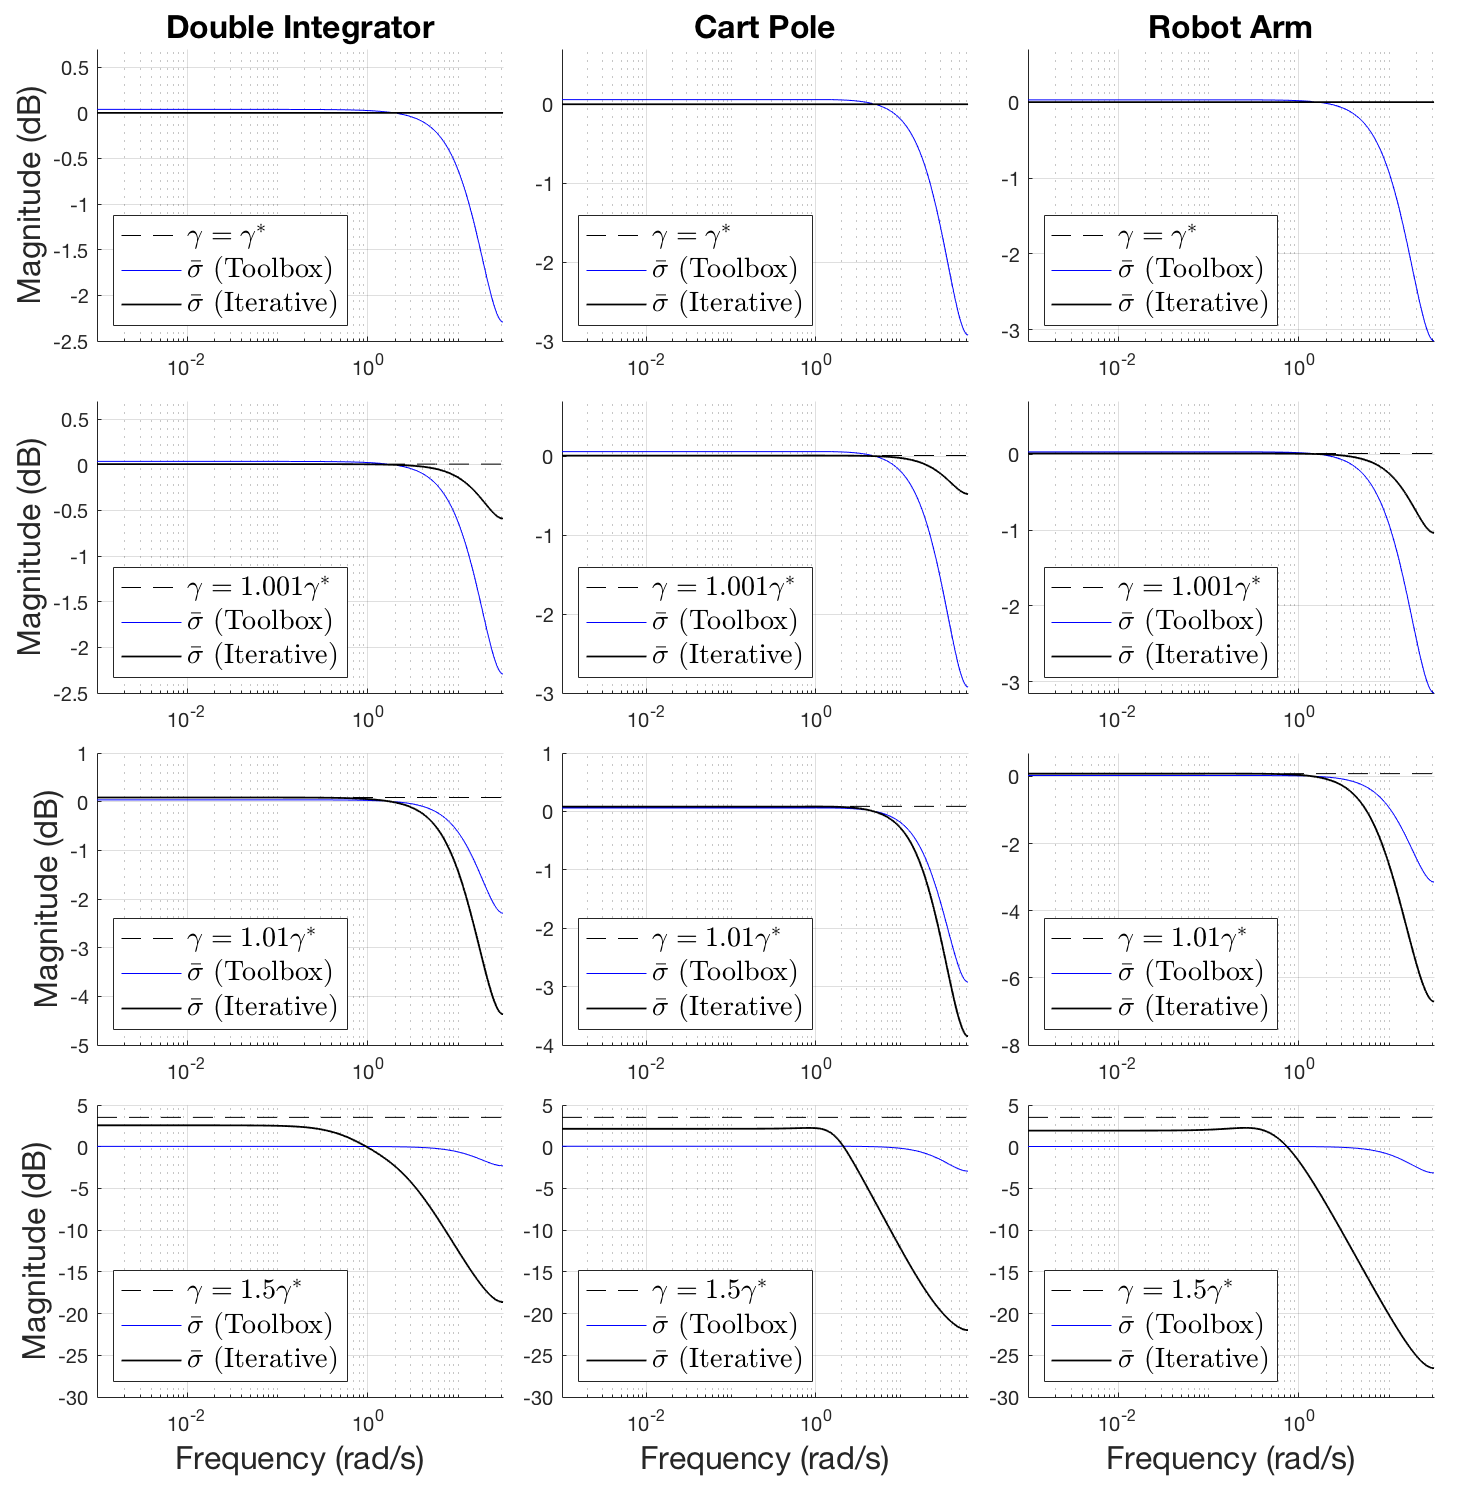
\includegraphics[width=\textwidth]{figures/waterbed_effect.png}
\caption{Loop shape for increasing $\gamma^{*}$, demonstrating the ``waterbed effect''.  Compared are an iterative DGARE solver (black) to \texttt{hinfsyn} from MATLAB's Robust Control Toolbox (blue).}
\label{fig:waterbed_effect}
\end{figure}

Figure \ref{fig:baseline_singular_values} shows the resulting nominal shape of the three case studies' frequency-dependent maximum singular values, relative to their respective minimax/optimal $\gamma^{*}$ (the 0 dB point) and the suboptimal design choice for $\gamma$ used for $\mathcal{H}_{\infty}$ control (the dotted black line).
\begin{figure}[H]
\centering
	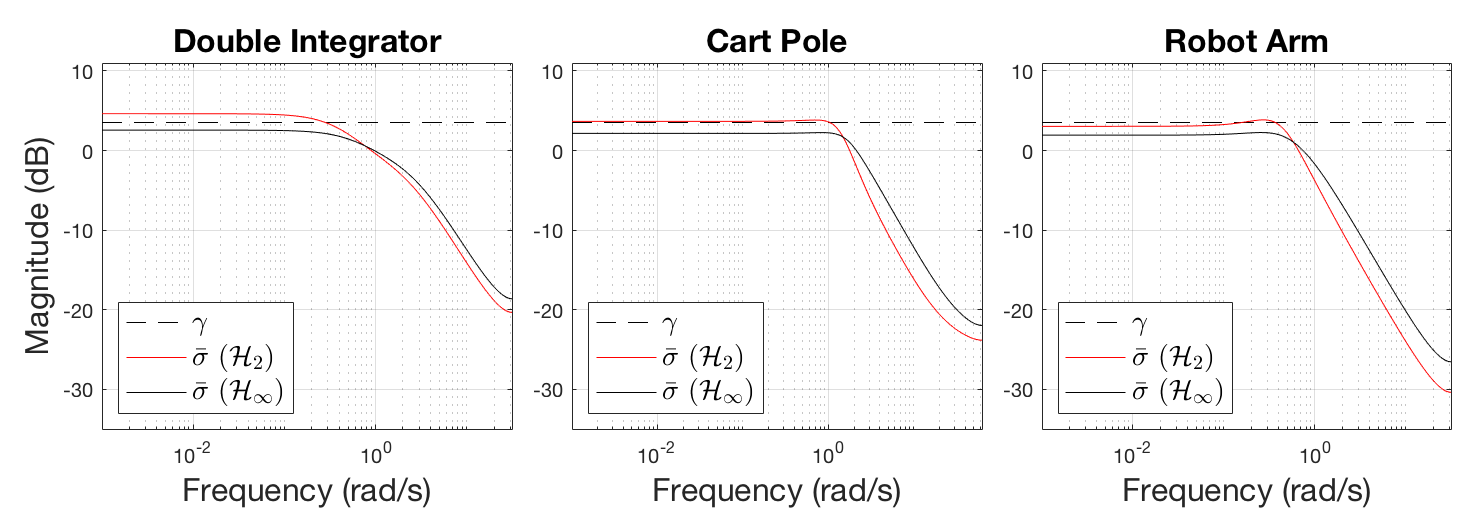
\includegraphics[width=\textwidth]{figures/baseline_singular_values.png}
\caption{Maximum singular values of the closed-loop generalized plants, for baseline controllers.}
\label{fig:baseline_singular_values}
\end{figure}

\subsection{Stability Margins}
One way to express robustness of a feedback system to gain or phase variations is the disk margin \cite{seiler2020introduction}, a scalar quantity which represents how much uncertainty the loop can tolerate before going unstable.  When used for control tuning, disk-based stability margins provide stronger guarantees of robustness than classical gain/phase margins since they take into account the interactions of all loops and frequencies.  In this work, disk-based margins for simultaneous input/output perturbations are computed using MATLAB's \texttt{diskmargin} routine from its Robust Control Toolbox, using the known open-loop plant and a given set of feedback gains.  The margins for the baseline systems are listed in Table \ref{table:baseline_disk_margins}.
\begin{table}[H]
\centering
\begin{tabular}{| l || c | c | c |} 
	\hline
	 & Double Integrator & Cart Pole & Robot Arm\\
	\hline\hline
	Baseline $\mathcal{H}_{2}$ & 1.183 & 0.542 & 0.739\\
	\hline
	Baseline $\mathcal{H}_{\infty}$ & 1.119 & 0.601 & 0.678\\
	\hline
\end{tabular}
\caption{Disk-based stability margins of baseline $\mathcal{H}_{2}$ and $\mathcal{H}_{\infty}$ feedback systems.}
\label{table:baseline_disk_margins}
\end{table}

\subsection{Transient Responses}
Figures \ref{fig:baseline_transient_double_integrator}, \ref{fig:baseline_transient_cart_pole} and \ref{fig:baseline_transient_robot_arm} show the transient responses of the three case study systems with the baseline $\mathcal{H}_{2}$ and $\mathcal{H}_{\infty}$ controllers.  The initial conditions of each system are selected to simulate the type of transient response in error dynamics which would immediately follow a closed-loop setpoint command, when the system is already in a stable state (zero velocity or rates).  For the double integrator, this simply means moving the system (e.g. the cart) to another position.  The cart pole moves the system to another position while also stabilizing the pole back to being upright.  The robot arm (without gravity) would similarly be moving from one angular position to another.

\begin{figure}[H]
\centering
	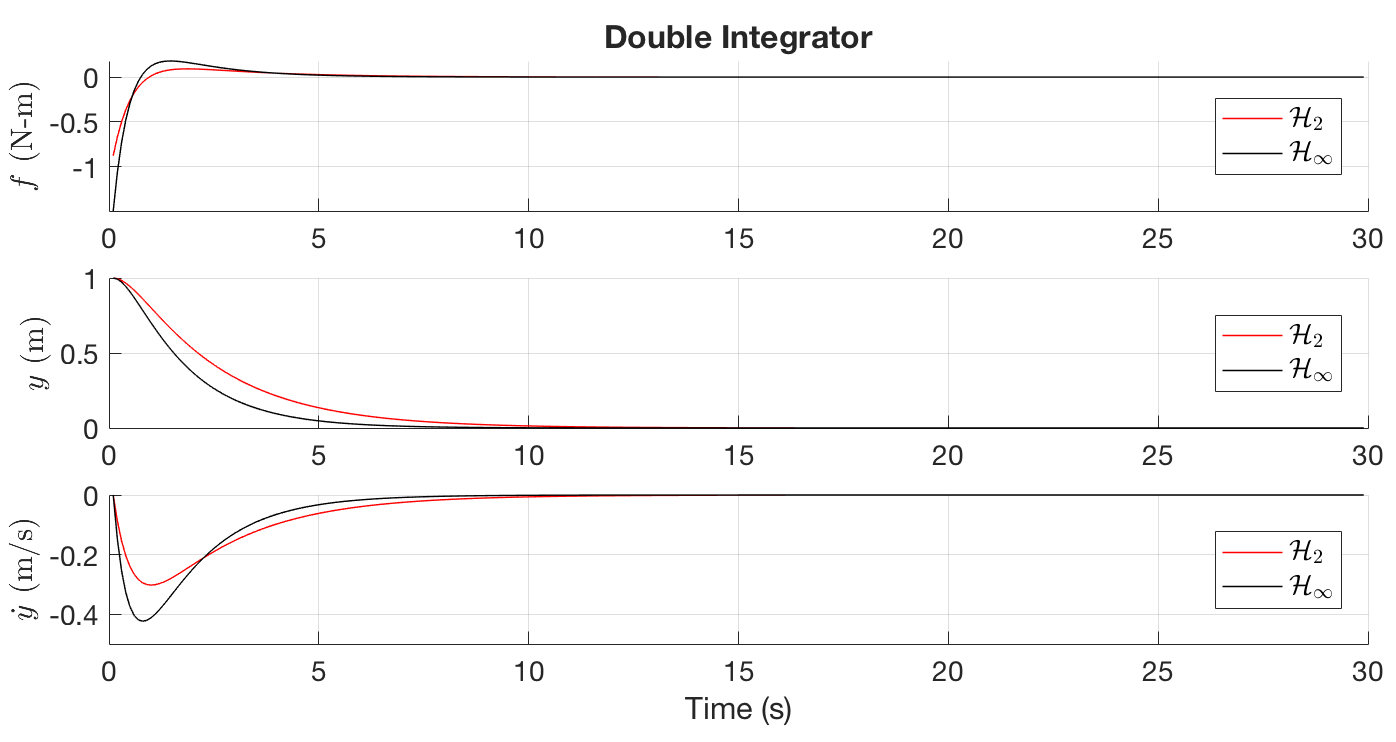
\includegraphics[width=\textwidth]{figures/baseline_transient_double_integrator.png}
\caption{Transient response of the closed-loop double integrator to non-zero initial conditions, for baseline controllers.}
\label{fig:baseline_transient_double_integrator}
\end{figure}

\begin{figure}[H]
\centering
	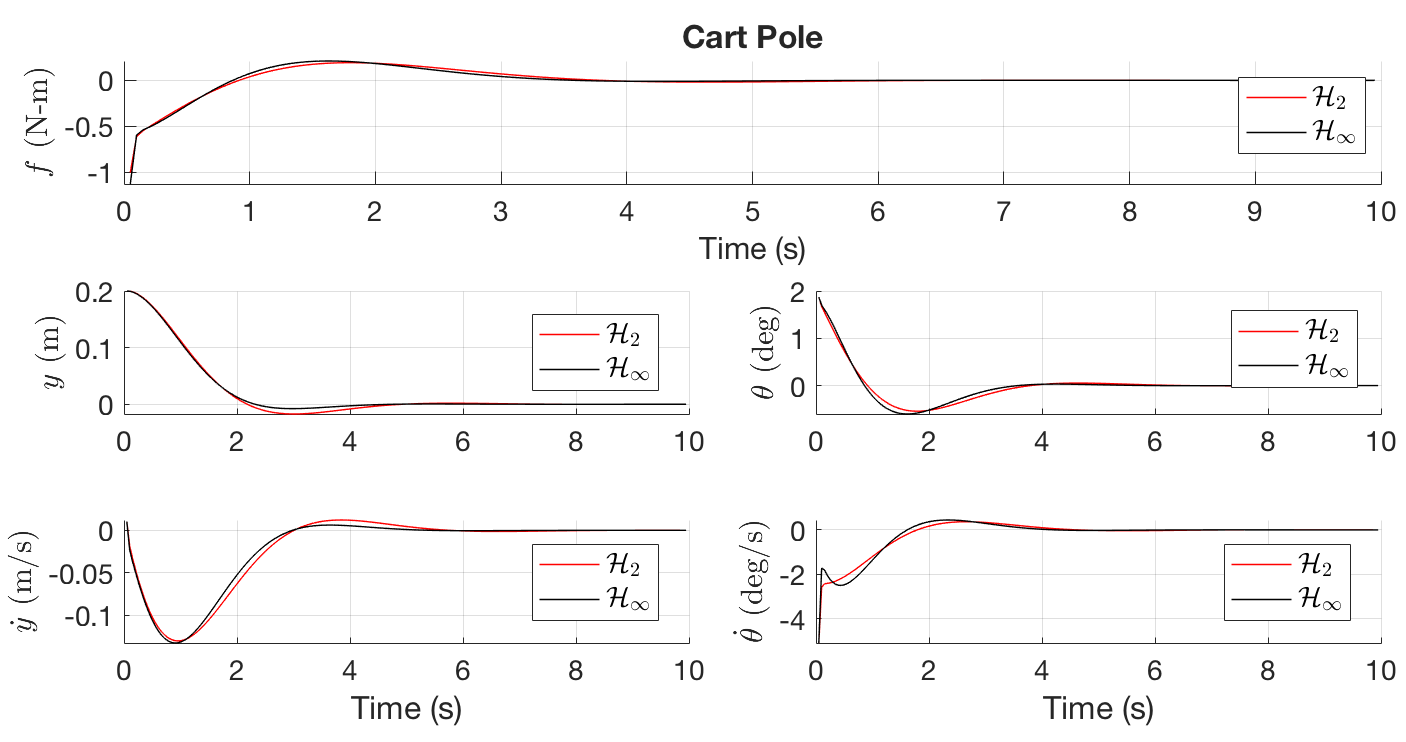
\includegraphics[width=\textwidth]{figures/baseline_transient_cart_pole.png}
\caption{Transient response of the closed-loop cart-pole to non-zero initial conditions, for baseline controllers.}
\label{fig:baseline_transient_cart_pole}
\end{figure}

\begin{figure}[H]
\centering
	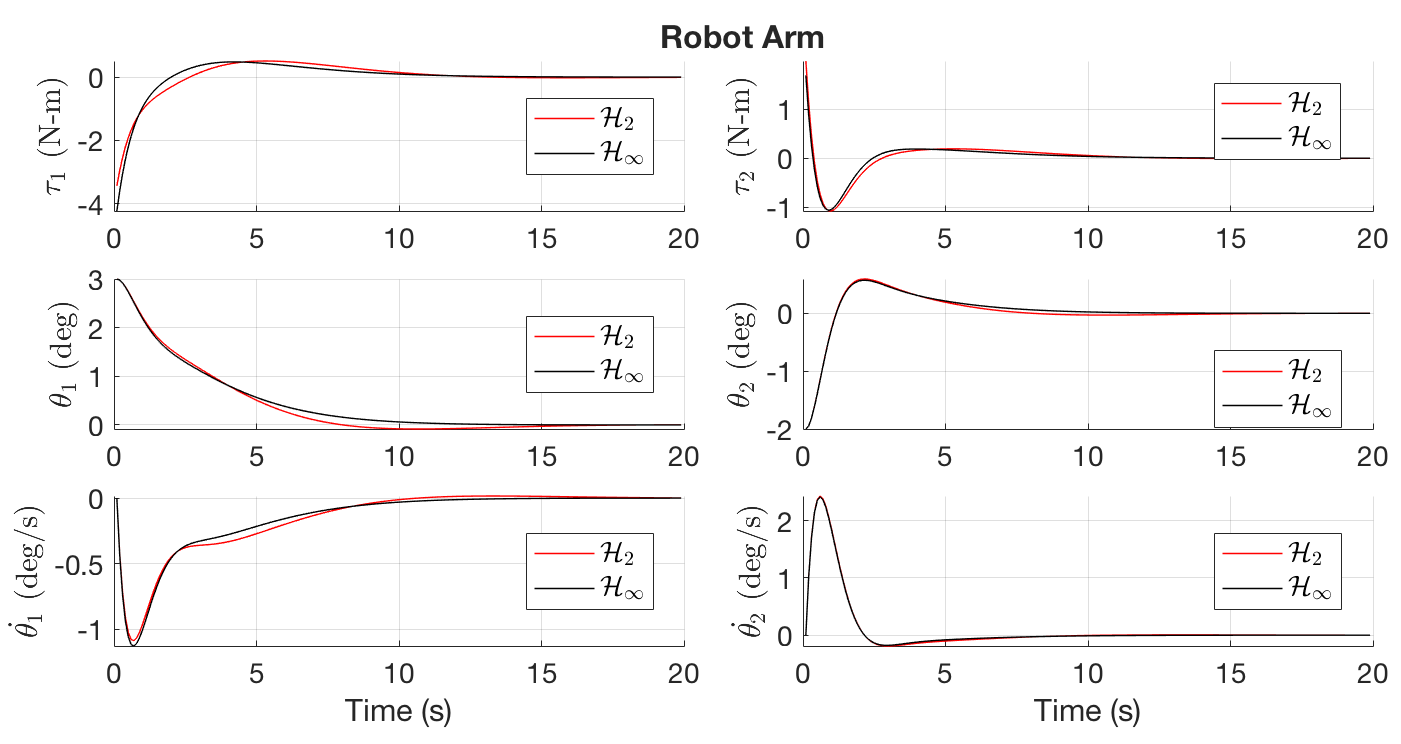
\includegraphics[width=\textwidth]{figures/baseline_transient_robot_arm.png}
\caption{Transient response of the closed-loop robot arm to non-zero initial conditions, for baseline controllers.}
\label{fig:baseline_transient_robot_arm}
\end{figure}

\subsection{Integrated Performance Metrics}
Figures \ref{fig:baseline_integrated_cost} shows the total integrated cost and control effort for each of the three case studies with $\mathcal{H}_{2}$ and $\mathcal{H}_{\infty}$ control.  The $\mathcal{H}_{\infty}$ control requires more control effort in all three cases, which leads to a rise in total LQ cost over the trajectory.  Note that in Figure \ref{fig:baseline_integrated_cost}, the integrated cost and control effort are both normalized to the infinite-horizon LQR cost.  This allows a standard comparison of performance relative to that which would be achieved with perfect model knowledge and zero disturbances.  The LQ cost plotted in the top row of Figure \ref{fig:baseline_integrated_cost} is given by Equation \ref{eq-optimal-cost-function}, and the control effort plotted in the bottom row of Figure \ref{fig:baseline_integrated_cost} is given by Equation \ref{eq:total-integrated-control-effort}.
\begin{equation}
\label{eq:total-integrated-control-effort}
\begin{aligned}
	J_{u} &= \lim_{N \to \infty} \sum_{k = 1}^{N} \big{(} \vb*{u}_{k}^{T} \vb*{u}_{k} \big{)}
\end{aligned}
\end{equation}

\begin{figure}[H]
\centering
	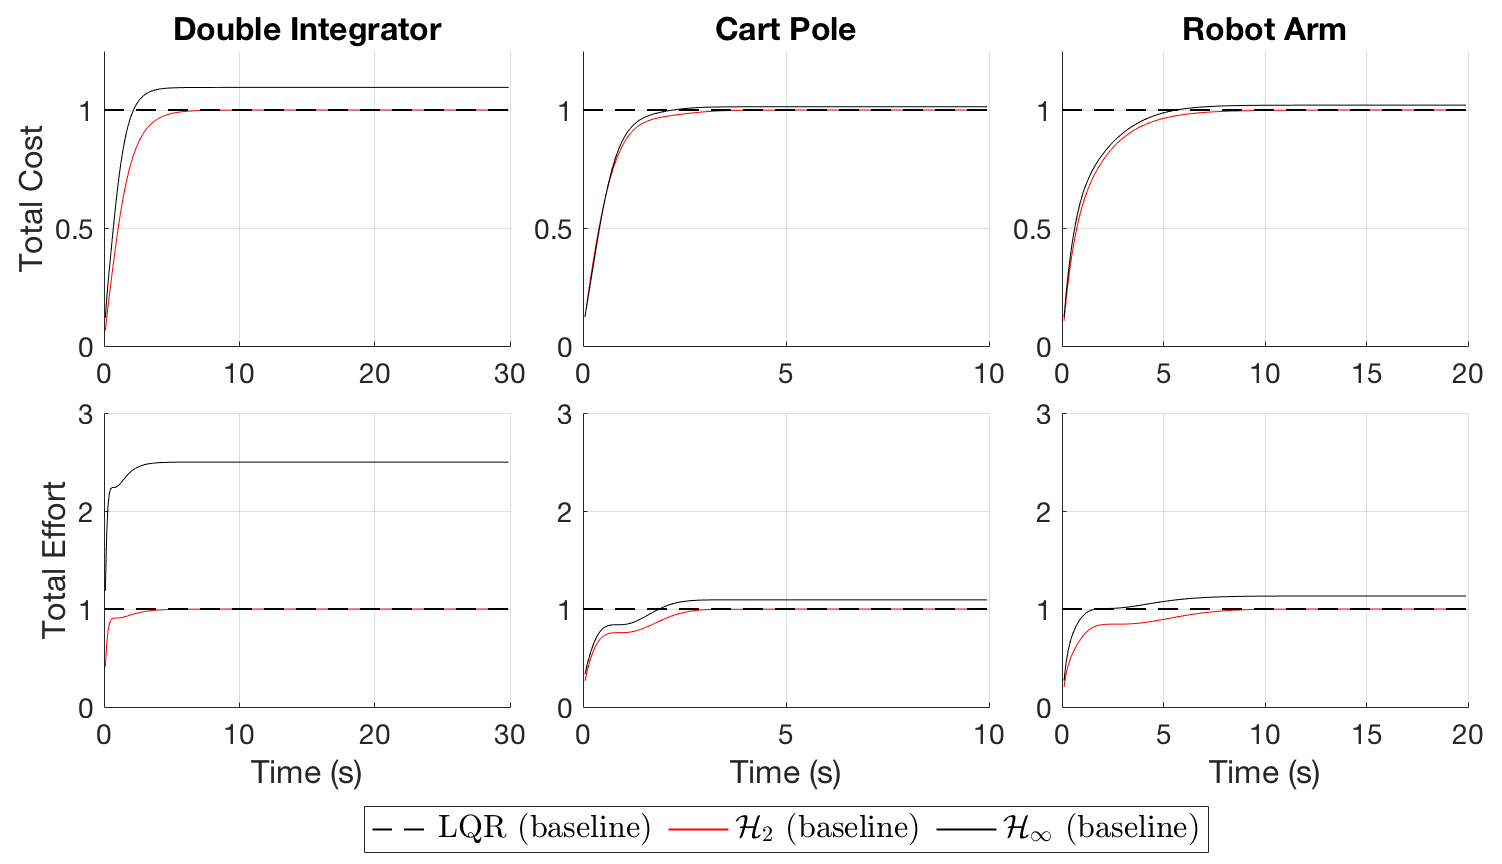
\includegraphics[width=\textwidth]{figures/baseline_integrated_cost.png}
\caption{Integrated cost and control effort of the closed-loop systems to non-zero initial conditions, for baseline controllers.}
\label{fig:baseline_integrated_cost}
\end{figure}

\section{Simulation Test Approach}
\label{sect:results:testapproach}
To test the effect of uncertainty and noise on both indirect and direct data-driven control, a repeated-trial test is used to evaluate each case study.  There are two test scenarios: learning to control a system with parameter uncertainty, and learning to control a system with measurement noise.  It is expected that while measurement noise should have no effect on the ability to compute baseline control designs, it will certainly affect the efficacy of learning controllers from data, and may affect the performance of both types when simulated.

For a separate sweep of each of the two scale factors (from 0\% to 60\%), 100 different test runs are evaluated for different data-driven control methods, to compare to baseline model-based control methods.  Each run gathers a finite trajectory of training data from the fully-nonlinear plant, and using this data several data-driven controllers are computed.  If they are stable, their robustness metrics are compared to the baseline case.

Indirect approaches use the DMDc algorithm given by Equation \eqref{eq:dmdc_solution} to estimate a linear discrete-time plant model from the training data, followed by model-based $\mathcal{H}_{2}$ and (suboptimal) $\mathcal{H}_{\infty}$ control.  Direct approaches implement the LMIs given by Equations \eqref{eq:h2_lmi_dd} and \eqref{eq:h2s_lmi_dd} which solve model-free optimizations for $\mathcal{H}_{2}$ optimal and $\mathcal{H}_{2}$ suboptimal control, respectively.  These leverage the MATLAB-based CVX parser \cite{grant2008graph, grant2008cvx} with its default SDPT3 \cite{toh1999sdpt3, tutuncu2001sdpt3} and SeDuMi \cite{sturm1999using} SDP solvers.

For a given scale factor, several metrics are computed and averaged across the 100 test runs.  The first metric is the fraction of stabilizing data-driven controllers; those which do not keep the system poles within the unit circle are marked as unstable.  For those which are stable, the closed-loop disk margin (see Appendix \ref{appendix:sensitivity}) and $\mathcal{H}_{\infty}$ norms are compared to characterize the robustness of the controllers synthesized from data.

Additionally, the full feedback system is then simulated with fixed duration and initial conditions to obtain integrated control effort and LQ cost, to characterize performance.  However, those whose integrated metrics or $\mathcal{H}_{\infty}$ norms are disproportionately large (at least 10 times above the average) are marked unstable and their metrics are discarded.

\underline{\textbf{Note:}} Because unstable controllers cannot be included in the calculation of robustness metrics, average values (nominally out of 100 samples) become skewed when the fraction of stable controllers dwindles

\subsection{Training Policies}
Table \ref{table:training_policies} summarizes the control policies used to gather an $N$-sample state-input trajectory of training data.  In general, these were a linear combination of a stabilizing state feedback law with gains $\vb*{K}_{0}$, a time-varying input $\vb*{u}_{expl}(t_{k})$ to promote exploration, i.e.,
\begin{equation}
\begin{aligned}
	\vb*{u} &= \vb*{K}_{0}\vb*{x}_{k} + \vb*{u}_{expl}(t_{k})
\end{aligned}
\end{equation}
and the values of $\vb*{K}_{0}$ were selected heuristically.   These merely keep the closed-loop system stable, and are generally not optimized for robustness or performance.
\begin{table}[H]
\centering
\begin{tabular}{|c || c | c | c|} 
	\hline
	 & $\vb*{K}_{0}$ & $\vb*{u}_{expl}(t_{k})$ & $N$\\
	\hline\hline
	Double Integrator & $\begin{bmatrix} -1.91 & -1.01\end{bmatrix}$ & $0.1\exp(-0.8t_{k})\sin(4t_{k}) + \mathcal{N}(0, 0.5)$ & 80\\ 
	\hline
	Cart Pole & $\begin{bmatrix}-2 & 3 & -3 & 7\end{bmatrix}$ & $10.1\exp(-0.8t_{k})\sin(t_{k})$ & 100\\
	\hline
	Robot Arm & $\begin{bmatrix}-60 & -3 & -200 & -60\\ -3 & -60 & -60 & -68\end{bmatrix}$ & $\begin{bmatrix}
		10\exp(-0.8t_{k})\sin(t_{k}) + \mathcal{N}(0, 0.05)\\ 10\exp(-0.8t_{k})\sin(t_{k}) + \mathcal{N}(0, 0.05) \end{bmatrix}$ & 150\\
	\hline
\end{tabular}
\caption{Control policies used to gather training data.}
\label{table:training_policies}
\end{table}

\newpage
\subsection{Parameter Uncertainty Test Harness}
Here, a single inertial parameter from each case study system was selected to be uncertain.  For the double integrator, this was the mass ($m_{c}$), for the cart-pole it was the pole length ($l$) and for the robot arm this was the length of link 1 ($l_{1}$).  These parameters were subjected to a zero-mean Gaussian additive disturbance with a variance that is some fraction of their nominal value.  Pseudocode for this test is given by Algorithm \ref{alg:scaled_uncertainty_test}, which is applied to each of the three case studies.

\begin{algorithm}
\caption{Test harness for simulating single parameter uncertainty.}
\label{alg:scaled_uncertainty_test}
\begin{algorithmic}
	\State Calculate baseline model-based control gains ($\mathcal{H}_{2}$, $\mathcal{H}_{\infty}$):
	\State \hspace{10pt} $\vb*{K}_{2}^{b} \gets $ baseline $\mathcal{H}_{2}$ synthesis
	\State \hspace{10pt} $\vb*{K}_{\infty}^{b} \gets $ baseline $\mathcal{H}_{\infty}$ synthesis
	\For{scale factor in $ \begin{bmatrix} 0, & 0.1, & 0.2, & 0.3, & 0.4, & 0.5, & 0.6 \end{bmatrix}$}
		\State $n \gets 1$
		\While{$n < 100$}
			\State Perturb system parameter according to scale factor.
			\State Compute off-nominal linearized plant model.
			\State Simulate full off-nominal system to obtain training data.
			\State Use training data to compute data-driven control gains ($\mathcal{H}_{2}$, $\mathcal{H}_{\infty}$):
			\State \hspace{10pt} $\vb*{K}_{2}^{i} \gets $ indirect $\mathcal{H}_{2}$ synthesis
			\State \hspace{10pt} $\vb*{K}_{2}^{d} \gets $ direct $\mathcal{H}_{2}$ synthesis
			\State \hspace{10pt} $\vb*{K}_{\infty}^{i} \gets $ indirect $\mathcal{H}_{\infty}$ synthesis
			\For{$\vb*{K}$ in $\begin{bmatrix} \vb*{K}_{2}^{b}, & \vb*{K}_{\infty}^{b}, & \vb*{K}_{2}^{i}, & \vb*{K}_{2}^{d}, & \vb*{K}_{\infty}^{i} \end{bmatrix}$}
				\State Use off-nominal plant to compute closed-loop stability of $(\vb*{A} - \vb*{B}\vb*{K})$.
				\If{stable}
					\State Compute disk margin using sensitivity function $(\vb*{S} - \vb*{T})/2$.
					\State Compute $\mathcal{H}_{\infty}$ norm using generalized plant $\vb*{T}_{K}$.
					\State Simulate full system with $\vb*{u}_{k} = -\vb*{K}\vb*{x}_{k}$, from initial conditions $(\vb*{x}_{0},\vb*{u}_{0})$.
					\State Compute total integrated control effort and total integrated LQ cost.
				\Else
					\State Test failed; discard and set all metrics to NaN.
				\EndIf
			\EndFor
		\State $n \gets n + 1$
		\EndWhile
	\EndFor
\end{algorithmic}
\end{algorithm}

\subsection{Measurement Noise Test Harness}
Here, a rough estimate of nominal variance was assumed for each system.  This was then scaled in a similar fashion as the parameter uncertainty.  Nominal variance was taken as 0.1 m$^{2}$ for position, 0.05 m$^{2}$s$^{-2}$ for linear velocity, 0.1deg$^{2}$ for angles and 0.01deg$^{2}$s$^{-2}$ for angular rates.  Maximum values were taken to be twice the nominal values, and the scale factor was applied to the maximum values.  Pseudocode for this test is given by Algorithm \ref{alg:scaled_noise_test}, which is applied to each of the three case studies.

\begin{algorithm}
\caption{Test harness for simulating measurement noise.}
\label{alg:scaled_noise_test}
\begin{algorithmic}
	\State Calculate baseline model-based control gains ($\mathcal{H}_{2}$, $\mathcal{H}_{\infty}$):
	\State \hspace{10pt} $\vb*{K}_{2}^{b} \gets $ baseline $\mathcal{H}_{2}$ synthesis
	\State \hspace{10pt} $\vb*{K}_{\infty}^{b} \gets $ baseline $\mathcal{H}_{\infty}$ synthesis
	\For{scale factor in $ \begin{bmatrix} 0, & 0.1, & 0.2, & 0.3, & 0.4, & 0.5, & 0.6 \end{bmatrix}$}
		\State Adjust variance of measurement noise according to scale factor.
		\State $n \gets 1$
		\While{$n < 100$}
			\State Simulate full noisy system to obtain training data.
			\State Use training data to compute data-driven control gains ($\mathcal{H}_{2}$, $\mathcal{H}_{\infty}$):
			\State \hspace{10pt} $\vb*{K}_{2}^{i} \gets $ indirect $\mathcal{H}_{2}$ synthesis
			\State \hspace{10pt} $\vb*{K}_{2}^{d} \gets $ direct $\mathcal{H}_{2}$ synthesis
			\State \hspace{10pt} $\vb*{K}_{\infty}^{i} \gets $ indirect $\mathcal{H}_{\infty}$ synthesis
			\For{$\vb*{K}$ in $\begin{bmatrix} \vb*{K}_{2}^{b}, & \vb*{K}_{\infty}^{b}, & \vb*{K}_{2}^{i}, & \vb*{K}_{2}^{d}, & \vb*{K}_{\infty}^{i} \end{bmatrix}$}
				\State Use nominal plant to compute closed-loop stability of $(\vb*{A} - \vb*{B}\vb*{K})$.
				\If{stable}
					\State Compute disk margin using sensitivity function $(\vb*{S} - \vb*{T})/2$.
					\State Compute $\mathcal{H}_{\infty}$ norm using generalized plant $\vb*{T}_{K}$.
					\State Simulate full system with $\vb*{u}_{k} = -\vb*{K}\vb*{x}_{k}$, from initial conditions $(\vb*{x}_{0},\vb*{u}_{0})$.
					\State Compute total integrated control effort and total integrated LQ cost.
				\Else
					\State Test failed; discard and set all metrics to NaN.
				\EndIf
			\EndFor
		\State $n \gets n + 1$
		\EndWhile
	\EndFor
\end{algorithmic}
\end{algorithm}

\chapter{Results and Analysis}
\label{chap:results}
This chapter describes the design and results of simulations that evaluate the robustness of certain data-driven techniques.  This includes singular values (of the generalized plant), disk-based stability margins, transient responses, and integrated cost/effort metrics.  Results from the tests described in Section \ref{sect:results:testapproach} are given in the following sections.  Section \ref{sect:results:data-driven-optimal} plots the results of data-driven $\mathcal{H}_{2}$ and $\mathcal{H}_{\infty}$ optimal control.  Similar plots are provided in Section \ref{sect:results:data-driven-suboptimal}, except the data-driven $\mathcal{H}_{2}$ design uses the ``suboptimal'' performance objective described in Section \ref{sect:dataDrivenH2Suboptimal}.  Section \ref{sect:results:discussion} discusses the overall trends in the results with a focus on the effect of uncertainty, noise, and choice of performance objective.

\newpage
\section{Test Results: Data-Driven $\mathcal{H}_{2}$ and $\mathcal{H}_{\infty}$}
\label{sect:results:data-driven-optimal}
These included data-driven $\mathcal{H}_{2}$ (direct and indirect) and $\mathcal{H}_{\infty}$ (indirect).
\subsection{Parameter Uncertainty}
\subsubsection{Singular Values}
\begin{figure}[H]
\centering
	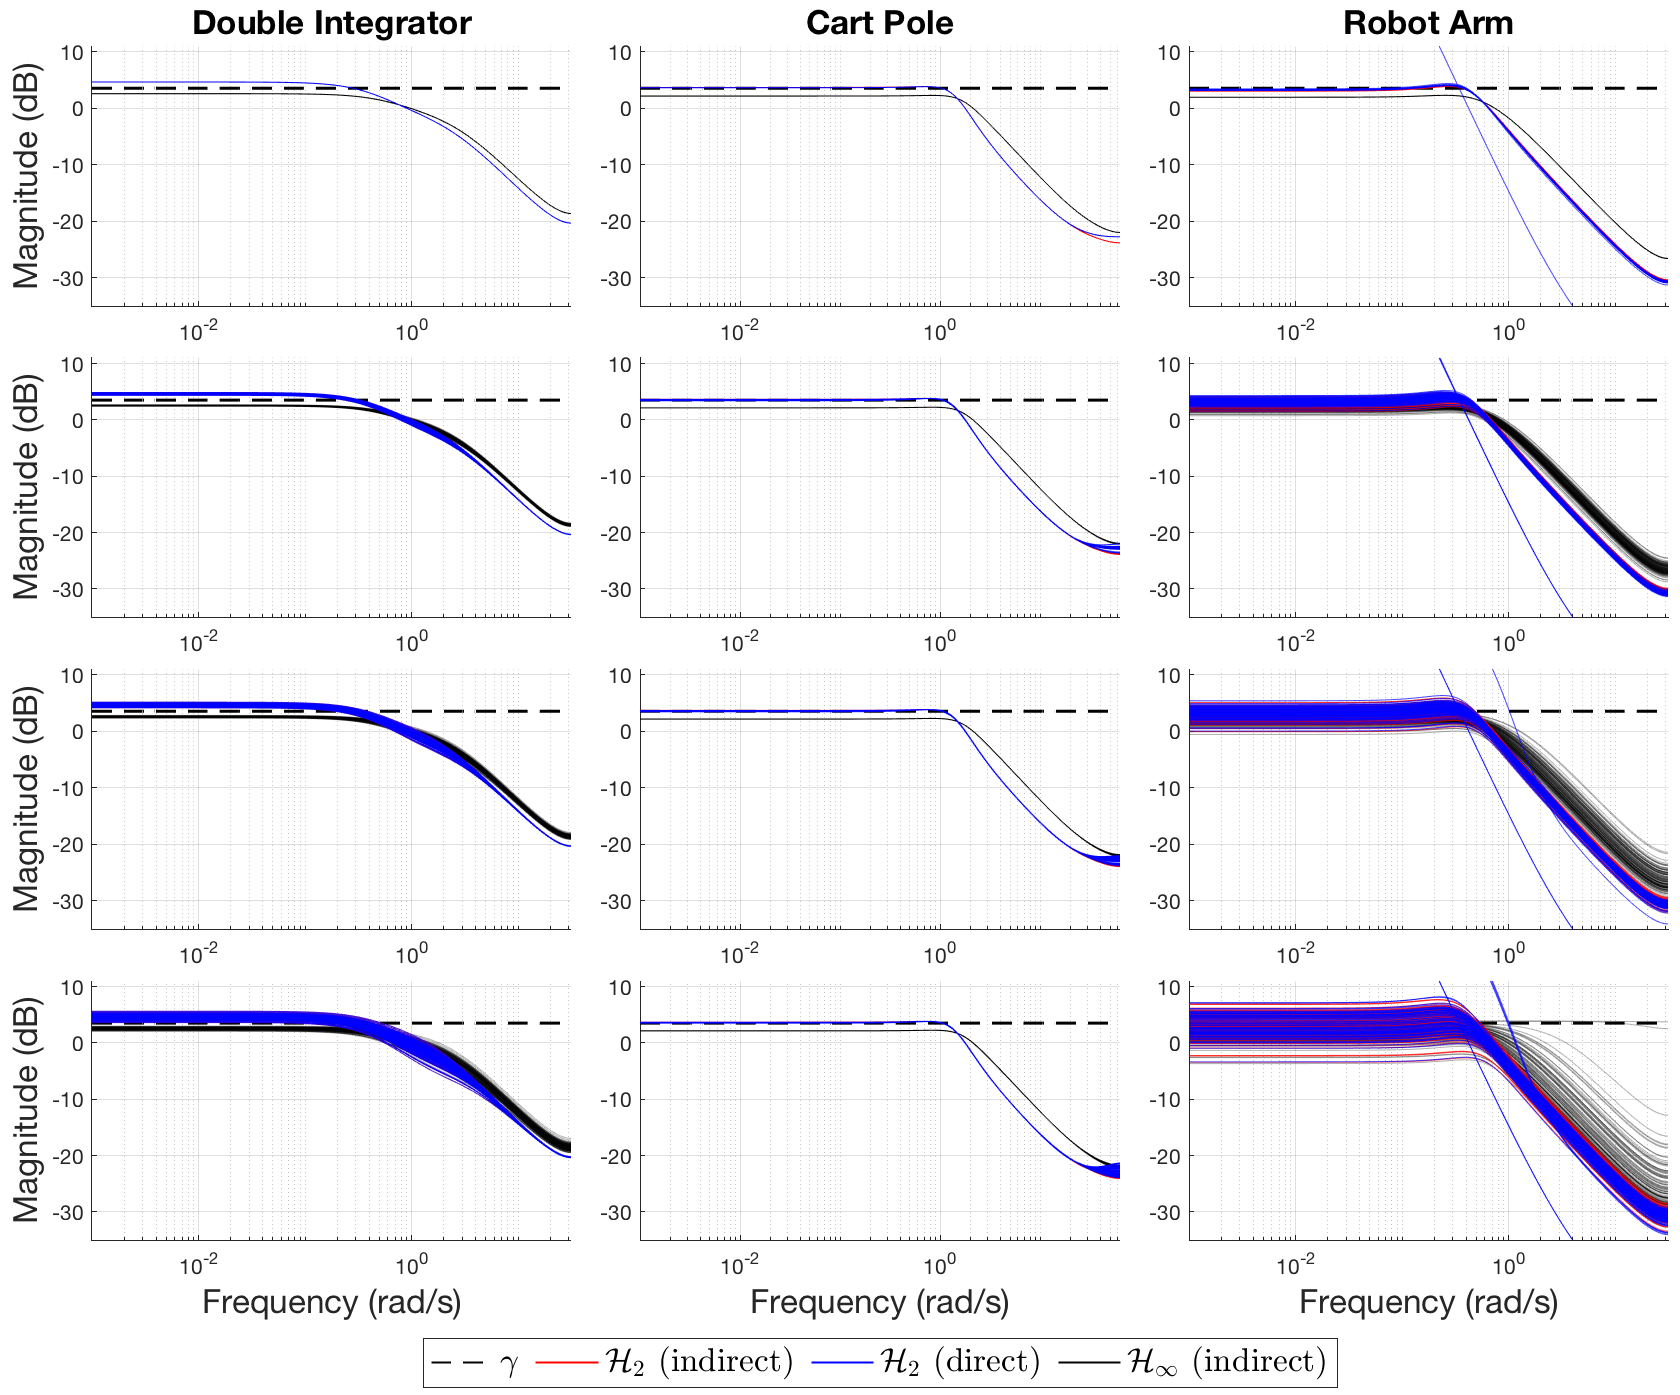
\includegraphics[width=\textwidth]{figures/uncertainty_singular_values3.png}
\caption{Maximum singular values of the closed-loop generalized plant, for controllers learned from systems with single-parameter uncertainty.  The rows correspond to respective scale factors of 0\%, 5\%, 10\%, and 20\%.  For each scale factor, the plots from 100 test runs are overlaid.}
\label{fig:uncertainty_singular_values3}
\end{figure}

\newpage
\subsubsection{Integrated Control Effort}
\begin{figure}[H]
\centering
	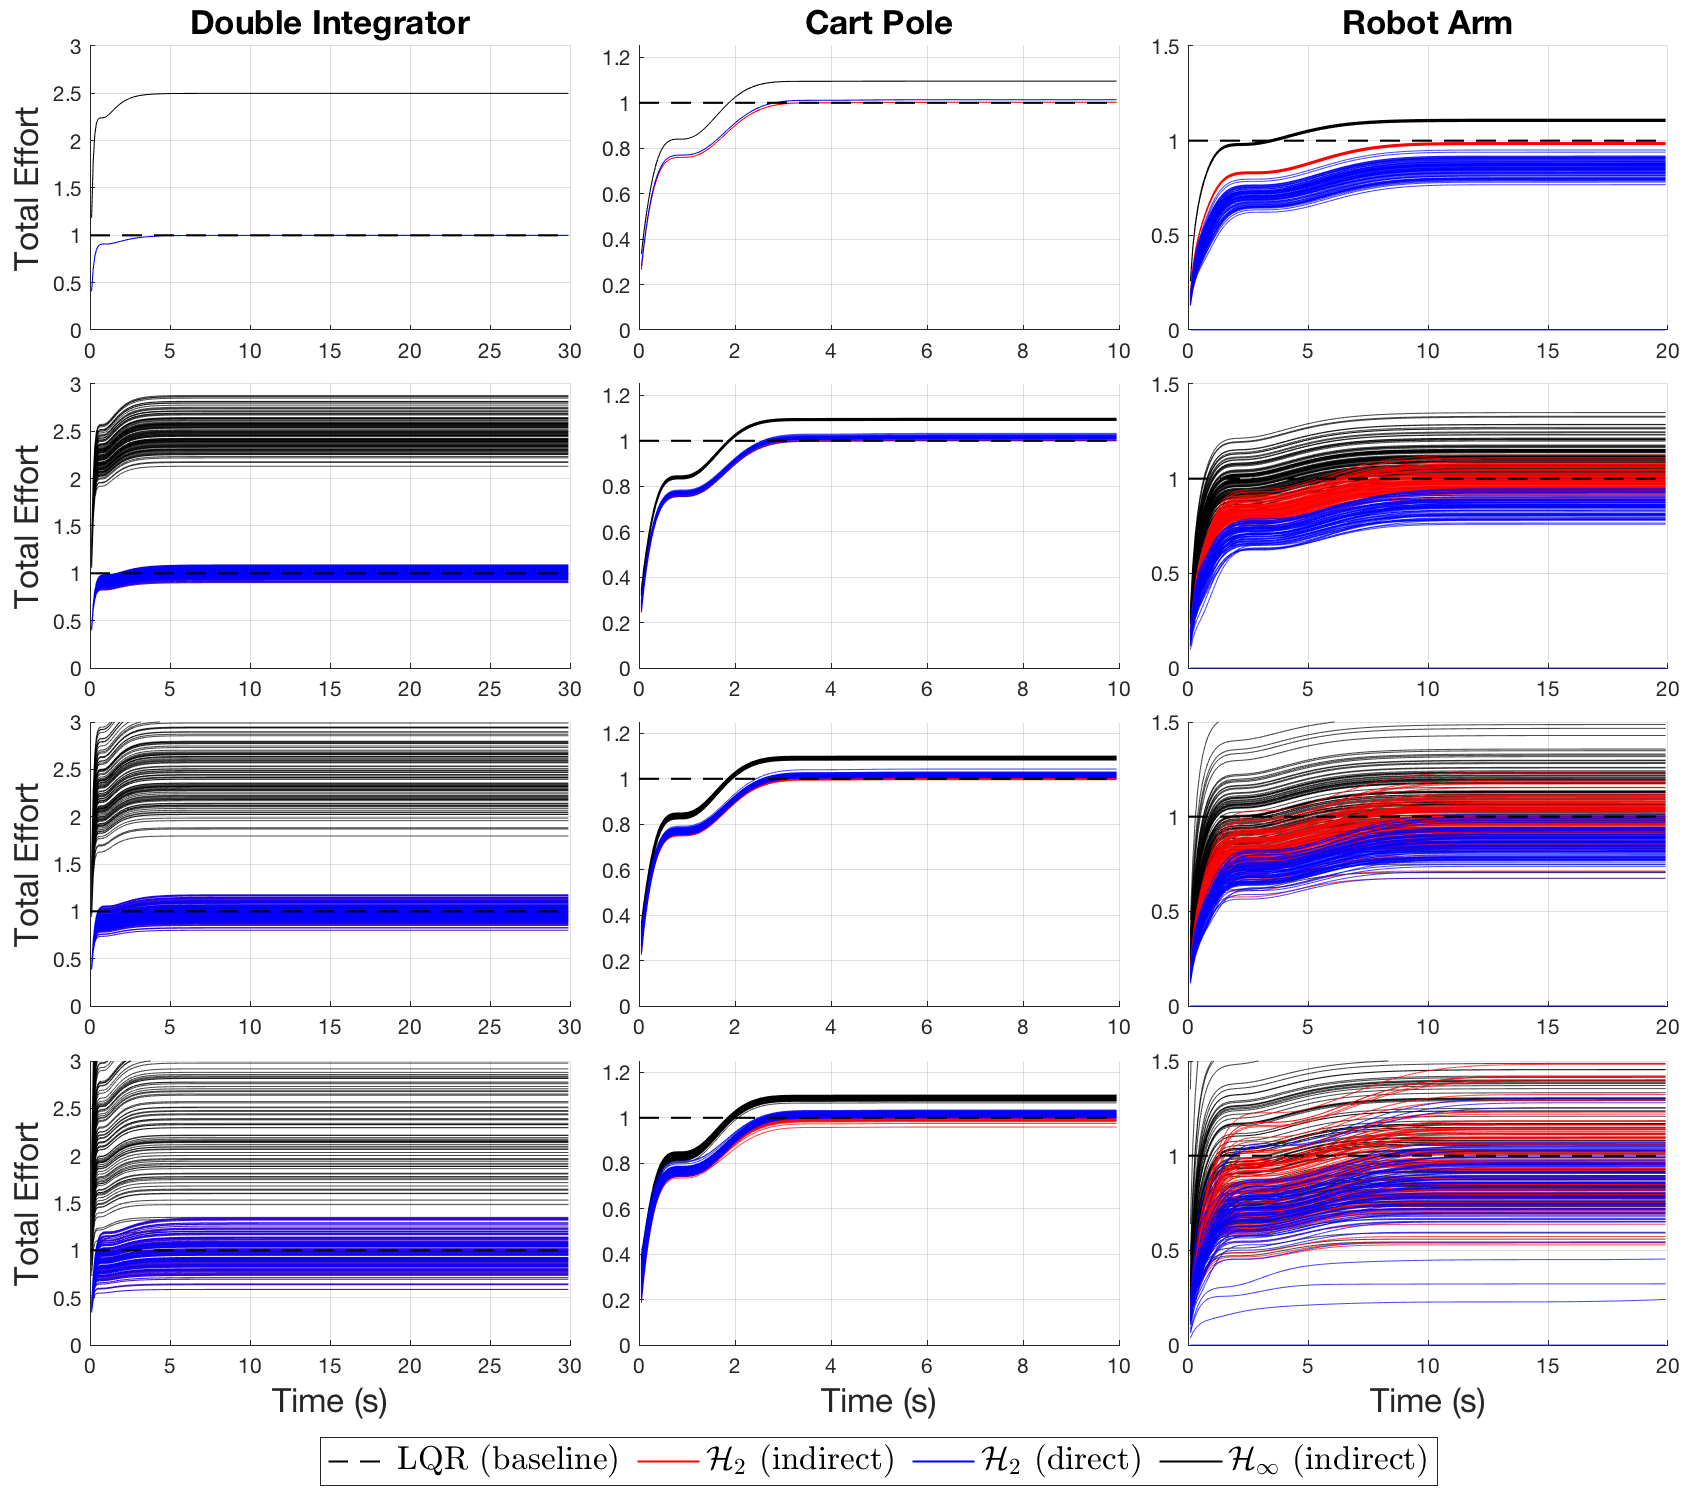
\includegraphics[width=\textwidth]{figures/uncertainty_integrated_effort3.png}
\caption{Integrated control effort of the closed-loop generalized plant, for controllers learned from systems with single-parameter uncertainty.  The rows correspond to respective scale factors of 0\%, 5\%, 10\%, and 20\%.  For each scale factor, the plots from 100 test runs are overlaid.}
\label{fig:uncertainty_integrated_effort3}
\end{figure}

\newpage
\subsubsection{Integrated LQ Cost}
\begin{figure}[H]
\centering
	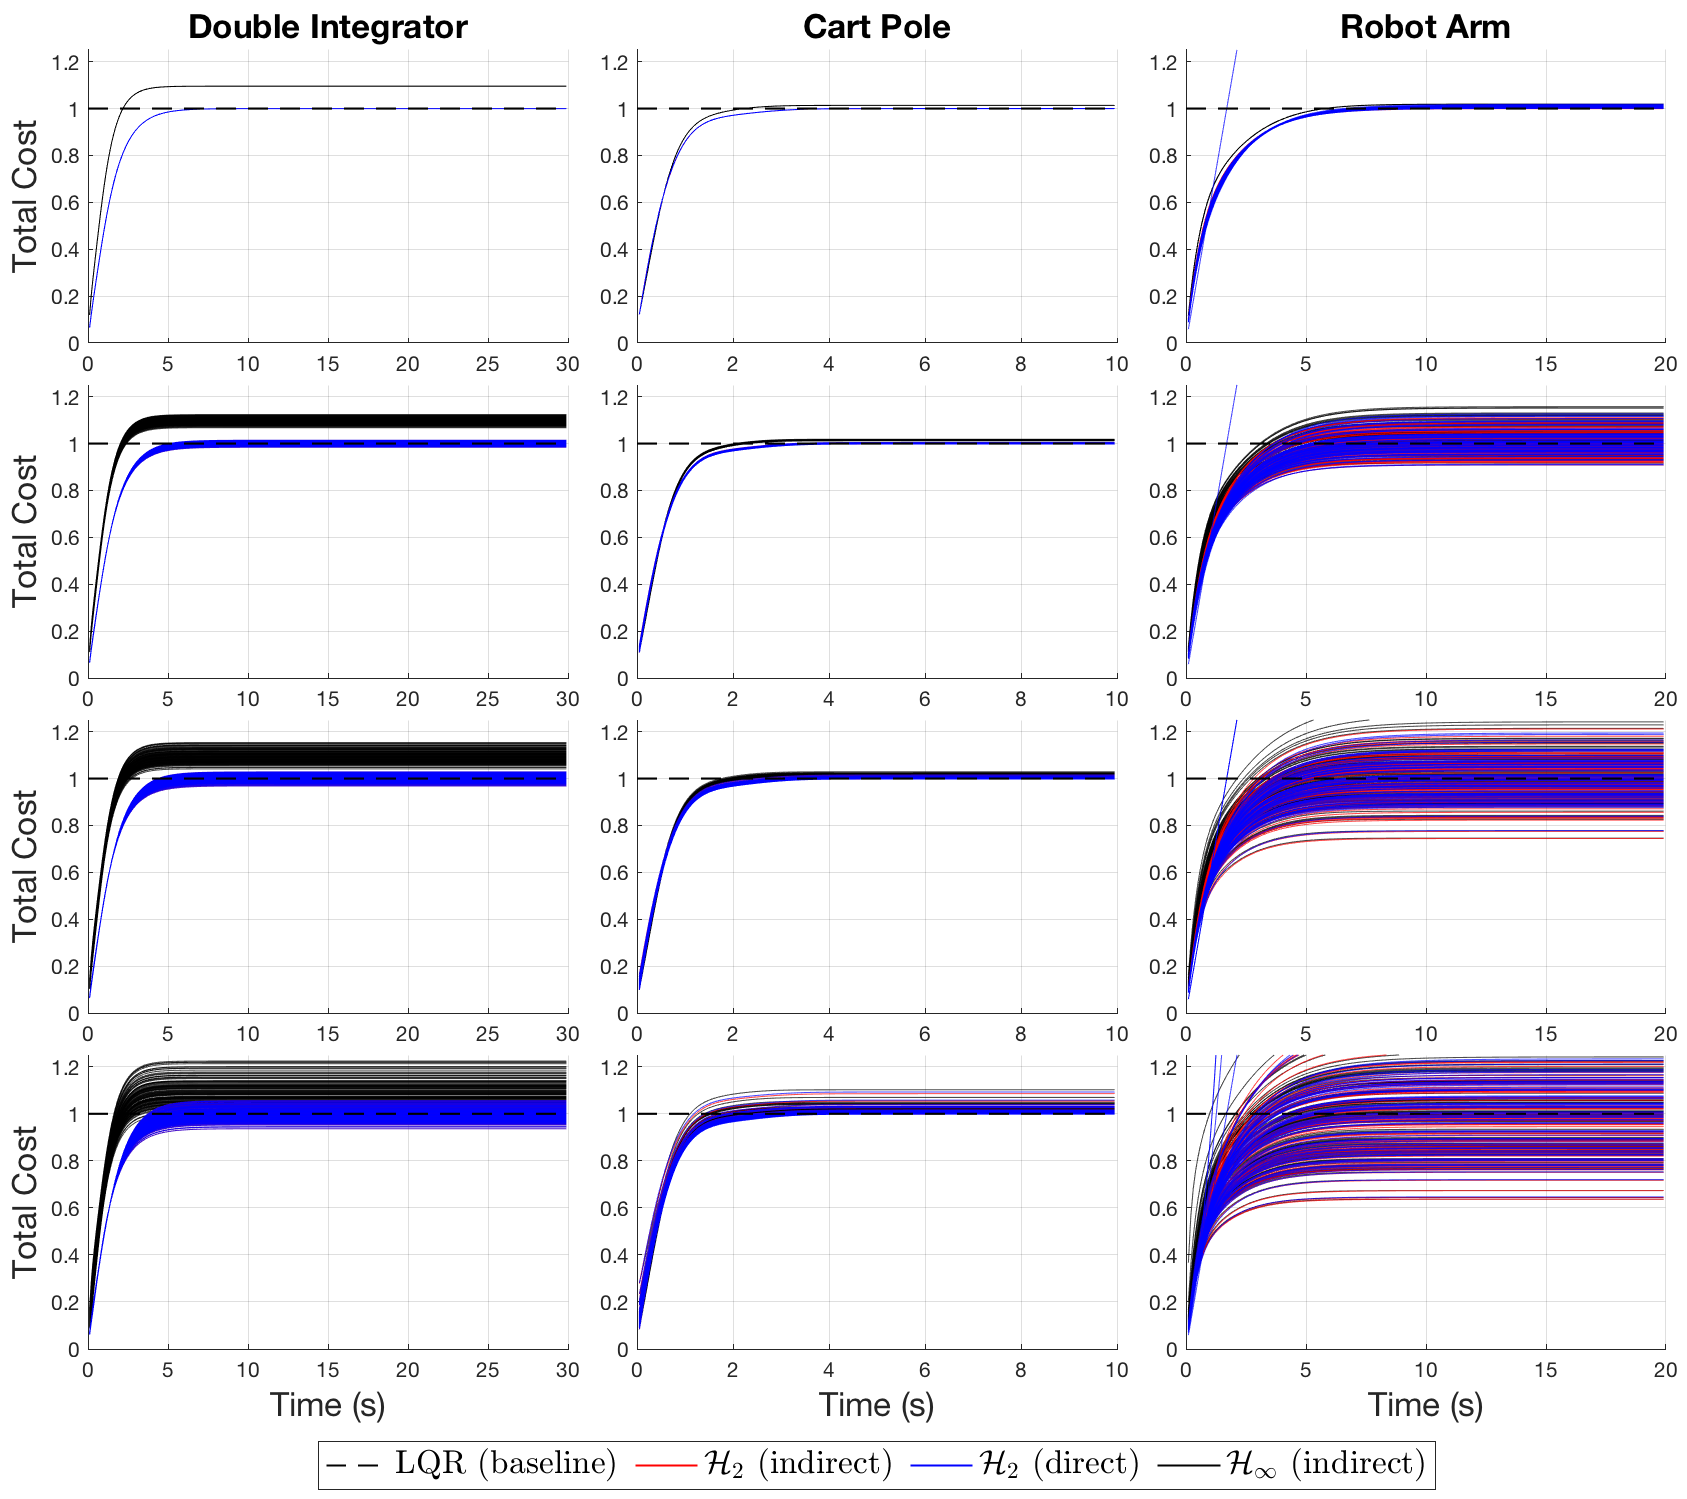
\includegraphics[width=\textwidth]{figures/uncertainty_integrated_cost3.png}
\caption{Integrated LQ cost of the closed-loop generalized plant, for controllers learned from systems with single-parameter uncertainty.  The rows correspond to respective scale factors of 0\%, 5\%, 10\%, and 20\%.  For each scale factor, the plots from 100 test runs are overlaid.}
\label{fig:uncertainty_integrated_cost3}
\end{figure}

\newpage
\subsubsection{Overall Trends}
\underline{\textbf{Note}}: Averaged metrics shown in Figure \ref{fig:overall_trends_uncertainty_opt_bar} are only defined for stable controllers, and may be skewed when the ``percent stable'' metric is significantly below 100\%.
\begin{figure}[H]
\centering
	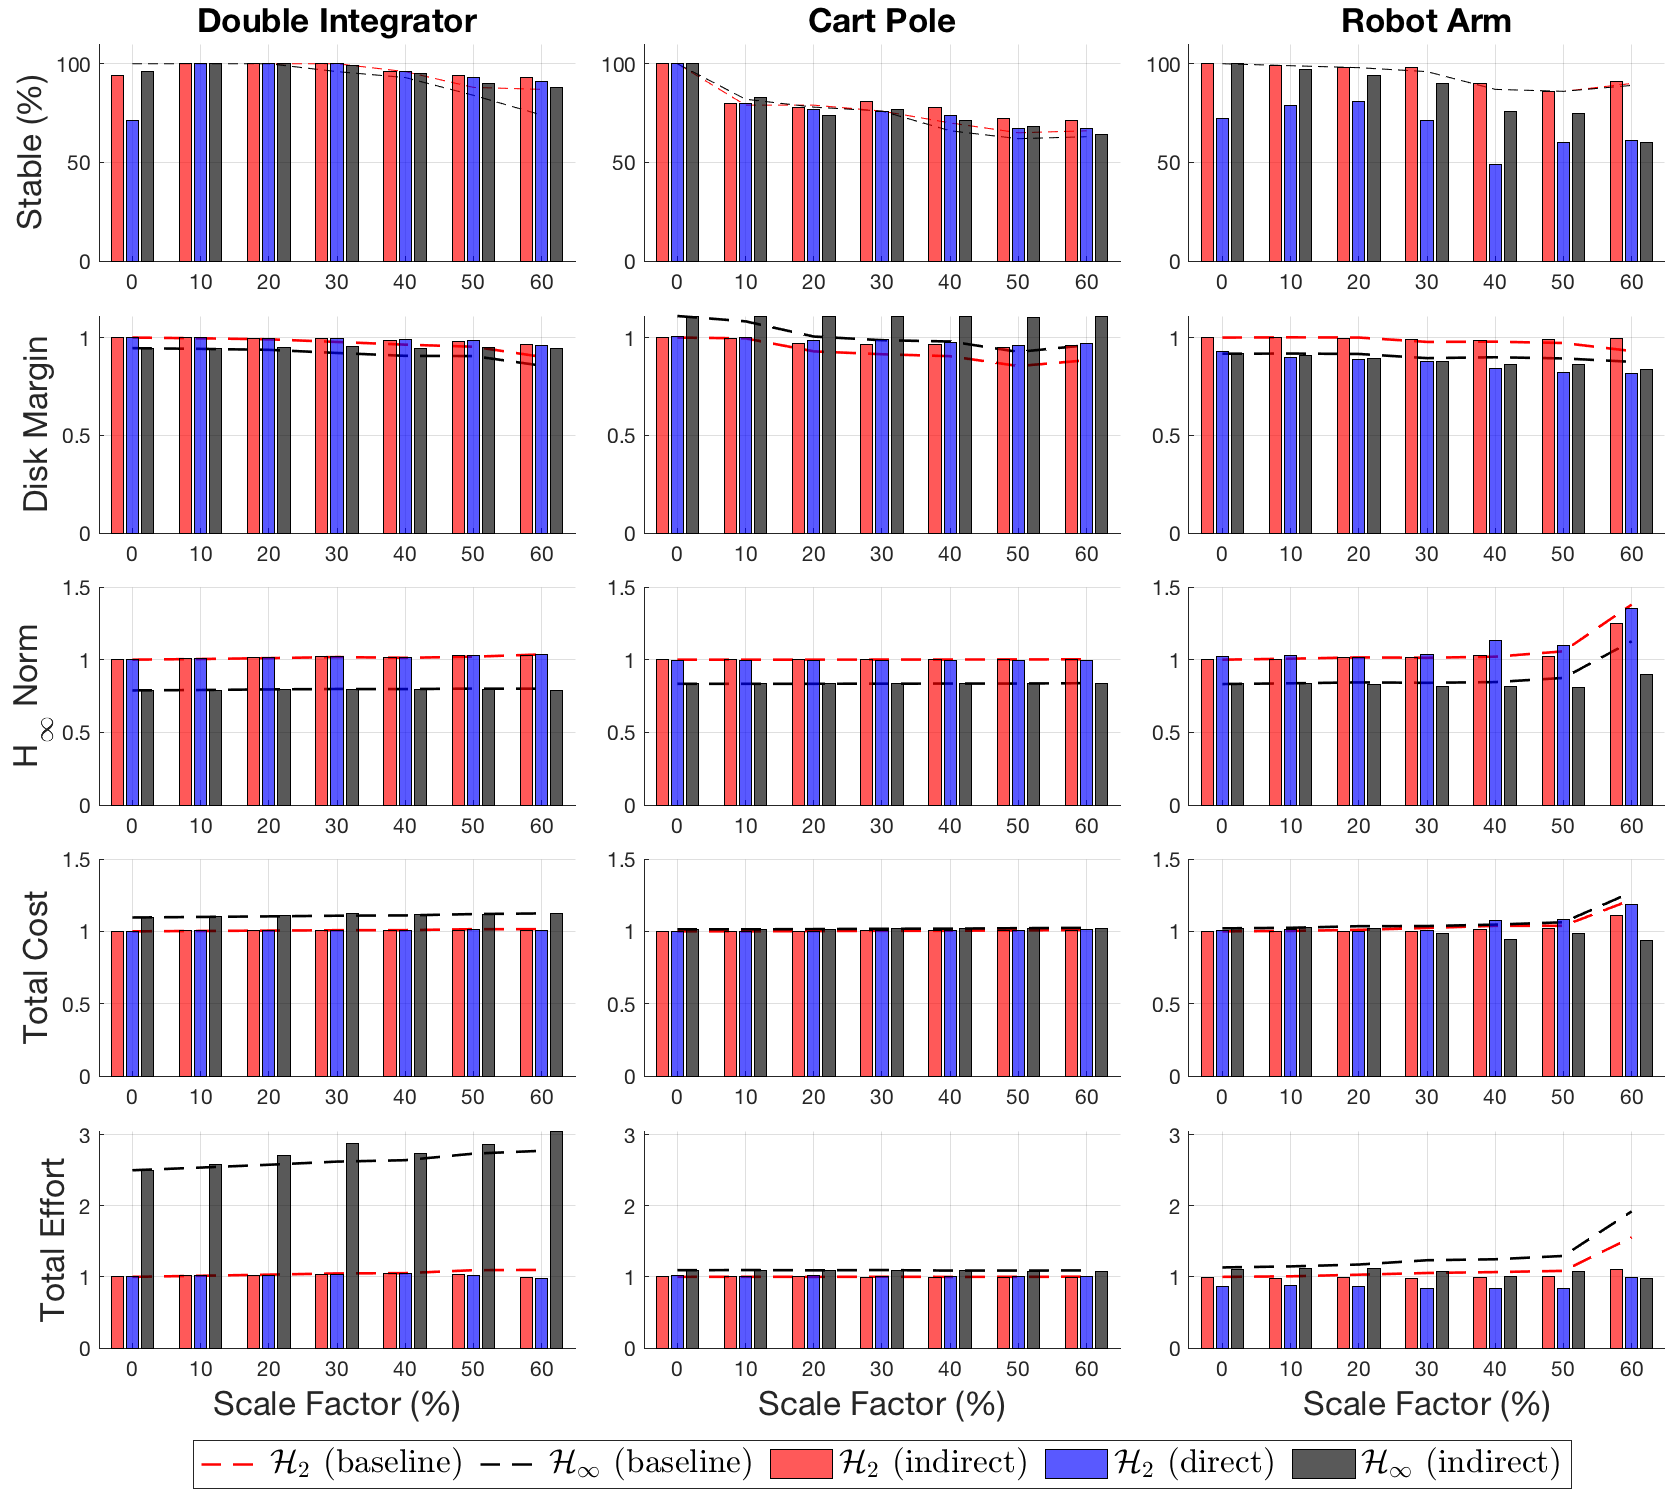
\includegraphics[width=\textwidth]{figures/overall_trends_uncertainty_opt_bar.png}
\caption{Overall trends for scaled uncertainty tests, comparing data-driven to baseline control approaches.  Apart from the percentage of stable controllers, all other metrics are normalized to what would be obtained by a nominal LQR/$\mathcal{H}_{2}$ feedback controller.  For each scale factor, the metrics shown are averaged across the stable test runs.}
\label{fig:overall_trends_uncertainty_opt_bar}
\end{figure}

\newpage
\subsection{Measurement Noise}
\subsubsection{Singular Values}
\begin{figure}[H]
\centering
	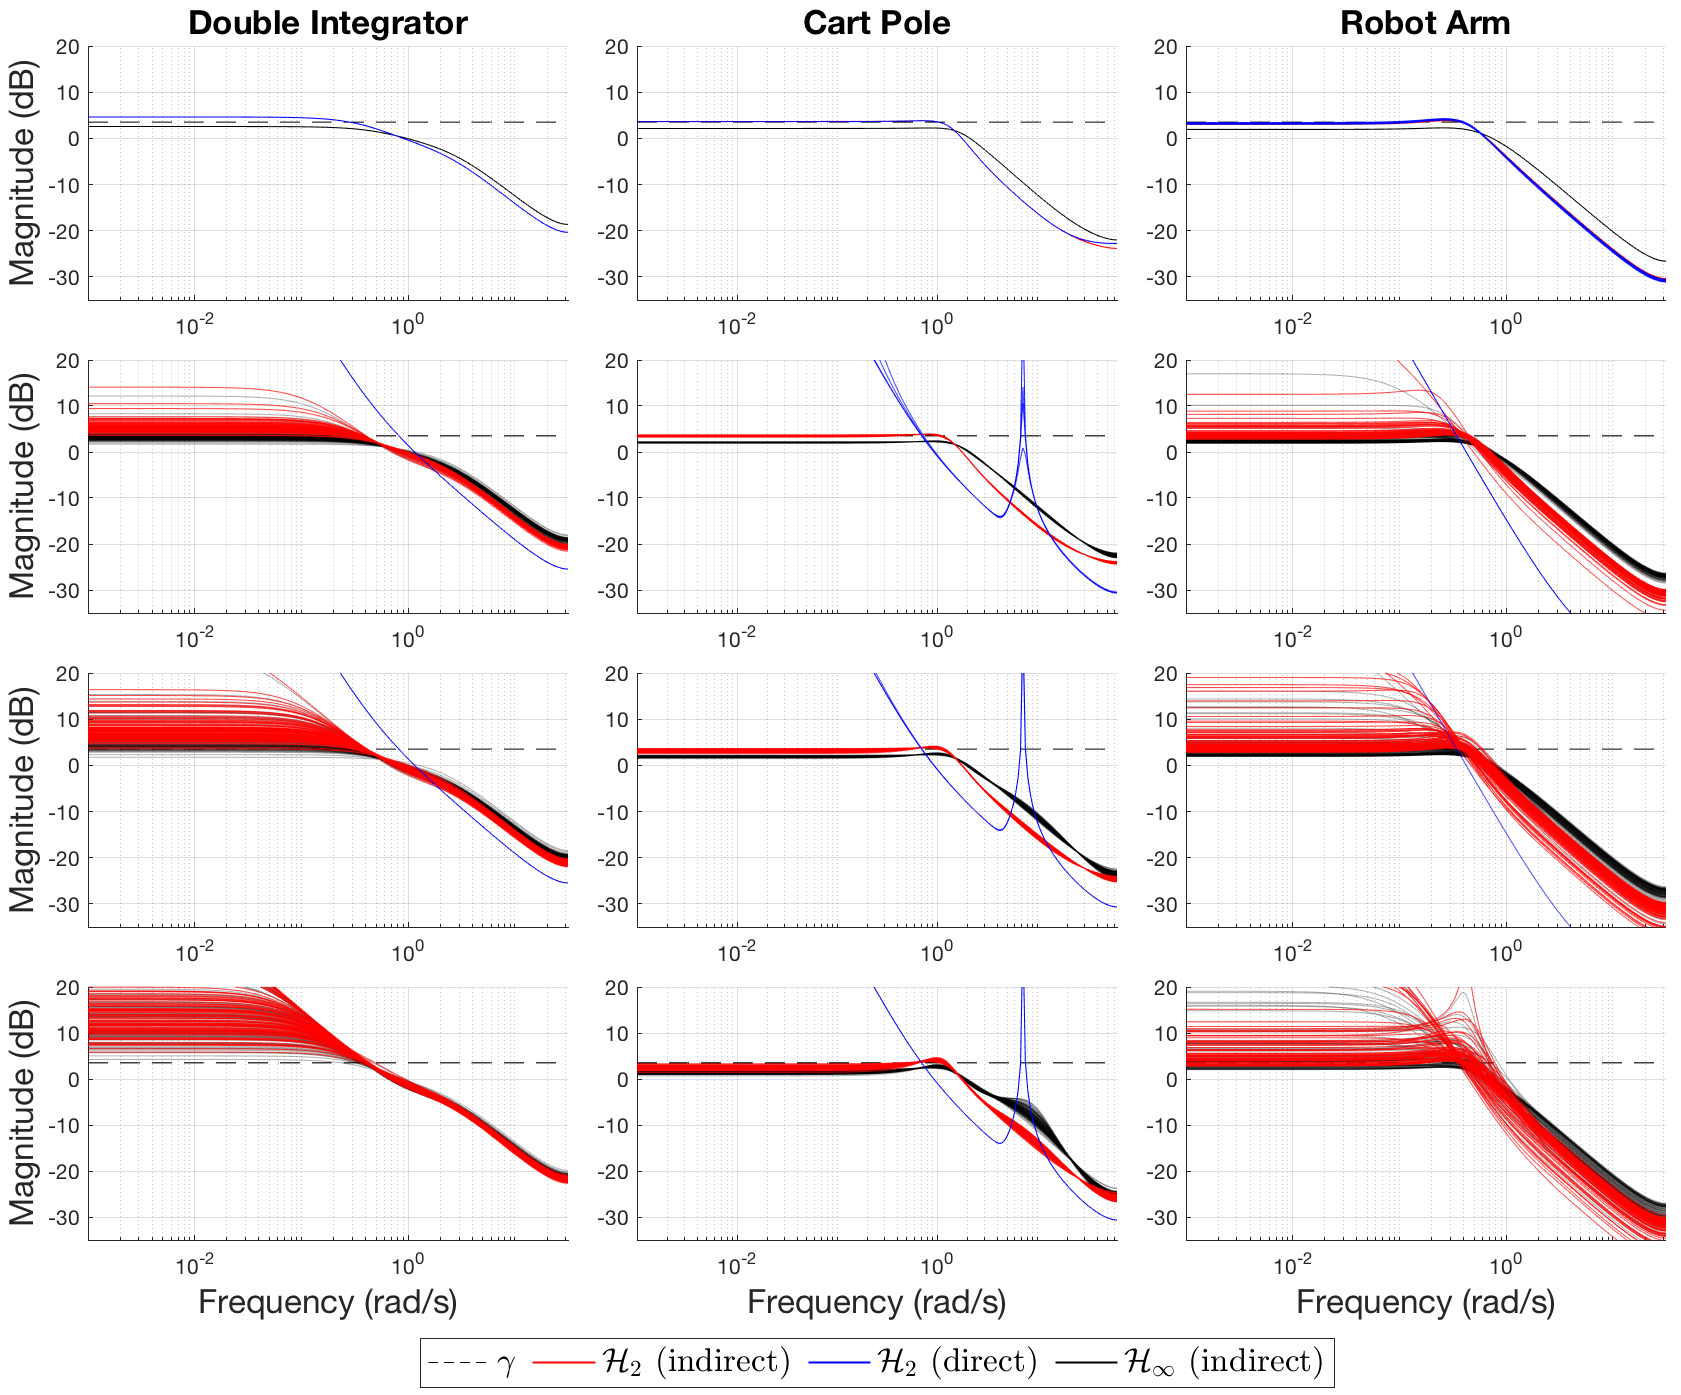
\includegraphics[width=\textwidth]{figures/noise_singular_values3.png}
\caption{Maximum singular values of the closed-loop generalized plant, for controllers learned from systems with measurement noise.  The rows correspond to respective scale factors of 0\%, 5\%, 10\%, and 20\%.  For each scale factor, the plots from 100 test runs are overlaid.}
\label{fig:noise_singular_values3}
\end{figure}

\newpage
\subsubsection{Integrated Control Effort}
\begin{figure}[H]
\centering
	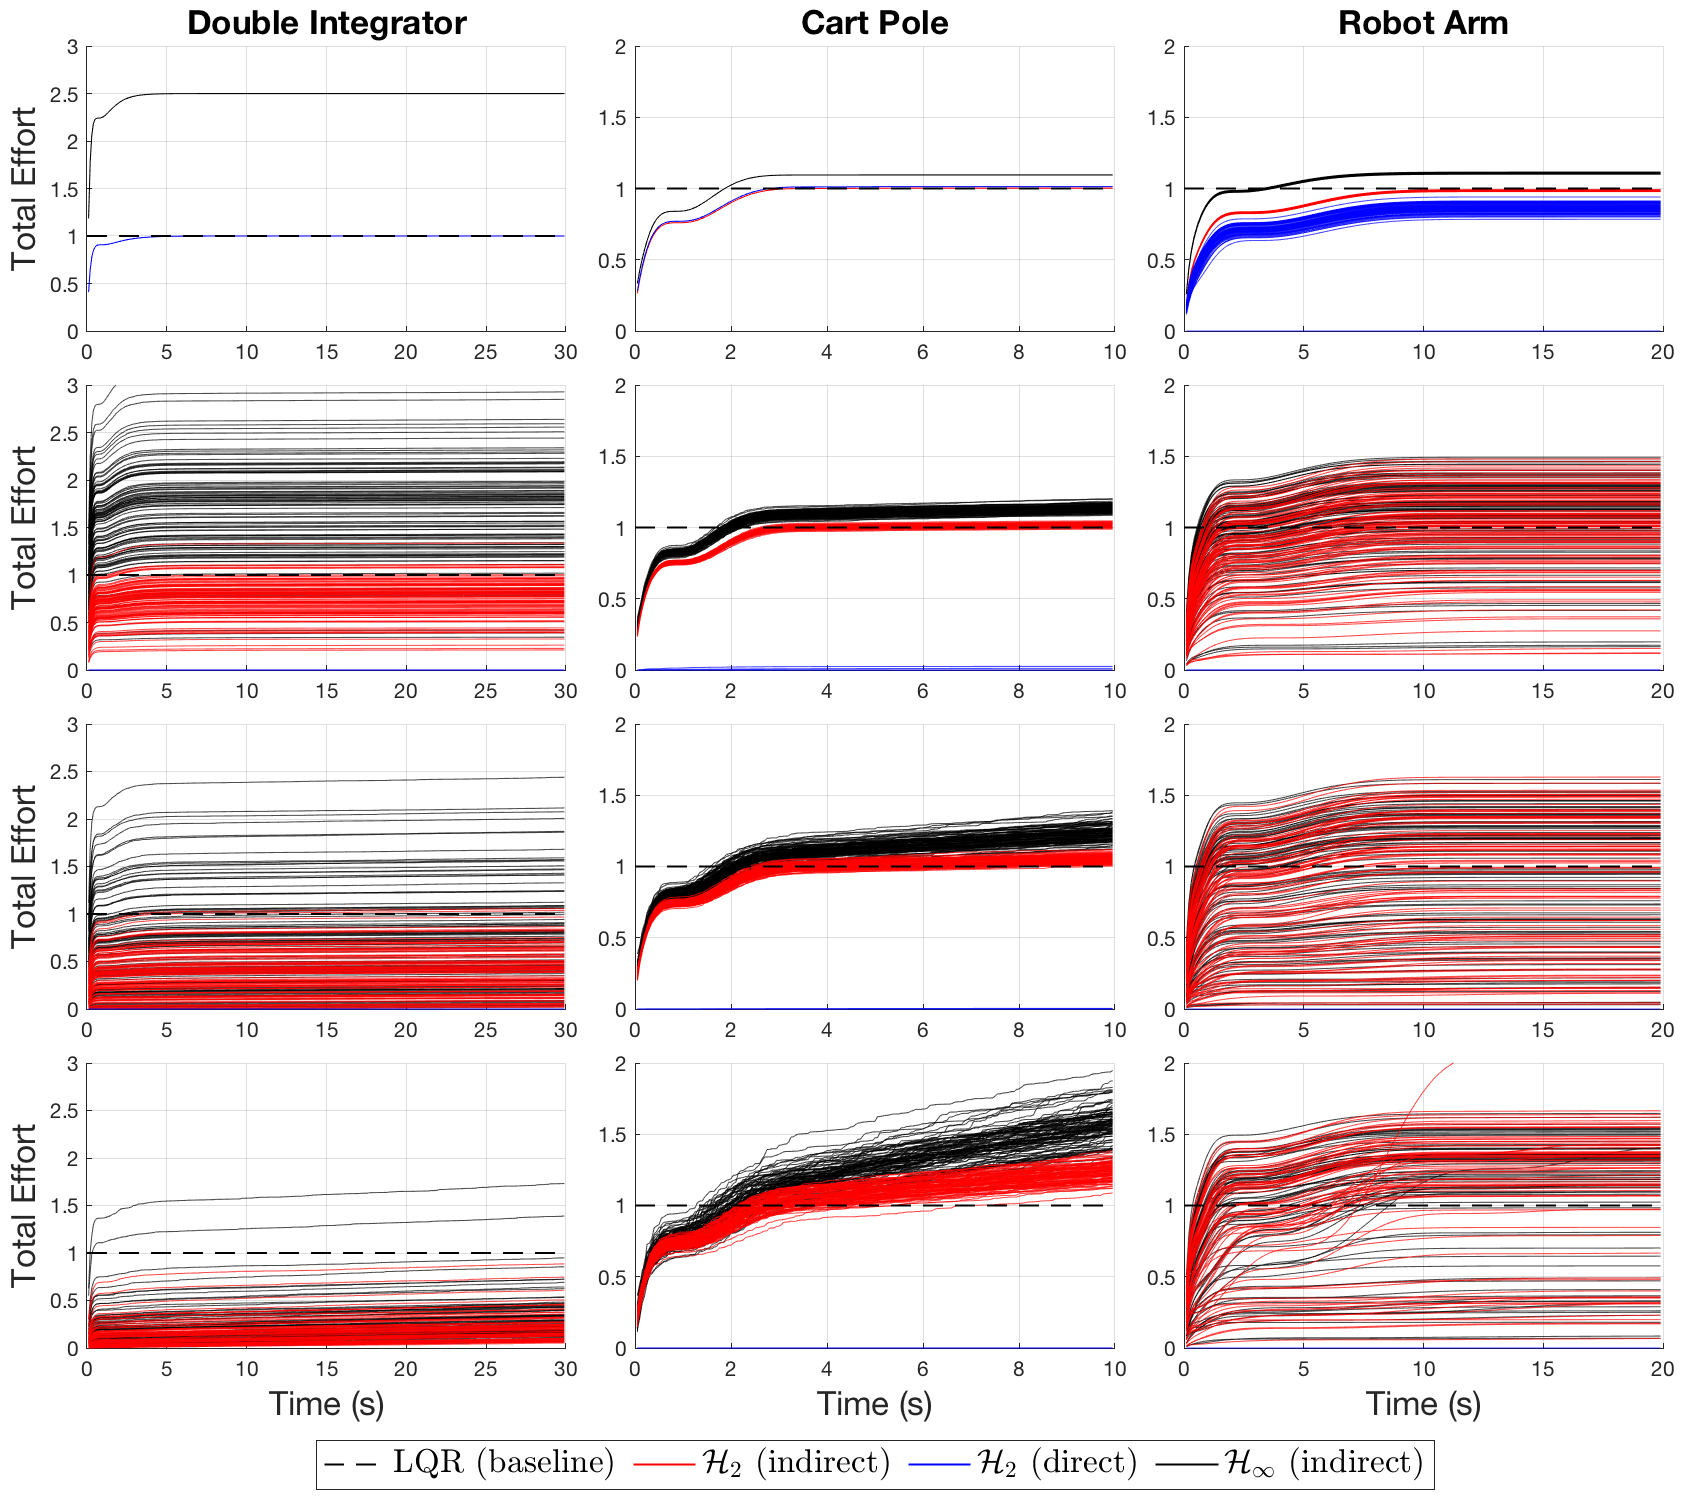
\includegraphics[width=\textwidth]{figures/noise_integrated_effort3.png}
\caption{Integrated control effort of the closed-loop generalized plant, for controllers learned from systems with measurement noise.  The rows correspond to respective scale factors of 0\%, 5\%, 10\%, and 20\%.  For each scale factor, the plots from 100 test runs are overlaid.}
\label{fig:noise_integrated_effort3}
\end{figure}

\newpage
\subsubsection{Integrated LQ Cost}
\begin{figure}[H]
\centering
	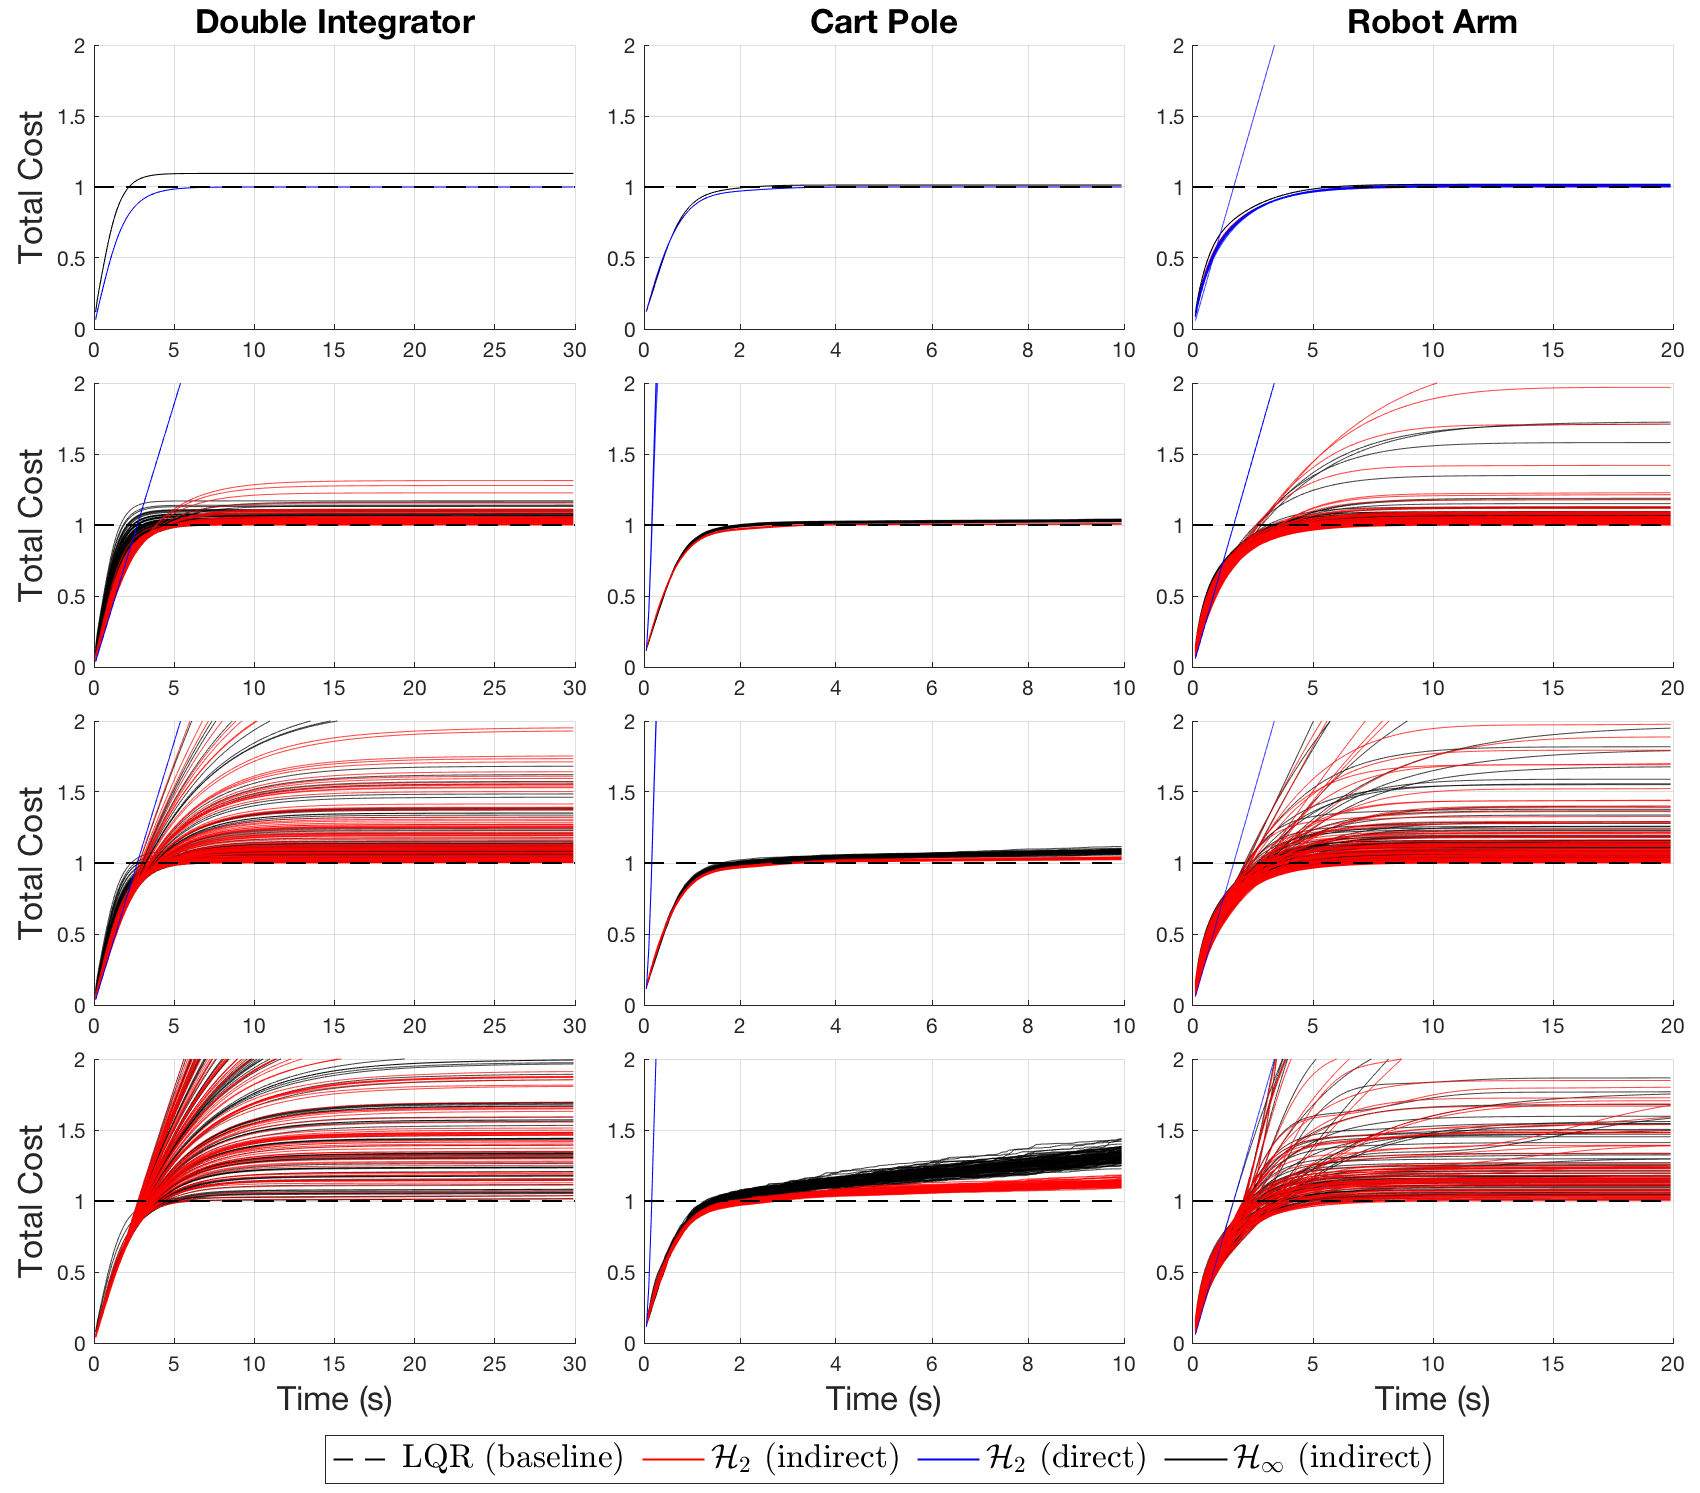
\includegraphics[width=\textwidth]{figures/noise_integrated_cost3.png}
\caption{Integrated LQ cost of the closed-loop generalized plant, for controllers learned from systems with measurement noise.  The rows correspond to respective scale factors of 0\%, 5\%, 10\%, and 20\%.  For each scale factor, the plots from 100 test runs are overlaid.}
\label{fig:noise_integrated_cost3}
\end{figure}

\newpage
\subsubsection{Overall Trends}
\underline{\textbf{Note}}: Averaged metrics shown in Figure \ref{fig:overall_trends_noise_opt_bar} are only defined for stable controllers, and may be skewed when the ``percent stable'' metric is significantly below 100\%.
\begin{figure}[H]
\centering
	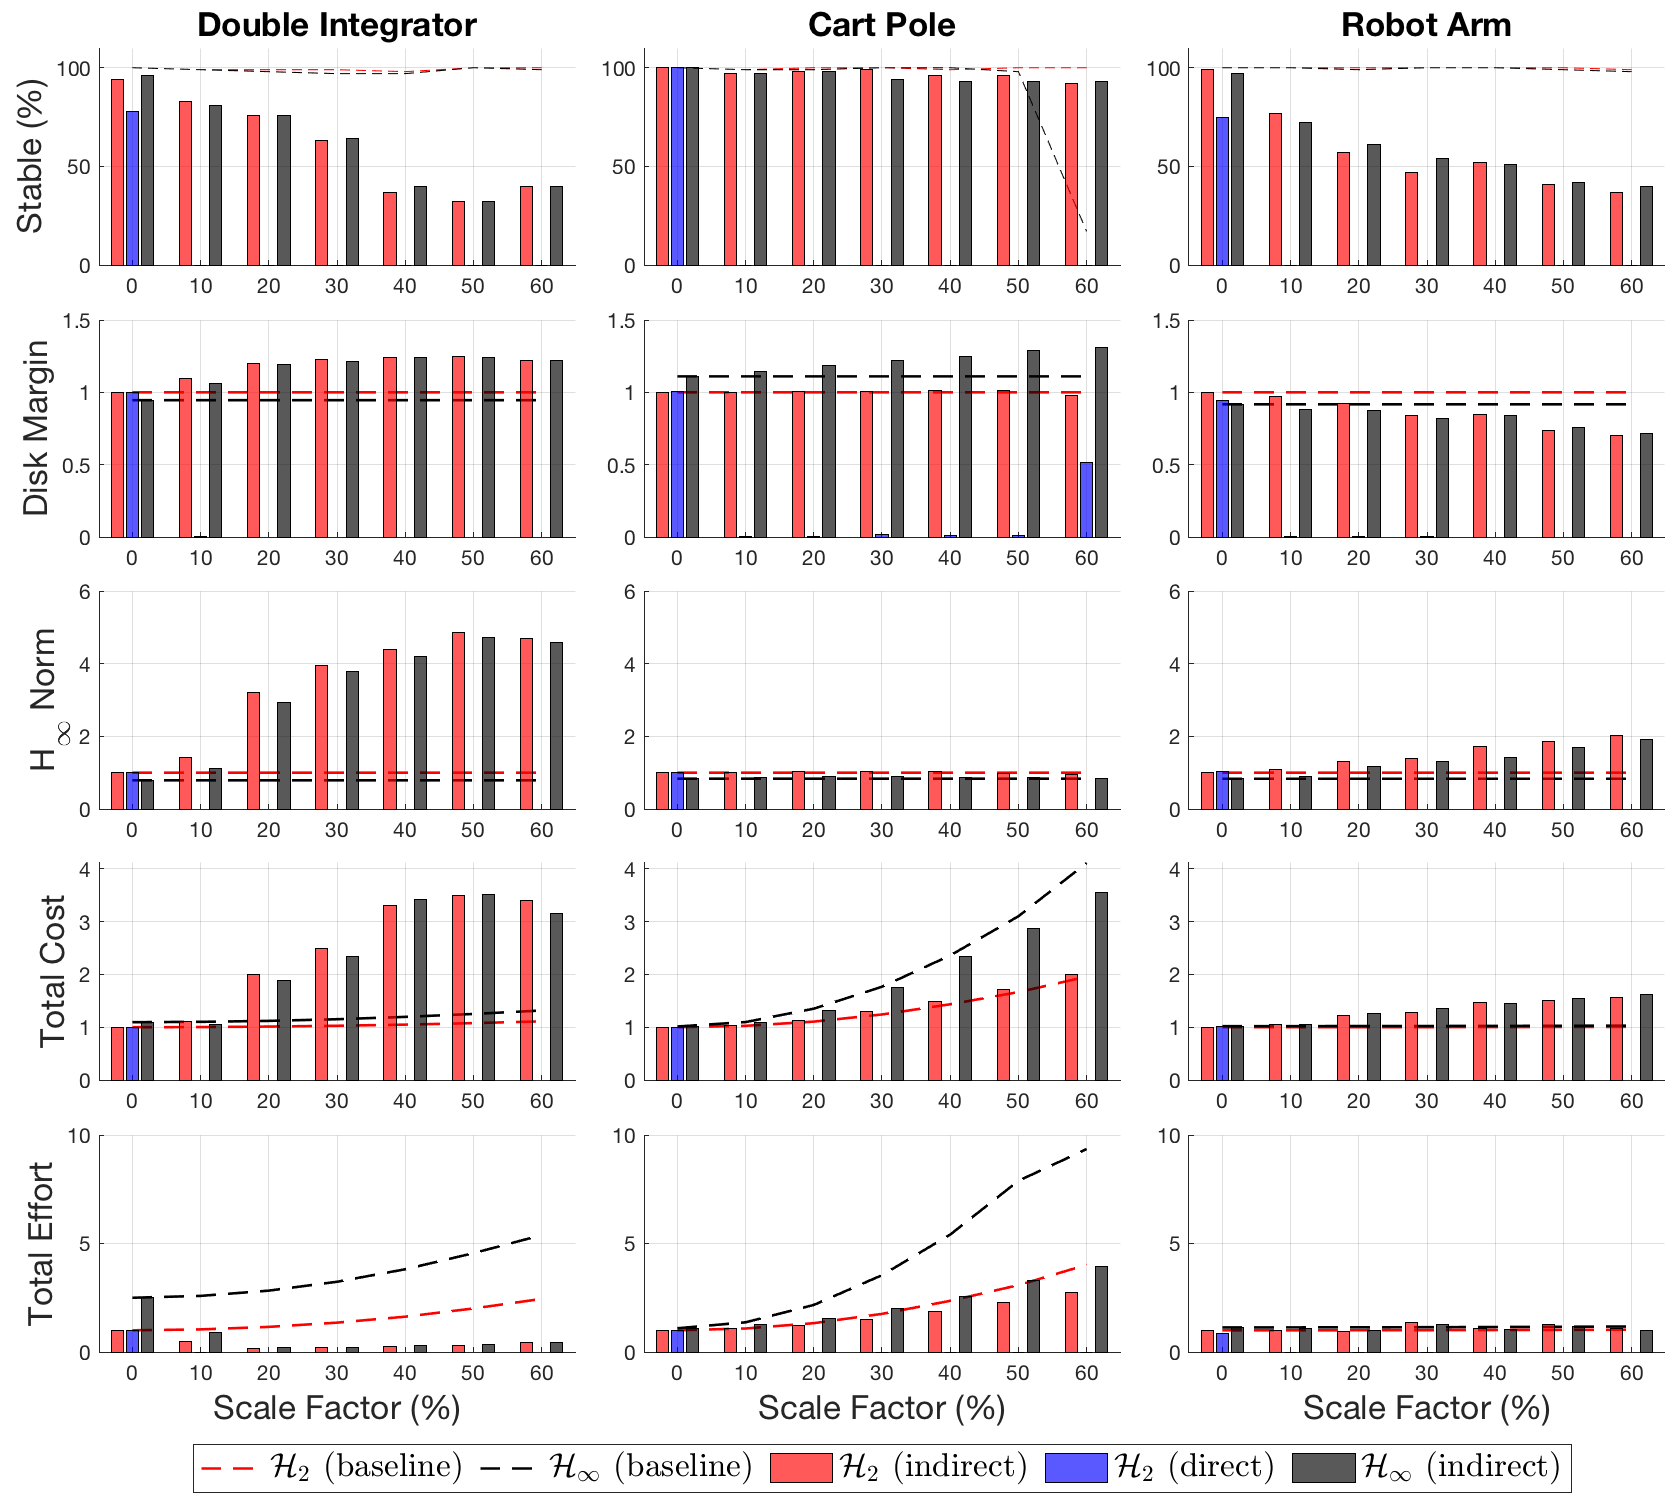
\includegraphics[width=\textwidth]{figures/overall_trends_noise_opt_bar.png}
\caption{Overall trends for scaled noise tests, comparing data-driven to baseline control approaches.  Apart from the percentage of stable controllers, all other metrics are normalized to what would be obtained by a nominal LQR/$\mathcal{H}_{2}$ feedback controller.  For each scale factor, the metrics shown are averaged across the stable test runs.}
\label{fig:overall_trends_noise_opt_bar}
\end{figure}

\newpage
\section{Test Results: Data-Driven Suboptimal $\mathcal{H}_{2}$ and $\mathcal{H}_{\infty}$}
\label{sect:results:data-driven-suboptimal}
These replace the $\mathcal{H}_{2}$-optimal LMI with the $\mathcal{H}_{2}$-suboptimal LMI described in Section \ref{sect:dataDrivenH2Suboptimal}.
\subsection{Parameter Uncertainty}
\subsubsection{Singular Values}
\begin{figure}[H]
\centering
	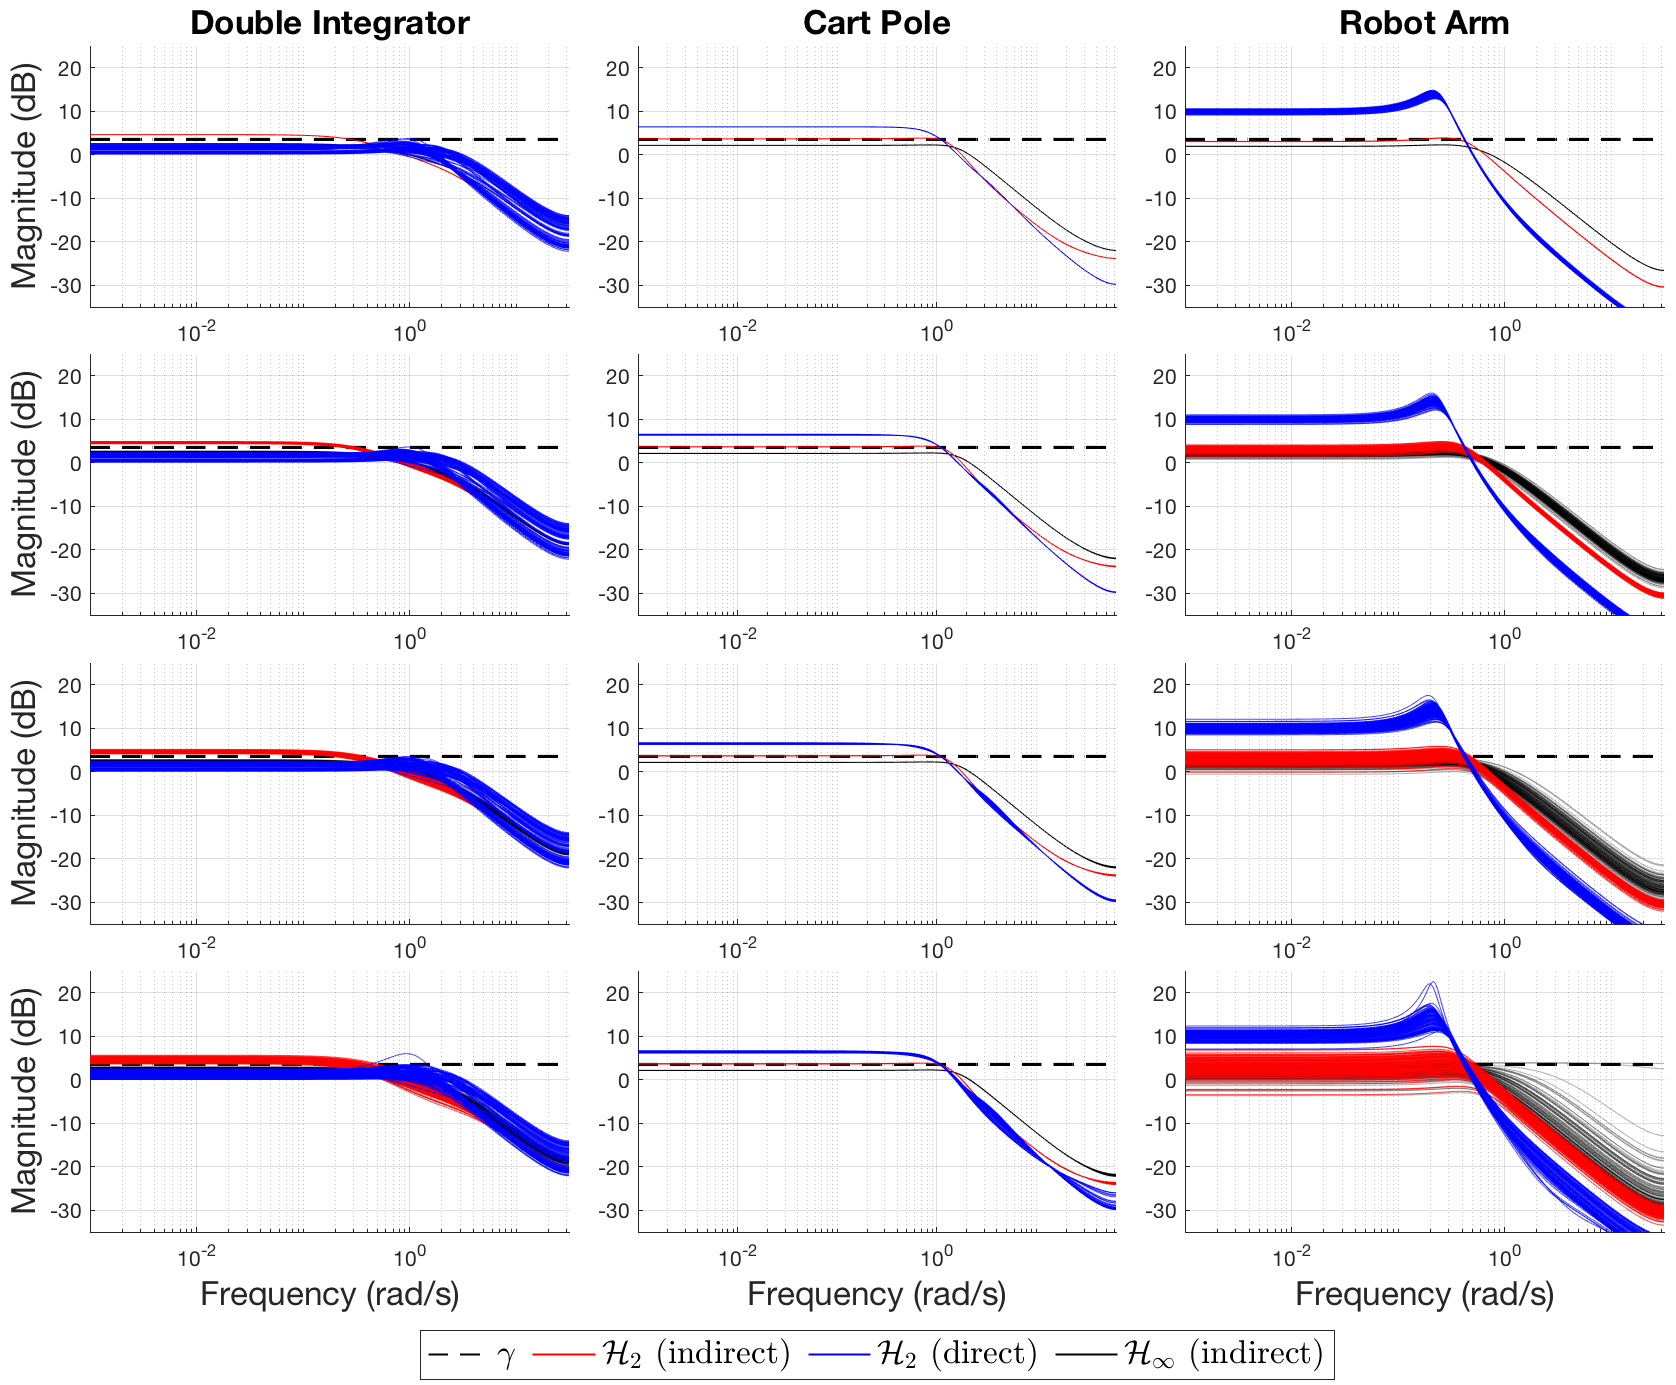
\includegraphics[width=\textwidth]{figures/uncertainty_singular_values4_s.png}
\caption{Maximum singular values of the closed-loop generalized plant, for controllers learned from systems with single-parameter uncertainty.  The rows correspond to respective scale factors of 0\%, 5\%, 10\%, and 20\%.  For each scale factor, the plots from 100 test runs are overlaid.}
\label{fig:uncertainty_singular_values4_s}
\end{figure}

\newpage
\subsubsection{Integrated Control Effort}
\begin{figure}[H]
\centering
	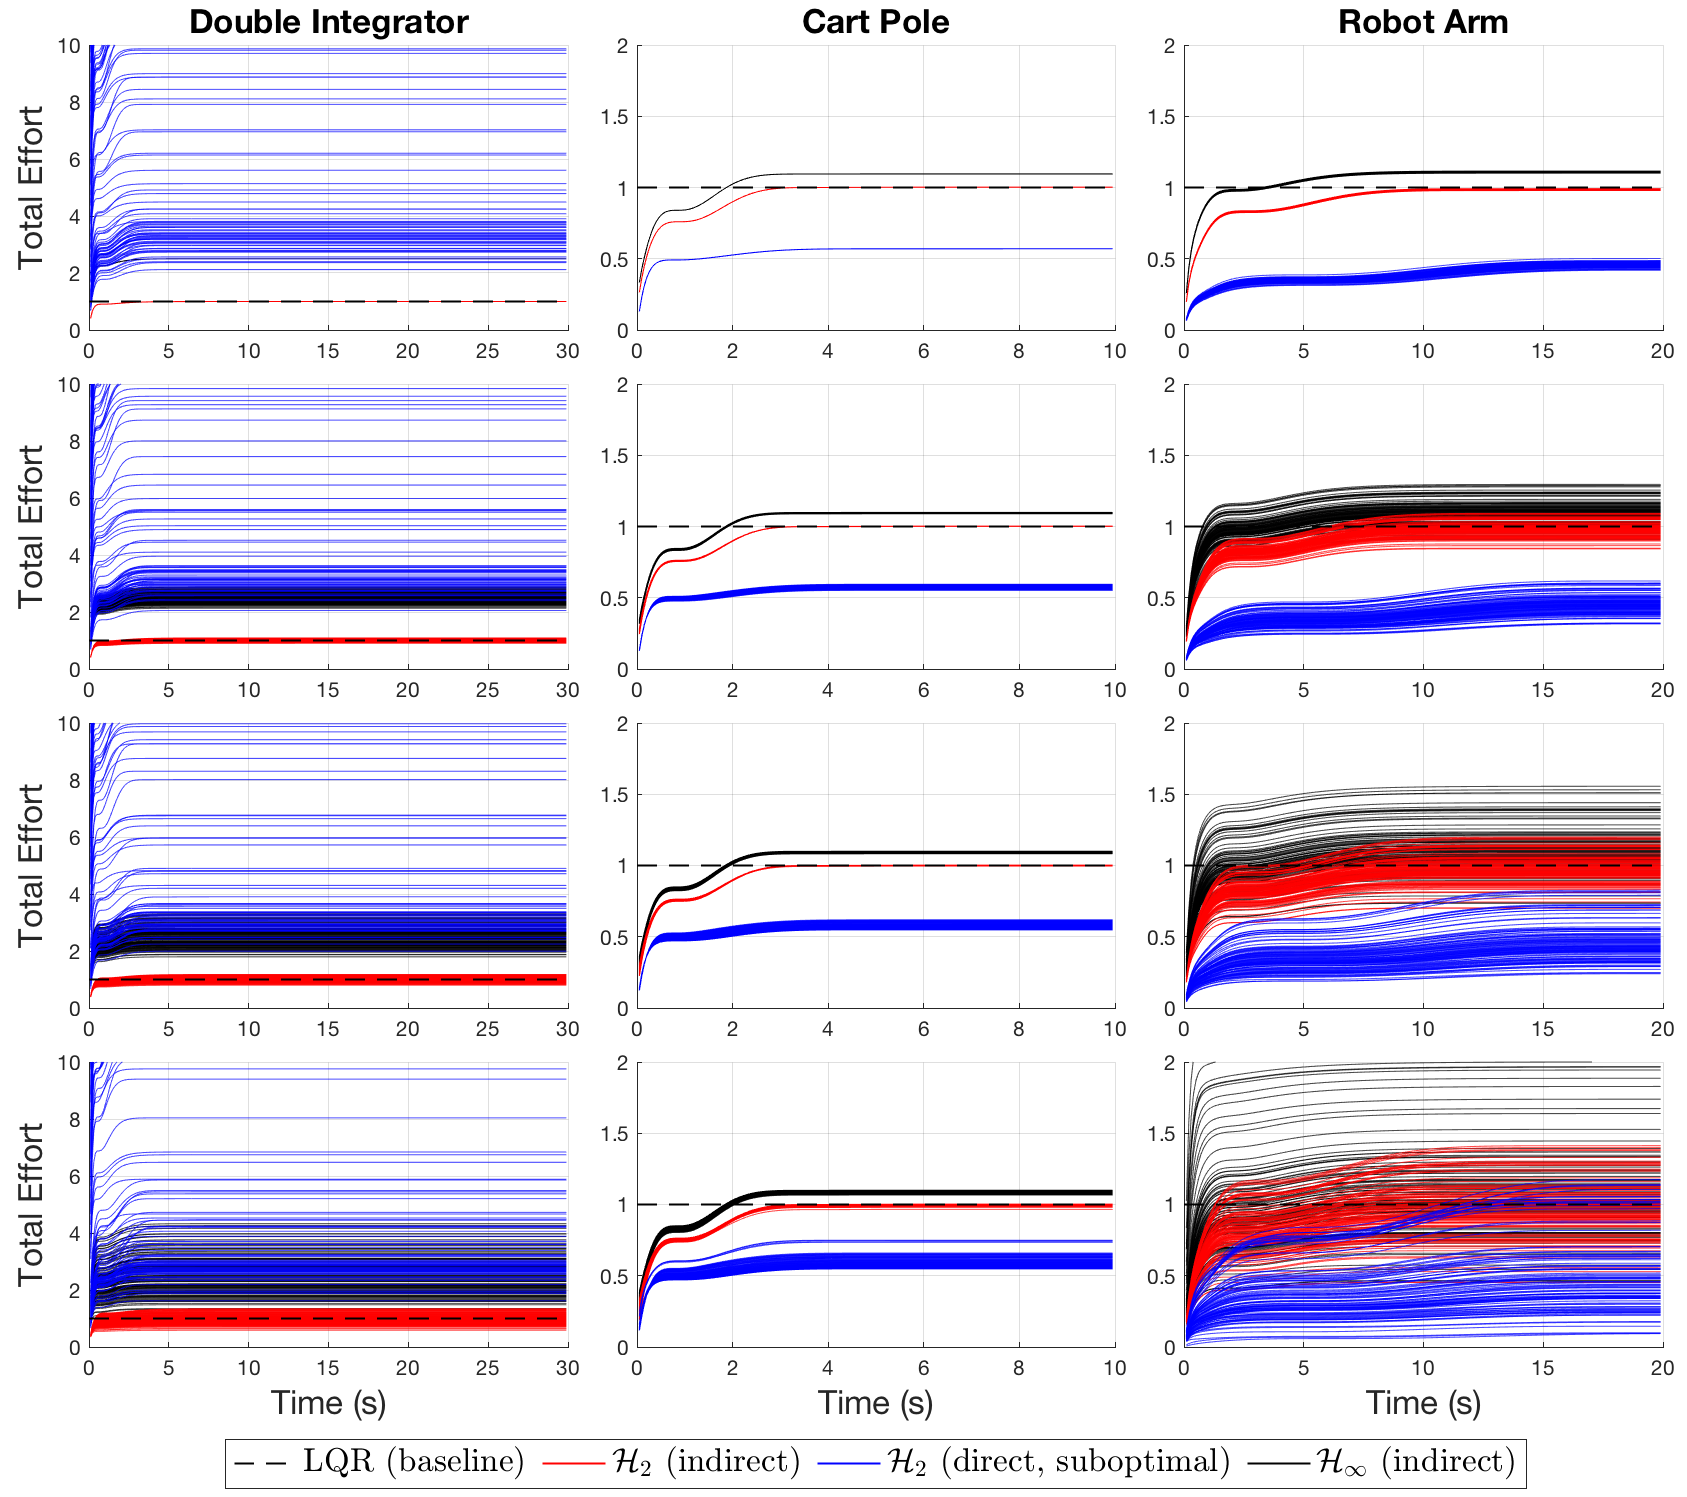
\includegraphics[width=\textwidth]{figures/uncertainty_integrated_effort4_s.png}
\caption{Integrated control effort of the closed-loop generalized plant, for controllers learned from systems with single-parameter uncertainty.  The rows correspond to respective scale factors of 0\%, 5\%, 10\%, and 20\%.  For each scale factor, the plots from 100 test runs are overlaid.}
\label{fig:uncertainty_integrated_effort4_s}
\end{figure}

\newpage
\subsubsection{Integrated LQ Cost}
\begin{figure}[H]
\centering
	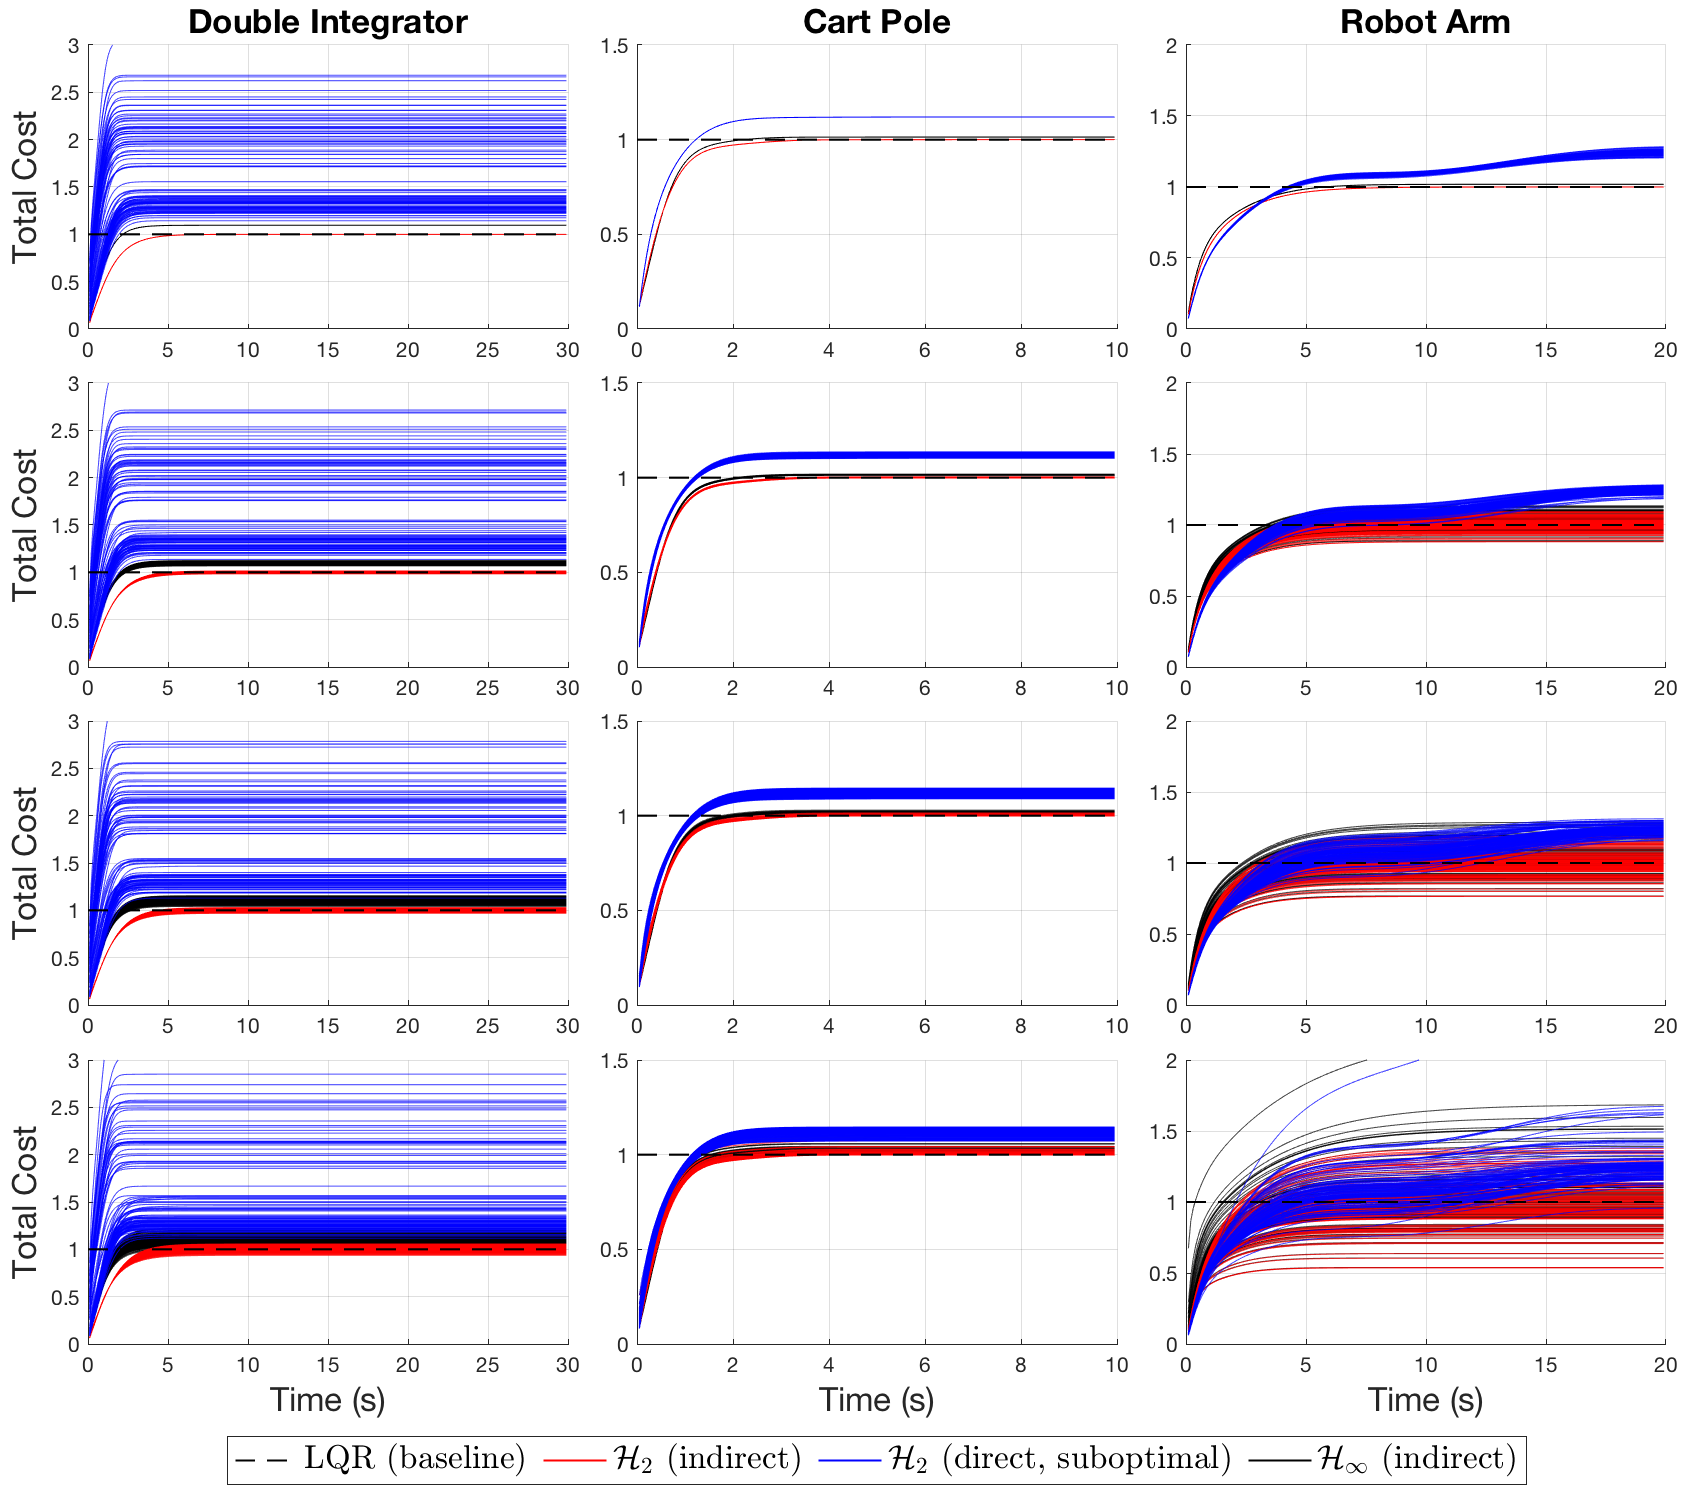
\includegraphics[width=\textwidth]{figures/uncertainty_integrated_cost4_s.png}
\caption{Integrated LQ cost of the closed-loop generalized plant, for controllers learned from systems with single-parameter uncertainty.  The rows correspond to respective scale factors of 0\%, 5\%, 10\%, and 20\%.  For each scale factor, the plots from 100 test runs are overlaid.}
\label{fig:uncertainty_integrated_cost4_s}
\end{figure}

\newpage
\subsubsection{Overall Trends}
\underline{\textbf{Note}}: Averaged metrics shown in Figure \ref{fig:overall_trends_uncertainty_subopt_bar} are only defined for stable controllers, and may be skewed when the ``percent stable'' metric is significantly below 100\%.
\begin{figure}[H]
\centering
	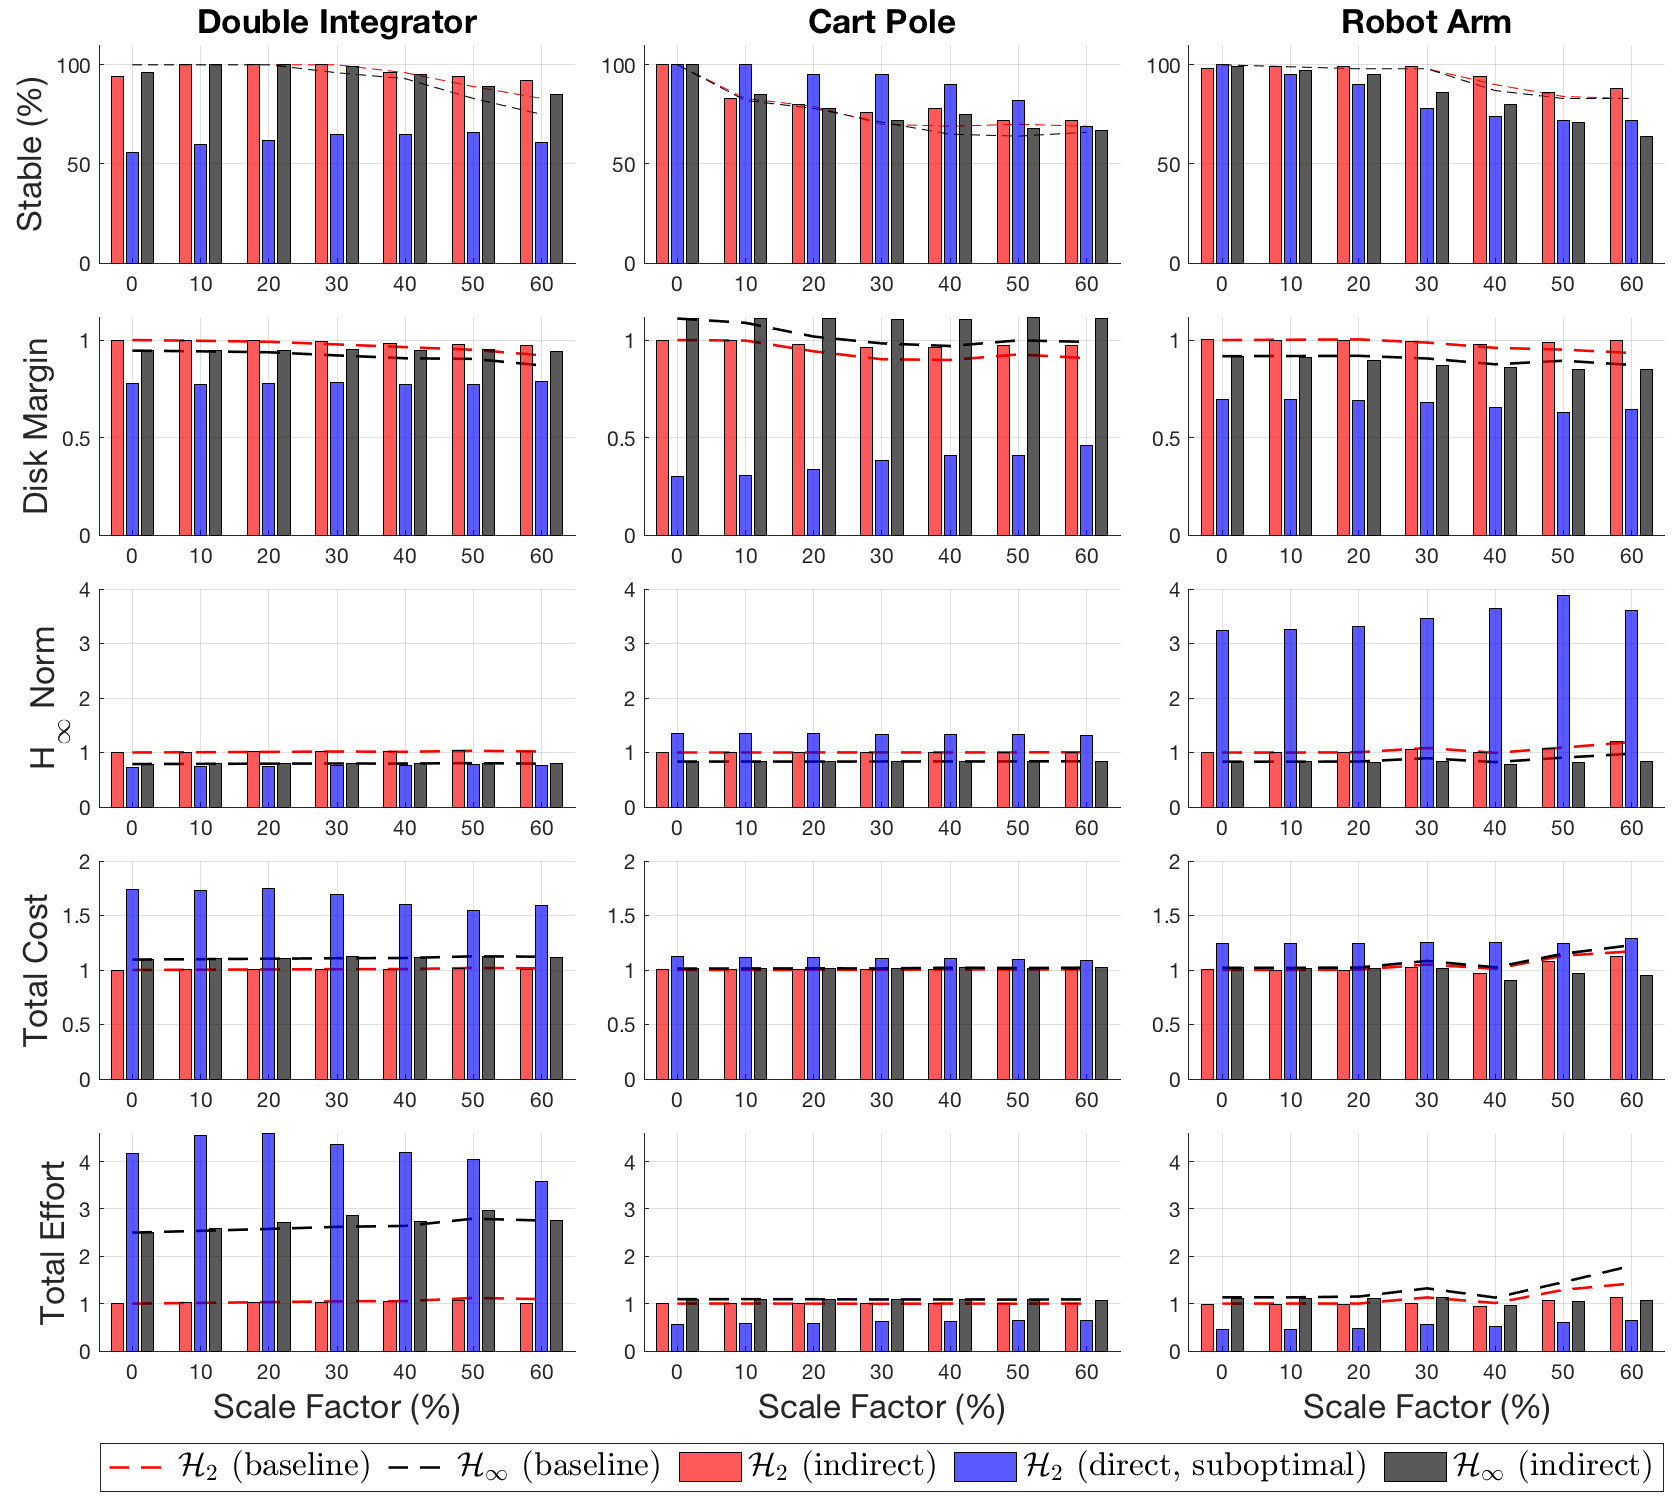
\includegraphics[width=\textwidth]{figures/overall_trends_uncertainty_subopt_bar.png}
\caption{Overall trends for scaled uncertainty tests, comparing data-driven to baseline control approaches.  Apart from the percentage of stable controllers, all other metrics are normalized to what would be obtained by a nominal LQR/$\mathcal{H}_{2}$ feedback controller.  For each scale factor, the metrics shown are averaged across the stable test runs.}
\label{fig:overall_trends_uncertainty_subopt_bar}
\end{figure}

\newpage
\subsection{Measurement Noise}
\subsubsection{Singular Values}
\begin{figure}[H]
\centering
	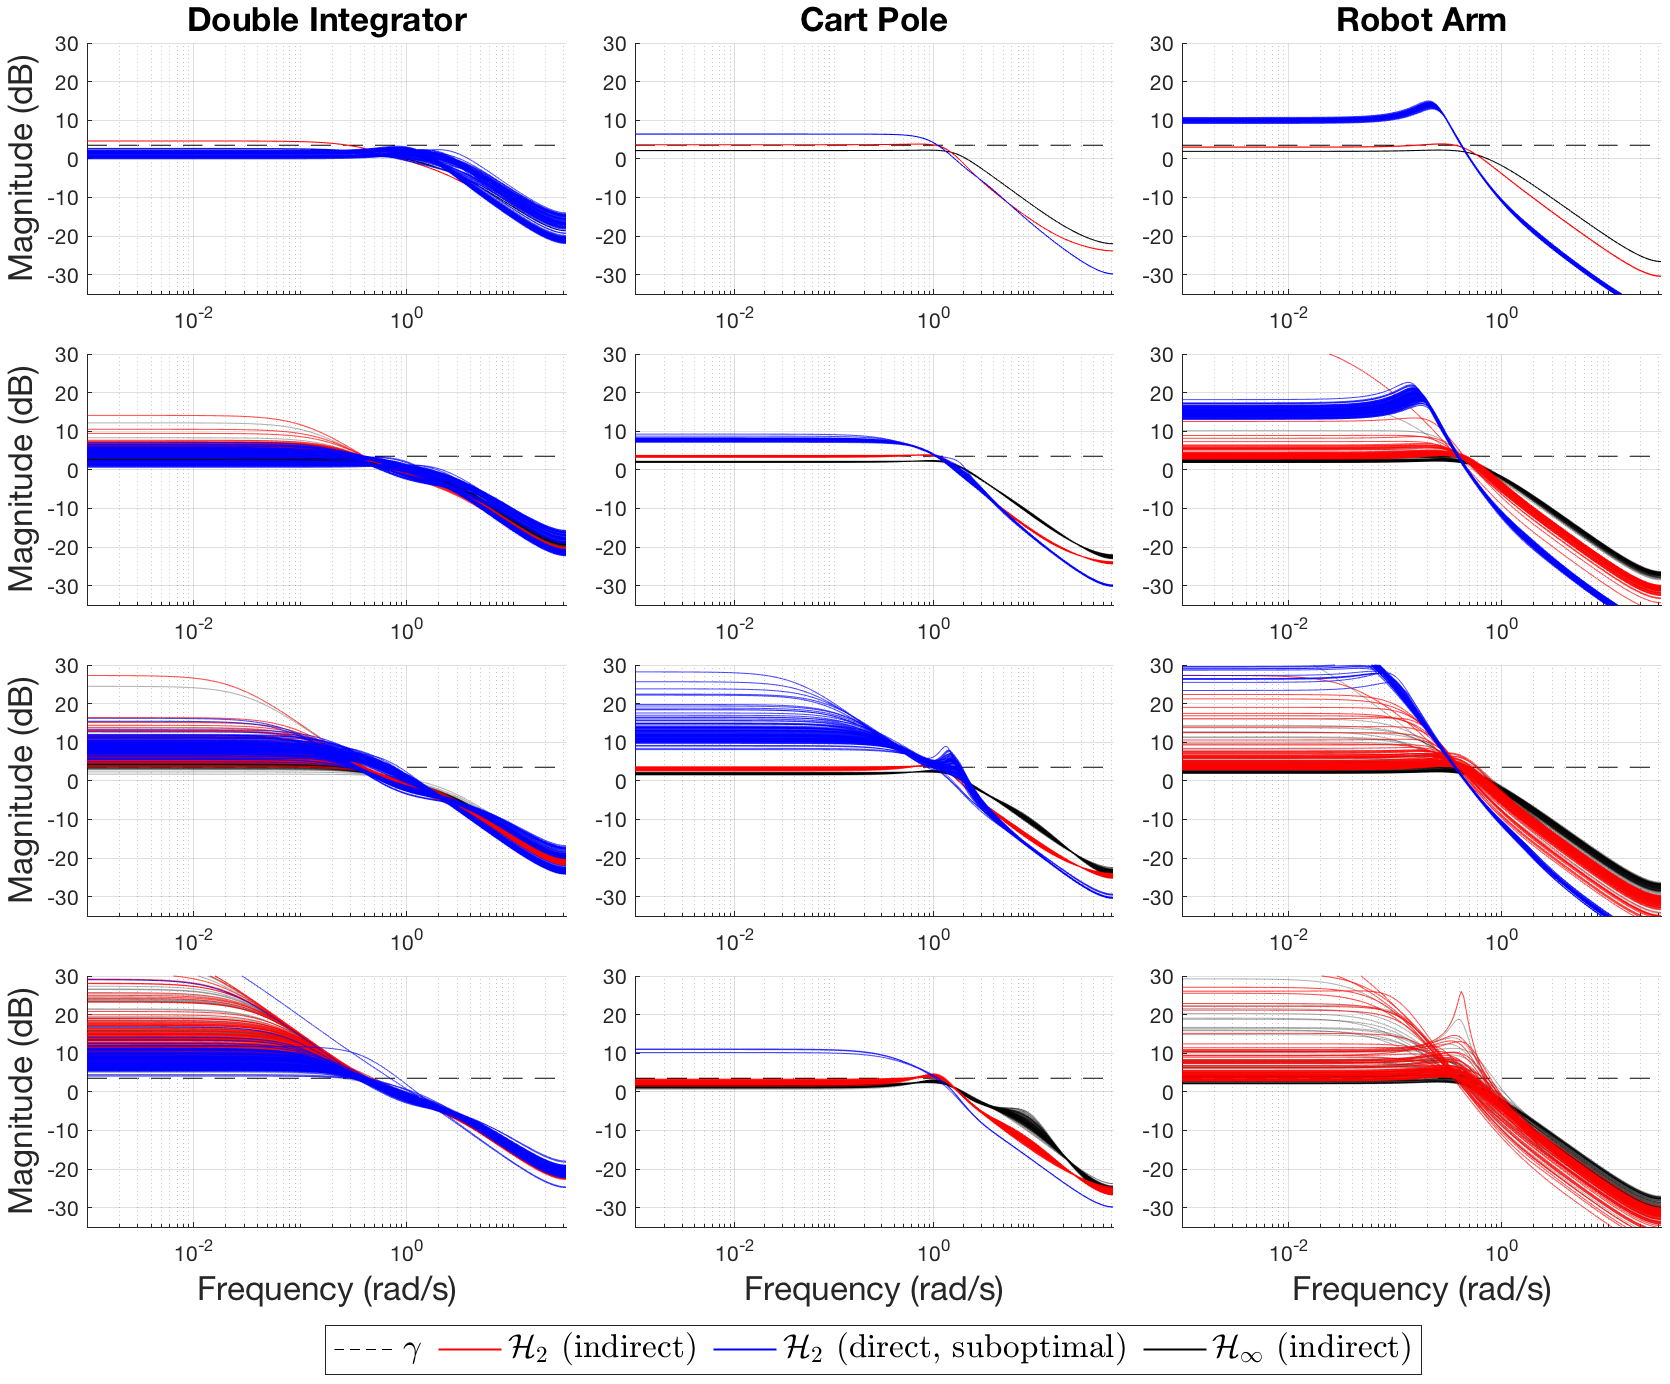
\includegraphics[width=\textwidth]{figures/noise_singular_values4_s.png}
\caption{Maximum singular values of the closed-loop generalized plant, for controllers learned from systems with measurement noise.  The rows correspond to respective scale factors of 0\%, 5\%, 10\%, and 20\%.  For each scale factor, the plots from 100 test runs are overlaid.}
\label{fig:noise_singular_values4_s}
\end{figure}

\newpage
\subsubsection{Integrated Control Effort}
\begin{figure}[H]
\centering
	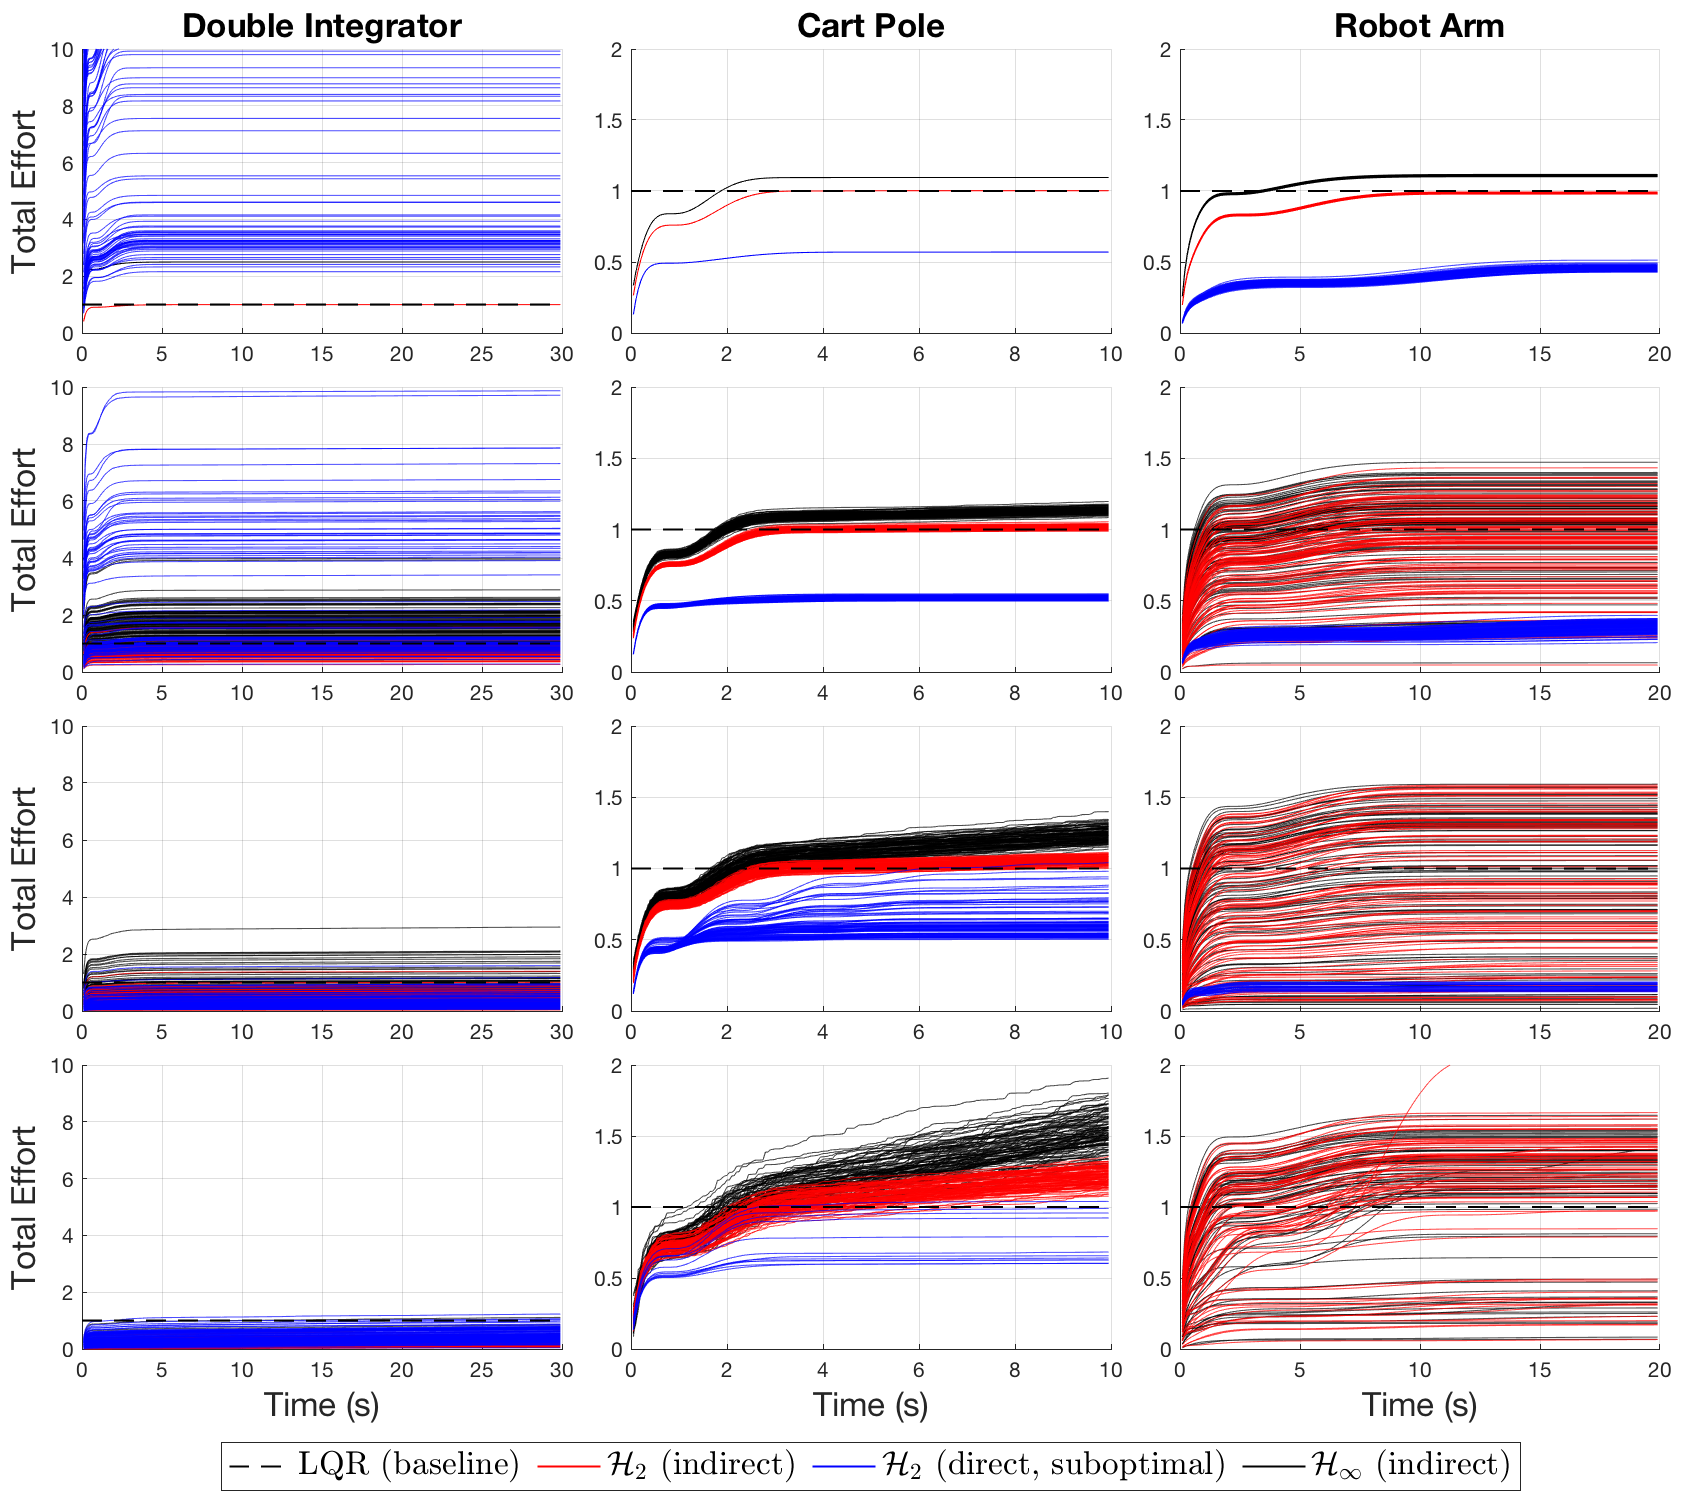
\includegraphics[width=\textwidth]{figures/noise_integrated_effort4_s.png}
\caption{Integrated control effort of the closed-loop generalized plant, for controllers learned from systems with measurement noise.  The rows correspond to respective scale factors of 0\%, 5\%, 10\%, and 20\%.  For each scale factor, the plots from 100 test runs are overlaid.}
\label{fig:noise_integrated_effort4_s}
\end{figure}

\newpage
\subsubsection{Integrated LQ Cost}
\begin{figure}[H]
\centering
	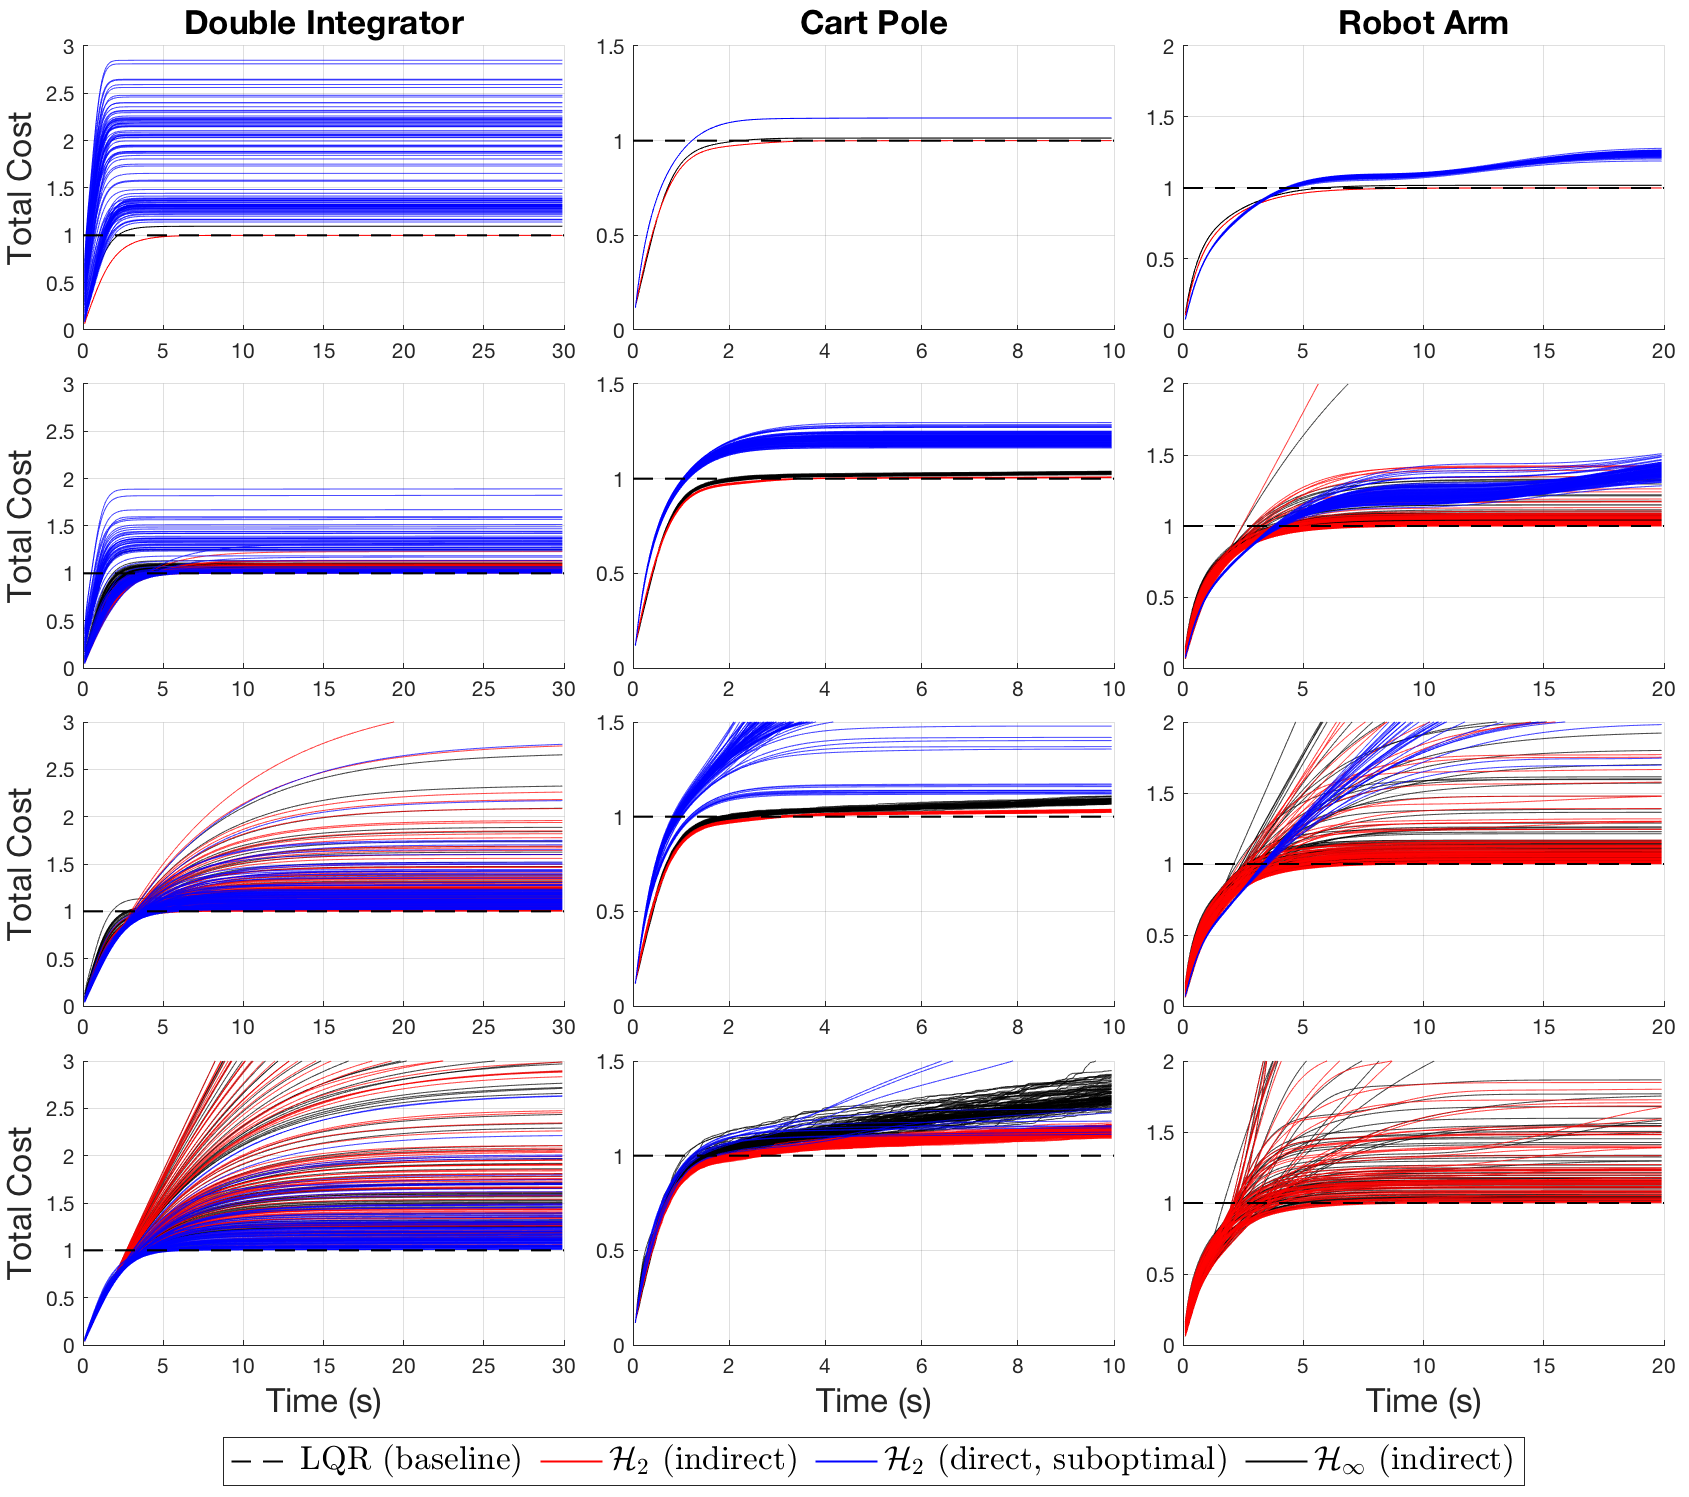
\includegraphics[width=\textwidth]{figures/noise_integrated_cost4_s.png}
\caption{Integrated LQ cost of the closed-loop generalized plant, for controllers learned from systems with measurement noise.  The rows correspond to respective scale factors of 0\%, 5\%, 10\%, and 20\%.  For each scale factor, the plots from 100 test runs are overlaid.}
\label{fig:noise_integrated_cost4_s}
\end{figure}

\newpage
\subsubsection{Overall Trends}
\underline{\textbf{Note}}: Averaged metrics shown in Figure \ref{fig:overall_trends_noise_subopt_bar} are only defined for stable controllers, and may be skewed when the ``percent stable'' metric is significantly below 100\%.
\begin{figure}[H]
\centering
	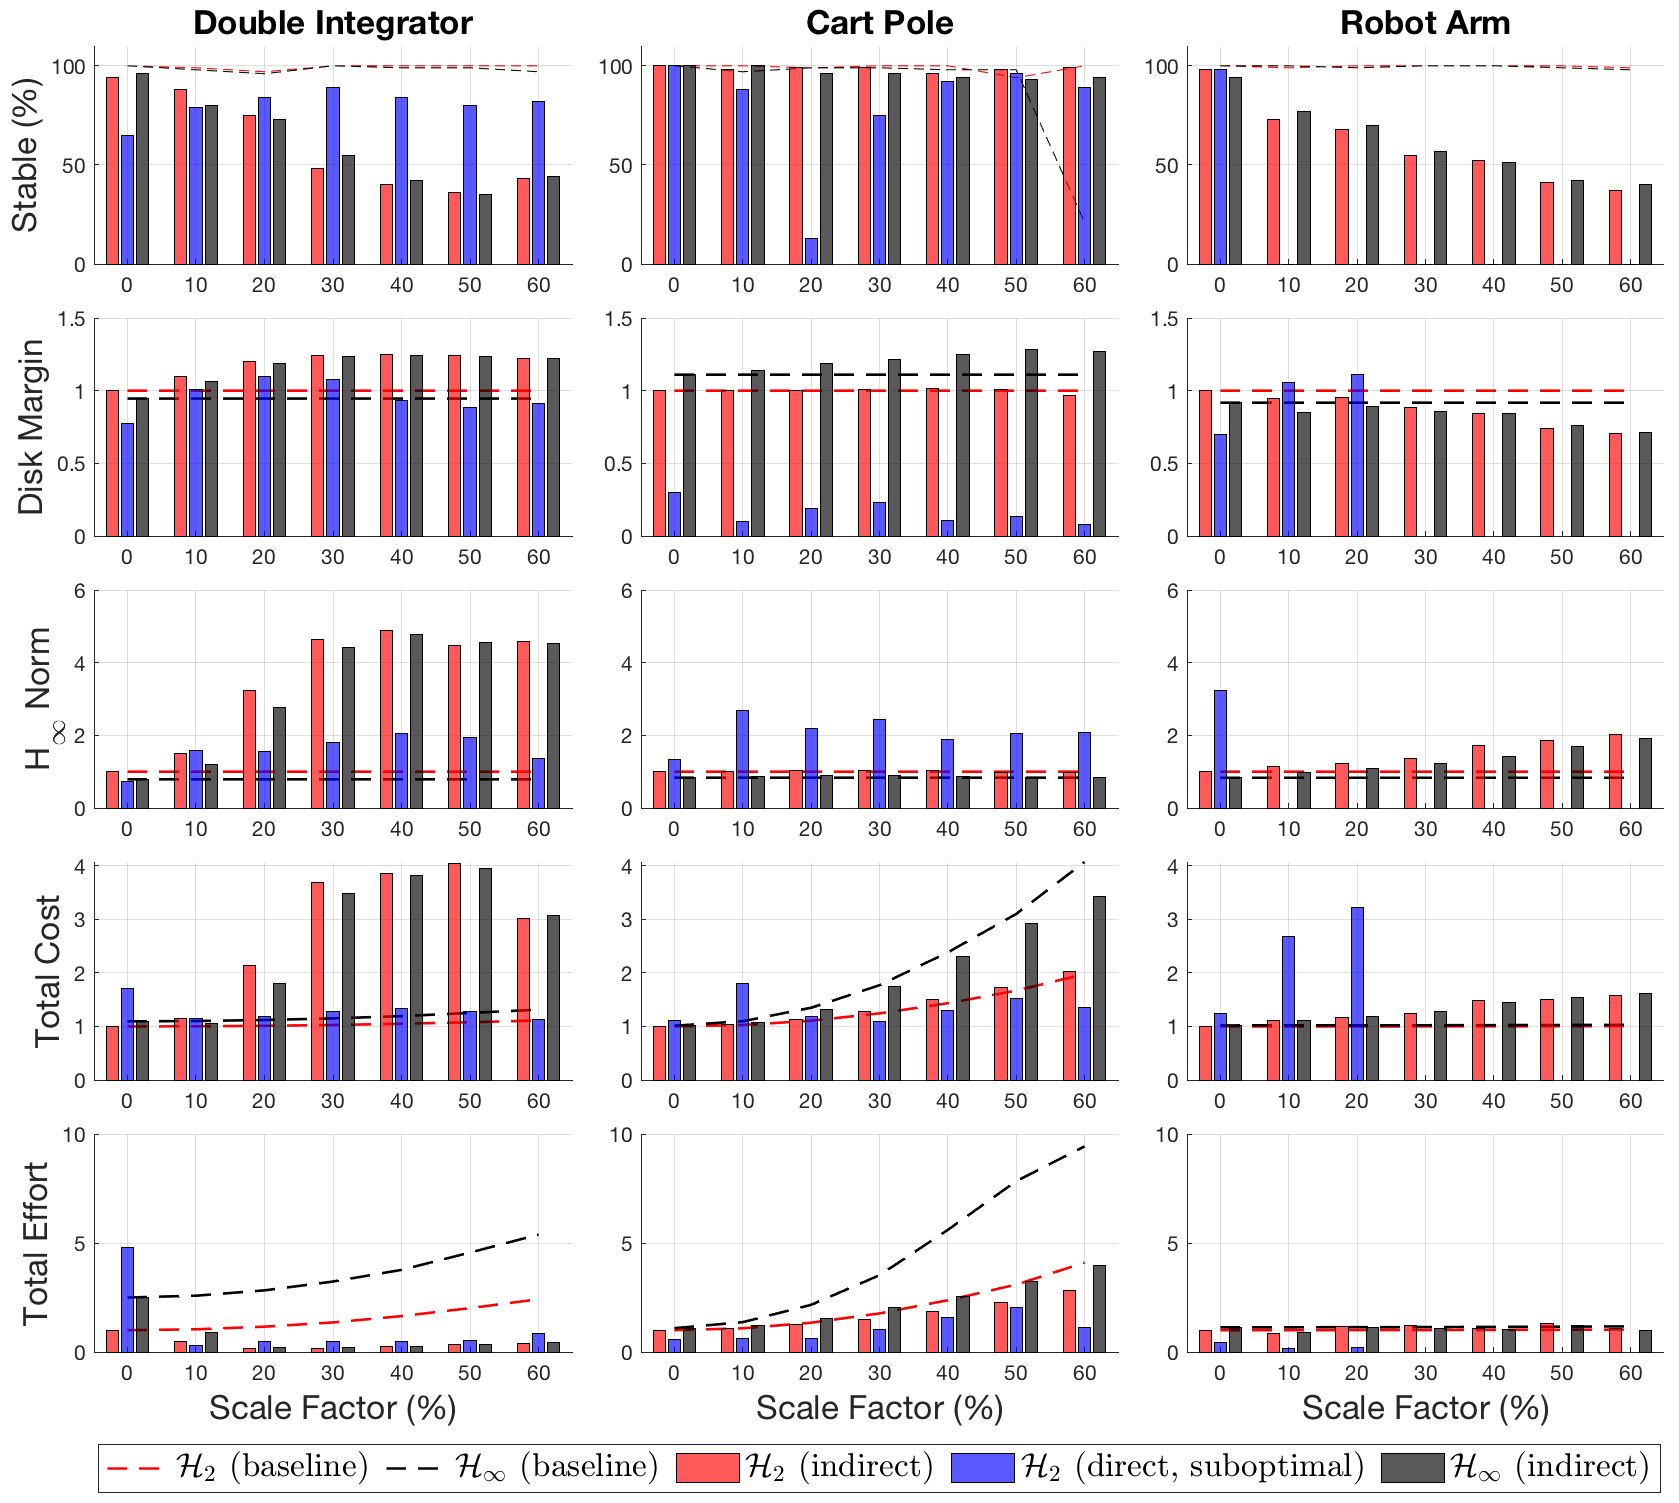
\includegraphics[width=\textwidth]{figures/overall_trends_noise_subopt_bar.png}
\caption{Overall trends for scaled noise tests, comparing data-driven to baseline control approaches.  Apart from the percentage of stable controllers, all other metrics are normalized to what would be obtained by a nominal LQR/$\mathcal{H}_{2}$ feedback controller.  For each scale factor, the metrics shown are averaged across the stable test runs.}
\label{fig:overall_trends_noise_subopt_bar}
\end{figure}

\section{Discussion}
\label{sect:results:discussion}
\subsection{Effect of Parameter Uncertainty}
Figures \ref{fig:uncertainty_singular_values3}, \ref{fig:uncertainty_integrated_effort3}, \ref{fig:uncertainty_integrated_cost3} and \ref{fig:overall_trends_uncertainty_opt_bar} illustrate the data-driven control techniques when parameter uncertainty is present (both in training data and simulation).  The variation in parameter uncertainty produced variation in all metrics.  In terms of singular values, the general loop shape was preserved, although as the uncertainty's variance was increased, the maximum singular values at higher frequencies were varied.  Note that in Figure \ref{fig:uncertainty_singular_values3}, the dotted black line represents the $\mathcal{H}_{\infty}$-optimal disturbance attenuation gain.  The $\mathcal{H}_{2}$ controllers are expected to be slightly above this line, and the $\mathcal{H}_{\infty}$ controllers are expected to be at or below it.  For the robot arm in particular, direct data-driven $\mathcal{H}_{2}$ control produced several marginally stable controllers, even for the nominal model, and this occurred more frequently as the scale factor was increased.

Note that in Figures \ref{fig:uncertainty_integrated_effort3} and \ref{fig:uncertainty_integrated_cost3}, the total cost and effort are scaled by the infinite-horizon LQR cost achieved without parameter uncertainty or noise.  The $\mathcal{H}_{2}$ controllers are expected to achieve this performance exactly, and the $\mathcal{H}_{\infty}$ control performance depends on the plant model (see Figure \ref{fig:baseline_integrated_cost}).  From these figures, the cart pole's performance is degraded far less than the double integrator and robot arm, which both see increased variation spreading roughly 5-10 times higher; this may be due to the specific coupling of training policies and plant dynamics.  Specifically, the cart pole has open-loop imaginary poles and will naturally oscillate.  Conversely, the open-loop double integrator and robot arm have real poles and will not naturally oscillate.  It seems that, for non-oscillatory systems, the quality of training data is more adversely affected by uncertainty/noise.  Future work could investigate whether an adjusted (or potentially closed-loop) training policy could yield any improvement.  For example, training could induce oscillations that sweep across relevant frequencies.

Figure \ref{fig:overall_trends_uncertainty_opt_bar} illustrates the overall trends for this test.  Note that rows 2-5 are normalized to the baseline LQR control, and are thus not absolute.  These should be interpreted as the performance of the data-driven approaches relative to the LQ optimal regulator on a system without uncertainty.

In terms of the fraction of stabilizing controllers (per 100 runs), all data-driven methods saw a decrease from 100\% down to 80\% or less as the scale factor increased.  Note that the dotted ``baseline'' lines also trend downward because the baseline controllers (when applied to the full system) eventually reach a point where nominal performance is lost due to the effect of model uncertainty.

The remaining metrics are relatively constant, though it should be noted once again these are only computed for the fraction of controllers that are stable.  What can be said is that, for those which were stable, the robustness metrics were relatively constant despite higher uncertainty.  This could be because of the training data is not providing enough information to adequately characterize the off-nominal system.  Because the training policy was held constant across all tests, there could conceivably be a shift in plant dynamics that is effectively unaccounted for during training.

\subsection{Effect of Measurement Noise}
Figures \ref{fig:noise_singular_values3}, \ref{fig:noise_integrated_effort3}, \ref{fig:noise_integrated_cost3} and \ref{fig:overall_trends_noise_opt_bar} illustrate the data-driven control techniques with measurement noise (both in training and simulation).  Figures \ref{fig:noise_integrated_effort3} and \ref{fig:noise_integrated_cost3} illustrate the effect of measurement noise on the integrated performance.  Overall trends are shown in Figure \ref{fig:overall_trends_noise_opt_bar}.

In all of the plots, it is clear that the direct (LMI-based) data-driven approach did not work when the scale factor was above 10\%.  This is due to the specification of the optimization problem, which does not account for any perturbation in the data matrices.  The indirect (SVD-based) approaches do work somewhat, though their success rate is less than 100\% and trends downward significantly for both double integrator and robot arm.  The fact that the cart pole sees adequate performance from indirect data-driven control is partly due to the fact its input/output data has more information from the state dynamics than the other two systems (a pattern also seen in Figure \ref{fig:overall_trends_uncertainty_opt_bar}).  This also highlights a relative merit of indirect data-driven control: unlike the LMI-based algorithm, the SVD provides some inherent robustness to uncorrelated noise.

In examining integrated metrics, it should be noted that increasing the scale factor is expected to cause a rise in final cost/effort.  Even after stabilization, the system continues to respond to noise in the feedback loop.  If the total cost was instead averaged over a long enough horizon (to estimate its infinite-horizon expected value), one would expect a decay.

\subsection{Effect of Performance Objective}
Numerical results also differ when directly-learned $\mathcal{H}_{2}$ controllers optimize a performance objective that allows some slack.  This was hypothesized to have some impact on how effective data-driven control was when uncertainty or noise was present (both in training data and regular plant operation).  To examine the effect of a suboptimal performance objective, the same scaled uncertainty/noise tests were run, but instead of solving the direct $\mathcal{H}_{2}$ control LMI given by Equation \eqref{eq:h2_lmi_dd}, the suboptimal variant given by Equation \eqref{eq:h2s_lmi_dd} was used.  Results for parameter uncertainty are plotted in Figures \ref{fig:uncertainty_singular_values4_s}, \ref{fig:uncertainty_integrated_effort4_s}, \ref{fig:uncertainty_integrated_cost4_s}, and \ref{fig:overall_trends_uncertainty_subopt_bar} and results for measurement noise are plotted in Figures \ref{fig:noise_singular_values4_s}, \ref{fig:noise_integrated_effort4_s}, \ref{fig:noise_integrated_cost4_s}, and \ref{fig:overall_trends_noise_subopt_bar}.

When subjected to scaled parameter uncertainty, the suboptimal $\mathcal{H}_{2}$ technique did produce more stable controllers than the optimal $\mathcal{H}_{2}$ technique.  However, between the two, the suboptimal versions consistently showed lower stability margins, higher $\mathcal{H}_{\infty}$ norms, and higher integrated effort/LQ cost.

It is interesting to note that the control effort used by the direct approach for cart pole and robot arm are on average half of what is used by the baseline and indirectly learned controllers, while the overall LQ cost is higher (10-15\% for the cart pole, and about 20-30\% for the robot arm).  This is a result of the suboptimal control objective, effectively causing a different relative weighting between state error and control effort.  Further work could involve additional tuning of LQ cost weights $\vb*{Q}_{x}$ and $\vb*{R}_{u}$ based on the performance of data-driven control, in order to investigate any potential improvements from their baseline values.

\chapter{Conclusions and Future Work}
\label{chap:conclusion}
\section{Summary}
In this thesis, a preliminary look at the robustness of offline data-driven LMIs was presented as a surrogate for machine learning problems whose solutions can be found via convex optimization.  These methods consisted of searches with various constraints (Lyapunov stability, $\mathcal{H}_{2}$ optimality, $\mathcal{H}_{\infty}$ optimality) which calculate static state feedback control parameters, with or without intermediate system identification.

When subjected to scaled single-parameter uncertainty, the data-driven approaches could synthesize a stable, robust controller which performed adequately on the full system.  However, this ability deteriorated as the scale factor increased.  Specific cut-off values varied across the case studies - approximately 30\% for the double integrator, 10\% for the cart pole, and 30\% for the robot arm.  For the fraction of stable controllers, robustness metrics were relatively constant as a function of scale factor.

When subjected to scaled measurement noise, the the direct LMI-based approach worked poorly, and did not work at all when the scale factor was above 10\%.  The indirect SVD-based approaches performed marginally better for double integrator and robot arm but still did not work 100\% of the time.  There is no precise cut-off, but the fraction of stable controllers trends downward as scale factor increases.  For the cart pole however, the indirect SVD-based approach did well to suppress noise and extract a linear plant model from its dynamic modes.

When adjusting the performance objective used for direct LMI-based approaches, there was a slight increase in the percentage of stabilizing controllers, although their performance varies from the LQ baseline as expected.  This had little effect on the ability to synthesize controllers from noisy training data, however.

\section{Tentative Conclusions}
While many factors are held constant (e.g. the training policy, the amount of data used for learning, the performance cost parameters) and simplifying assumptions were made (e.g., no rate limits or saturation, simplified inertial properties), it was demonstrated that the model-free data-driven approaches can tolerate low to moderate amounts of single parameter uncertainty.  Also, additive measurement noise can be handled to a certain degree only by using the indirect SVD-based approach, which inherently suppresses uncorrelated noise (data not attributable to the transient of a dynamic mode).  Thus, even when no exact solution exists to the optimization problem, the SVD-based least squares solution effectively produces a practically usable suboptimal solution.

The poor performance of data-driven LMIs with noisy data is expected based on the assumption of having perfect state feedback.  When this is not the case, the resulting problem can become non-convex to the point of infeasibility, resulting in the LMI solver returning a ``no solution'' condition, when in reality, there is likely a nearby suboptimal solution which stabilizes the system.  It seems necessary to encode some expected performance loss or expected uncertainty into the LMI, or more generally, seek to understand the optimization landscape of the control problem with respect to both stability \underline{and} various metrics of robustness.  Whether this combined search problem is computationally feasible in a data-driven/reinforcement learning paradigm is left for future work.

It was also demonstrated that, when solving for baseline $\mathcal{H}_{\infty}$-optimal control using the DGARE and bisection, the minimax/optimal value of disturbance attenuation constant $\gamma^{*}$ produced fragile feedback systems whose responses to the modeled disturbances are evenly ``spread'' throughout all frequencies.  However, by relaxing the optimality of the synthesis procedure with respect to the desired $\gamma \geq \gamma^{*}$, this effect becomes less prominent.  For all three case studies, this ``waterbed effect'' was clear when examining the frequency-dependent ``loop shape'' of the generalized plant's singular values.

\section{Additional Remarks}
Apart from the specific numerical results, several additional lessons were learned while developing this thesis.

The field of robust control, with its associated tools and techniques, is both very powerful and very mathematically involved.  However, it is heavily dependent on dynamic modeling of the uncertain system to be controlled.  Fortunately, modern software toolboxes/libraries can automate the solution to control design when transcribed as a mathematical optimization, but only when provided an accurate model of the disturbances and/or uncertainty faced by the real system.  Indeed, much of the practical work involved with robust control involves derivation of disturbance models and heuristic tuning of either control gains or cost weights used to compute control gains; in both cases, one leans heavily on domain-specific insight into the system being controlled.

By contrast, literature in some more computationally-focused aspects of control theory, including data-driven control and learning/optimization, often focuses more on theoretical aspects of algorithms (e.g. convergence properties, convexity, sample efficiency).  To this end, the case study dynamical systems used to test and verify numerical techniques are purposely simplified or generalized to omit the practical aspects of incorporating real-world effects into the system being learned/optimized.  Incorporating, for example, low-frequency parameter uncertainty or measurement noise (or uncertainty induced by state estimation) is not immediately obvious, or possibly feasible, using standard convex optimization paradigms.  Many similar problems are the subject of current research in robust learning.

When exploring the intersection between these two fields, as was initially the goal of this thesis, it is important to pick and focus on a somewhat smaller problem to benchmark.  Maintaining and tuning multiple simulators with a large number of parameters (e.g., cost weights, training policies and durations, plant inertial parameters, measurement noise models, initial conditions for simulation, disturbance models) and attempting to analyze properties empirically (e.g. using repeated-trial or Monte-Carlo type tests) can quickly overshadow the exploration of important theoretical properties.  Put another way, the efficacy and robustness of data-driven control depends on a wide range of factors, and evaluating different aspects is best done incrementally using smaller, more targeted analyses on a particular system.  For example, focusing on the cart pole for future analysis may allow comparison to known results in robustness/sensitivity \cite{leong2016understanding,bernat2020driver}.

\section{Future Work}
Several areas of this work were purposely oversimplified in the interest of time, and would be interesting to explore further.
\begin{itemize}
\item{\textbf{Loop Shaping:} The time-domain, game-theoretic solution to $\mathcal{H}_{\infty}$ control used in this work operates on a general state-space representation of the plant.  Cost and disturbance weights are constant matrices which are independent of frequency.  In order to utilize loop-shaping techniques, the plant's state-space model would need to be augmented with loop-shaping filters.  Interestingly, the data-driven equivalent of this problem was considered in \cite{berberich2022combining}, treating this augmented plant as partially known; filter dynamics are known, but the system dynamics are learned from data.  This seems like the right approach for further investigation of data-driven $\mathcal{H}_{\infty}$ and possibly the effect of state estimation on loop shape.  For example, robotic control involving frequency-dependent actuator dynamics may benefit from loop-shaping designs.
}
%
\item{\textbf{Disturbance Modeling:}
Disturbance modeling is an important aspect of robust control.  In order to leverage tools from robust control into model-free learning however, more difficult questions arise.  How much of the system is understood and/or modeled?  Can disturbances be modeled in a way which is flexible enough to incorporate new data that contradicts the \emph{a priori} model?  In the specific context of this work, one direction which should be expanded on is the effect of cost weighting matrices other than those associated with LQ performance.  It would be interesting to study how different performance and disturbance weights perform in model-based contexts vs. model-free contexts.  Perhaps higher-dimensional statistical techniques could be used to estimate disturbance bounds from gathered data.
}
%
\item{\textbf{Optimization Algorithms:}
This thesis aimed to evaluate specific offline techniques from \cite{de2019formulas} in the presence of uncertainty and noise.  But, many applications of reinforcement learning are based on the assumption of online adaptation of the objective function.  In particular, RL often involves some form of policy optimization, which can include, e.g., policy gradient methods, actor-critic methods, trust-region methods, etc.  For the LQR problem, these approaches are well-understood \cite{malik2019derivative}.  Extensions to LQG control \cite{zheng2022escaping, umenberger2022globally} and mixed $\mathcal{H}_{2}$/$\mathcal{H}_{\infty}$ control \cite{zhang2021derivative, zhang2020policy} have been investigated, but are noted as being non-convex.  Thus, future work in data-driven optimization should investigate algorithms for non-convex problems.  Similarly, optimization approaches which explicitly consider uncertainty in the problem data seem particularly relevant.  Indeed, the results of this thesis illustrate clearly that optimizing under the assumption of perfect state feedback is likely to be insufficient in scenarios with high uncertainty/noise.  Optimization algorithms which deal with uncertainty have been developed using the theoretical framework known as ``robust optimization'' \cite{soyster1973convex, ei1997robust, el1998robust, ben1999robust, ben2001lectures, ben2002robust, bertsimas2003robust, bertsimas2004price, chaerani2006modeling, joelianto5417249}.
}
%
\item{\textbf{Non-Robotic Systems:}
For the purposes of this work, robotic systems were selected for theoretical simplicity.  The practical value of data-driven robot control is somewhat limited though, as many robots are essentially a combination of rigid-body motion, vibrations, and actuation dynamics (all of which can be modeled).  While it is true the sensing can be challenging for small/low-cost systems, the use of state estimation is generally well-understood and standard practice.  (One possible counterexample is the use of cameras in the feedback loop, for robots performing complex manipulation tasks.)  Future work could instead focus on a specific problem which is known to be difficult from a control point of view, for which real-world datasets are available, and for which there are not obvious model-based solutions in practice, e.g. networked or distributed systems.  Observing patterns in singular values and evaluating mode decomposition could be a possible topic to explore for such a system.
}
\end{itemize}

\section{Source Code}
All MATLAB and LaTeX code used for this thesis can be found on Github at the following link: \url{https://github.com/josiahdelange/thesis}.


\appendix
%\titleformat{\chapter}{\normalfont\large}{Appendix \thechapter:}{1em}{} % change keyword
\renewcommand\chaptername{Appendix}
%\begin{appendices}
\chapter{Derivations for Plant Models}
\label{appendix:modeling}
\section{Double Integrator}
\label{appendix:modeling:doubleintegrator}
The double integrator is trivially simple, but its plant model can also be derived using Lagrangian dynamics.  The kinetic and potential energies of the system are
\begin{subequations}
\begin{align}
	K &= \frac{1}{2}m_{c}\dot{y}^{2}\\
	%
	U &= 0
\end{align}
\end{subequations}
The Lagrangian $L = K - U$ is thus
\begin{equation}
\begin{aligned}
	L = \frac{1}{2}m_{c}\dot{y}^{2}
\end{aligned}
\end{equation}
For generalized coordinate $q(t) = y(t)$, the following quantities are required:
\begin{subequations}
\begin{align}
\begin{split}
	\frac{d}{dt} \bigg{(} \frac{\partial L}{\partial \dot{y}} \bigg{)}
	&= \frac{d}{dt} \bigg{(} \frac{\partial}{\partial \dot{y}} \bigg{(} \frac{1}{2}m_{c}\dot{y}^{2} \bigg{)} \bigg{)}
	= \frac{d}{dt} \bigg{(} m_{c} \dot{y} \bigg{)} = m_{c} \ddot{y}
\end{split}
	\\
\begin{split}
	\frac{\partial L}{\partial y}
	&= \frac{\partial}{\partial y} \bigg{(}
	\frac{1}{2}m_{c}\dot{y}^{2}
	\bigg{)} = 0
\end{split}
\end{align}
\end{subequations}
Plugging these into \eqref{lagrange_eqn} yields
\begin{equation}
\begin{aligned}
	m_{c}\ddot{y} = f
\end{aligned}
\end{equation}
or, in terms of \eqref{manipulator_eqn},
\begin{subequations}
\begin{align}
	\vb*{M(q)} &= m_{c}\\
	%
	\vb*{C(q, \dot{q})} &= 0\\
	%
	\vb*{g}(\vb*{q}) &= 0\\
	%
	\vb*{B}_{\tau} &= 1
\end{align}
\end{subequations}

\section{Cart Pole}
\label{appendix:modeling:cartpole}
The kinetic and potential energies of the system are
\begin{subequations}
\begin{align}
	K &= \frac{1}{2}(m_{c} + m_{p})\dot{y}^{2} + \frac{1}{2}m_{p}l^{2}\dot{\theta}^{2} + m_{p}l\dot{y}\dot{\theta}cos(\theta)\\
	%
	U &= m_{p}glcos(\theta)
\end{align}
\end{subequations}
and the Lagrangian $L = K - U$ is thus
\begin{equation}
\begin{aligned}
	L &= \frac{1}{2}(m_{c} + m_{p})\dot{y}^{2} + \frac{1}{2}m_{p}l^{2}\dot{\theta}^{2}
		+ m_{p}l\dot{y}\dot{\theta}cos(\theta) -  m_{p}glcos(\theta)
\end{aligned}
\end{equation}
For generalized coordinate $q_{1}(t) = y(t)$, the following quantities are required:
\begin{subequations}
\begin{align}
\begin{split}
	\frac{d}{dt} \bigg{(} \frac{\partial L}{\partial \dot{y}} \bigg{)}
	&= \frac{d}{dt} \bigg{(} \frac{\partial}{\partial \dot{y}} \bigg{(}
	\frac{1}{2}(m_{c} + m_{p})\dot{y}^{2} + \frac{1}{2}m_{p}l^{2}\dot{\theta}^{2}
		+ m_{p}l\dot{y}\dot{\theta}cos(\theta) -  m_{p}glcos(\theta)
	\bigg{)} \bigg{)}
	\\
	&= \frac{d}{dt} \bigg{(}
	(m_{c} + m_{p})\dot{y} + m_{p}l\dot{\theta}cos(\theta)
	\bigg{)}
	\\
	&= (m_{c} + m_{p})\ddot{y} + m_{p}l\ddot{\theta}cos(\theta) - m_{p}l\dot{\theta}sin(\theta)
\end{split}
	\\
\begin{split}
	\frac{\partial L}{\partial y}
	&= \frac{\partial}{\partial y} \bigg{(}
	\frac{1}{2}(m_{c} + m_{p})\dot{y}^{2} + \frac{1}{2}m_{p}l^{2}\dot{\theta}^{2}
		+ m_{p}l\dot{y}\dot{\theta}cos(\theta) - m_{p}glcos(\theta)
	\bigg{)}
	\\
	&= 0
\end{split}
\end{align}
\end{subequations}
For generalized coordinate $q_{2}(t) = \theta(t)$, the following quantities are required:
\begin{subequations}
\begin{align}
\begin{split}
	\frac{d}{dt} \bigg{(} \frac{\partial L}{\partial \dot{\theta}} \bigg{)}
	&= \frac{d}{dt} \bigg{(} \frac{\partial}{\partial \dot{\theta}} \bigg{(}
	\frac{1}{2}(m_{c} + m_{p})\dot{y}^{2} + \frac{1}{2}m_{p}l^{2}\dot{\theta}^{2}
		+ m_{p}l\dot{y}\dot{\theta}cos(\theta) -  m_{p}glcos(\theta)
	\bigg{)} \bigg{)}
	\\
	&= \frac{d}{dt} \bigg{(}
	\frac{1}{2}m_{p}l^{2}\dot{\theta}^{2} + m_{p}l\dot{y}\dot{\theta}cos(\theta)
	\bigg{)}
	\\
	&= m_{p}l\ddot{y}cos(\theta) - m_{p}l\dot{y}\dot{\theta}sin(\theta) + m_{p}l^{2}\ddot{\theta}
\end{split}
	\\
\begin{split}
	\frac{\partial L}{\partial \theta}
	&= \frac{\partial}{\partial \theta} \bigg{(}
	m_{p}l\dot{y}\dot{\theta}cos(\theta) - m_{p}glcos(\theta)
	 \bigg{)}
	\\
	&= -m_{p}l\dot{y}\dot{\theta}sin(\theta) - m_{p}glsin(\theta)
\end{split}
\end{align}
\end{subequations}
Plugging each of these into \eqref{lagrange_eqn} yields
\begin{subequations}
\begin{align}
	f &= (m_{c} + m_{p})\ddot{y} + m_{p}l\ddot{\theta}cos(\theta) - m_{p}l\dot{\theta}sin(\theta)\\
	0 &= m_{p}l\ddot{y}cos(\theta) + m_{p}l^{2}\ddot{\theta} + m_{p}glsin(\theta)
\end{align}
\end{subequations}
or, in terms of the manipulator equation \eqref{manipulator_eqn},
\begin{subequations}
\begin{align}
	\vb*{M(q)} &= \begin{bmatrix}
		m_{c} + m_{p} & m_{p}lcos(\theta)\\
		m_{p}lcos(\theta) & m_{p}l^{2}\\
	\end{bmatrix}\\
	%
	\vb*{C(q, \dot{q})} &= \begin{bmatrix}
		0 & -m_{p}l\dot{\theta}sin(\theta)\\
		0 & 0\\
	\end{bmatrix}\\
	%
	\vb*{g}(\vb*{q}) &= \begin{bmatrix} 0 \\ m_{p}glsin(\theta) \end{bmatrix}\\
	%
	\vb*{B}_{\tau} &= \begin{bmatrix} 1\\ 0 \end{bmatrix}
\end{align}
\end{subequations}

\section{Robot Arm}
\label{appendix:modeling:robotarm}
The kinetic and potential energies of the system are
\begin{subequations}
\begin{align}
\begin{split}
	K &= \frac{1}{2}(m_{1} + m_{2})l_{1}^{2}\dot{\theta_{1}}^{2} +
	\frac{1}{2}m_{2}l_{2}^{2}(\dot{\theta_{1}}^{2} + \dot{\theta_{2}}^{2})
	\\
	& + \frac{1}{2}m_{2} \bigg{(} l_{2}^{2}\dot{\theta_{1}}^{2}
	+ 2l_{1}l_{2}\dot{\theta_{1}}^{2}cos(\theta_{2}) + 2l_{1}l_{2}\dot{\theta_{1}}\dot{\theta_{2}}cos(\theta_{2})
	+ 2l_{2}^{2}\dot{\theta_{1}}\dot{\theta_{2}} \bigg{)}
\end{split}
	\\
	U &= m_{1}gl_{1}cos(\theta_{1}) + m_{2}gl_{1}cos(\theta_{1}) + m_{2}gl_{2}cos(\theta_{1} + \theta_{2})
\end{align}
\end{subequations}
The Lagrangian $L = K - U$ is thus
\begin{equation}
\begin{aligned}
	L &= \frac{1}{2}(m_{1} + m_{2})l_{1}^{2}\dot{\theta_{1}}^{2} +
	\frac{1}{2}m_{2}l_{2}^{2}(\dot{\theta_{1}}^{2} + \dot{\theta_{2}}^{2})
	\\
	& + \frac{1}{2}m_{2} \bigg{(} l_{2}^{2}\dot{\theta_{1}}^{2}
	+ 2l_{1}l_{2}\dot{\theta_{1}}^{2}cos(\theta_{2}) + 2l_{1}l_{2}\dot{\theta_{1}}\dot{\theta_{2}}cos(\theta_{2})
	+ 2l_{2}^{2}\dot{\theta_{1}}\dot{\theta_{2}} \bigg{)}
	\\
	& - m_{1}gl_{1}cos(\theta_{1}) - m_{2}gl_{1}cos(\theta_{1}) - m_{2}gl_{2}cos(\theta_{1} + \theta_{2})
\end{aligned}
\end{equation}
For generalized coordinate $q_{1}(t) = \theta_{1}(t)$, the following quantities are required:
\begin{subequations}
\begin{align}
\begin{split}
	\frac{d}{dt} \bigg{(} \frac{\partial L}{\partial \dot{\theta}_{1}} \bigg{)}
	&= \frac{d}{dt} \bigg{(} \frac{\partial}{\partial \dot{\theta}_{1}} \bigg{(}
	\frac{1}{2}(m_{1} + m_{2})l_{1}^{2}\dot{\theta_{1}}^{2} +
	\frac{1}{2}m_{2}l_{2}^{2}(\dot{\theta_{1}}^{2} + \dot{\theta_{2}}^{2})
	\\
	& + \frac{1}{2}m_{2} \bigg{(} l_{2}^{2}\dot{\theta_{1}}^{2}
	+ 2l_{1}l_{2}\dot{\theta_{1}}^{2}cos(\theta_{2}) + 2l_{1}l_{2}\dot{\theta_{1}}\dot{\theta_{2}}cos(\theta_{2})
	+ 2l_{2}^{2}\dot{\theta_{1}}\dot{\theta_{2}} \bigg{)}
	\\
	& - m_{1}gl_{1}cos(\theta_{1}) - m_{2}gl_{1}cos(\theta_{1}) - m_{2}gl_{2}cos(\theta_{1} + \theta_{2})
	\bigg{)} \bigg{)}
	\\
	&= \frac{d}{dt} \bigg{(}
	(m_{1} + m_{2})l_{1}^{2}\dot{\theta_{1}} +
	m_{2}l_{2}^{2}(\dot{\theta_{1}} + \dot{\theta_{2}})
	+ 2m_{2}l_{1}l_{2}\dot{\theta_{1}}cos(\theta_{2}) + m_{2}l_{1}l_{2}\dot{\theta_{2}}cos(\theta_{2})
	\bigg{)}
	\\
	&= (m_{1} + m_{2})l_{1}^{2}\ddot{\theta_{1}} +
	m_{2}l_{2}^{2}(\ddot{\theta_{1}} + \ddot{\theta_{2}})
	+ 2m_{2}l_{1}l_{2}\ddot{\theta_{1}}cos(\theta_{2})\\
	&- 2m_{2}l_{1}l_{2}\dot{\theta_{1}}\dot{\theta_{2}}sin(\theta_{2})
	+ m_{2}l_{1}l_{2}\ddot{\theta_{2}}cos(\theta_{2})
	- m_{2}l_{1}l_{2}\dot{\theta_{2}}^{2}sin(\theta_{2})
\end{split}
	\\
\begin{split}
	\frac{\partial L}{\partial \theta_{1}} &=
	\frac{\partial}{\partial \theta_{1}} \bigg{(}
	\frac{1}{2}(m_{1} + m_{2})l_{1}^{2}\dot{\theta_{1}}^{2} +
	\frac{1}{2}m_{2}l_{2}^{2}(\dot{\theta_{1}}^{2} + \dot{\theta_{2}}^{2})
	\\
	& + \frac{1}{2}m_{2} \bigg{(} l_{2}^{2}\dot{\theta_{1}}^{2}
	+ 2l_{1}l_{2}\dot{\theta_{1}}^{2}cos(\theta_{2}) + 2l_{1}l_{2}\dot{\theta_{1}}\dot{\theta_{2}}cos(\theta_{2})
	+ 2l_{2}^{2}\dot{\theta_{1}}\dot{\theta_{2}} \bigg{)}
	\\
	& - m_{1}gl_{1}cos(\theta_{1}) - m_{2}gl_{1}cos(\theta_{1}) - m_{2}gl_{2}cos(\theta_{1} + \theta_{2})
	\bigg{)}
	\\	
	&= (m_{1} + m_{2})gl_{1}cos(\theta_{1}) + m_{2}gl_{2}sin(\theta_{1} + \theta_{2})
\end{split}
\end{align}
\end{subequations}
For generalized coordinate $q_{2}(t) = \theta_{2}(t)$, the following quantities are required:
\begin{subequations}
\begin{align}
\begin{split}
	\frac{d}{dt} \bigg{(} \frac{\partial L}{\partial \dot{\theta}_{2}} \bigg{)}
	&= \frac{d}{dt} \bigg{(} \frac{\partial}{\partial \dot{\theta}_{2}} \bigg{(}
	\frac{1}{2}(m_{1} + m_{2})l_{1}^{2}\dot{\theta_{1}}^{2} +
	\frac{1}{2}m_{2}l_{2}^{2}(\dot{\theta_{1}}^{2} + \dot{\theta_{2}}^{2})
	\\
	& + \frac{1}{2}m_{2} \bigg{(} l_{2}^{2}\dot{\theta_{1}}^{2}
	+ 2l_{1}l_{2}\dot{\theta_{1}}^{2}cos(\theta_{2}) + 2l_{1}l_{2}\dot{\theta_{1}}\dot{\theta_{2}}cos(\theta_{2})
	+ 2l_{2}^{2}\dot{\theta_{1}}\dot{\theta_{2}} \bigg{)}
	\\
	& - m_{1}gl_{1}cos(\theta_{1}) - m_{2}gl_{1}cos(\theta_{1}) - m_{2}gl_{2}cos(\theta_{1} + \theta_{2}
	\bigg{)} \bigg{)}
	\\
	&= \frac{d}{dt} \bigg{(}
	m_{2}l_{2}^{2}(\dot{\theta_{1}} + \dot{\theta_{2}}) + m_{2}l_{1}l_{2}\dot{\theta_{1}}cos(\theta_{2})
	\bigg{)}
	\\
	&= m_{2}l_{2}^{2}(\ddot{\theta_{1}} + \ddot{\theta_{2}})
	+ m_{2}l_{1}l_{2}\ddot{\theta_{1}}cos(\theta_{2})
	- m_{2}l_{1}l_{2}\dot{\theta_{1}}\dot{\theta_{2}}sin(\theta_{2})
\end{split}
	\\
\begin{split}
	\frac{\partial L}{\partial \theta_{2}} &=
	\frac{\partial}{\partial \theta_{2}} \bigg{(}
	\frac{1}{2}(m_{1} + m_{2})l_{1}^{2}\dot{\theta_{1}}^{2} +
	\frac{1}{2}m_{2}l_{2}^{2}(\dot{\theta_{1}}^{2} + \dot{\theta_{2}}^{2})
	\\
	& + \frac{1}{2}m_{2} \bigg{(} l_{2}^{2}\dot{\theta_{1}}^{2}
	+ 2l_{1}l_{2}\dot{\theta_{1}}^{2}cos(\theta_{2}) + 2l_{1}l_{2}\dot{\theta_{1}}\dot{\theta_{2}}cos(\theta_{2})
	+ 2l_{2}^{2}\dot{\theta_{1}}\dot{\theta_{2}} \bigg{)}
	\\
	& - m_{1}gl_{1}cos(\theta_{1}) - m_{2}gl_{1}cos(\theta_{1}) - m_{2}gl_{2}cos(\theta_{1} + \theta_{2})
	\bigg{)}
	\\	
	&= -m_{2}l_{1}l_{2}\dot{\theta_{1}}^{2}sin(\theta_{2})
	- m_{2}l_{1}l_{2}\dot{\theta_{1}}\dot{\theta_{2}}sin(\theta_{2})
	+ m_{2}gl_{2}sin(\theta_{1} + \theta_{2})
\end{split}
\end{align}
\end{subequations}
Plugging each of these into \eqref{lagrange_eqn} yields
\begin{subequations}
\begin{align}
\begin{split}
	\tau_{1} &= (m_{1} + m_{2})l_{1}^{2}\ddot{\theta_{1}} +
	m_{2}l_{2}^{2}(\ddot{\theta_{1}} + \ddot{\theta_{2}})
	+ 2m_{2}l_{1}l_{2}\ddot{\theta_{1}}cos(\theta_{2})
	- 2m_{2}l_{1}l_{2}\dot{\theta_{1}}\dot{\theta_{2}}sin(\theta_{2})\\
	&+ m_{2}l_{1}l_{2}\ddot{\theta_{2}}cos(\theta_{2})
	- m_{2}l_{1}l_{2}\dot{\theta_{2}}^{2}sin(\theta_{2})
	- (m_{1} + m_{2})gl_{1}cos(\theta_{1}) - m_{2}gl_{2}sin(\theta_{1} + \theta_{2})
\end{split}
	\\
\begin{split}
	\tau_{2} &= m_{2}l_{2}^{2}(\ddot{\theta_{1}} + \ddot{\theta_{2}})
	+ m_{2}l_{1}l_{2}\ddot{\theta_{1}}cos(\theta_{2})
	+ m_{2}l_{1}l_{2}\dot{\theta_{1}}^{2}sin(\theta_{2})
	- m_{2}gl_{2}sin(\theta_{1} + \theta_{2})
\end{split}
\end{align}
\end{subequations}
or, in terms of the manipulator equation \eqref{manipulator_eqn},
\begin{subequations}
\begin{align}
	\vb*{M(q)} &= \begin{bmatrix}
		(m_{1} + m_{2})l_{1}^{2} + m_{2}l_{2}^{2} + 2m_{1}l_{1}l_{2}cos(\theta_{2}) &
		m_{2}l_{2}^{2} + m_{2}l_{1}l_{2}cos(\theta_{2})\\
		m_{2}l_{2}^{2} + m_{2}l_{1}l_{2}cos(\theta_{2}) & m_{2}l_{2}^{2}
	\end{bmatrix}\\
	%
	\vb*{C(q, \dot{q})} &= \begin{bmatrix}
		-2m_{2}l_{1}l_{2}\dot{\theta_{2}}sin(\theta_{2}) & -m_{2}l_{1}l_{2}\dot{\theta_{2}}sin(\theta_{2})\\
		m_{2}l_{1}l_{2}\dot{\theta_{2}}sin(\theta_{2}) & 0\\
	\end{bmatrix}\\
	%
	\vb*{g}(\vb*{q}) &= \begin{bmatrix}
		(m_{1} + m_{2})gl_{1}cos(\theta_{1}) + m_{2}gl_{2}sin(\theta_{1} + \theta_{2})\\
		m_{2}gl_{2}sin(\theta_{1} + \theta_{2})\\
	\end{bmatrix}\\
	%
	\vb*{B}_{\tau} &= \begin{bmatrix} 1 & 0 \\ 0 & 1 \end{bmatrix}
\end{align}
\end{subequations}
\chapter{Sensitivity of Feedback Systems}
\label{appendix:sensitivity}
\section{Overview}
Consider the discrete-time unity feedback system in Figure \ref{fig:servo_mechanism}.  Controlled inputs $\vb{u}$ are calculated based on the error $\vb{e} = \vb{r} - \vb{y}$ between the reference/desired input and noisy output of $\vb{P}(z)$, and input disturbances add to them.
The variable $z = e^{j\omega}$, where $\omega$ is a real frequency, $G(z)$ denotes a discrete-time single-input single output (SISO) transfer function, and $\vb{G}(z)$ denotes a discrete multi-input multi-output (MIMO) transfer function matrix. 
\begin{figure}[H]
\centering
\resizebox{0.8\textwidth}{!}{
	% Feedback control servomechanism with disturbances
	\begin{tikzpicture}[>=stealth]
		% Coordinates
		\coordinate (orig) at (0,0);
		\coordinate (LLS1) at (1.5,0);
		\coordinate (LLK) at (3,-0.5);
		\coordinate (LLS2) at (5,0);
		\coordinate (LLP) at (5.75,-0.5);
		\coordinate (LLS3) at (8,-1.5);

		% Loop transfer function bounding box
		%\node[draw, dashed, minimum width=4.75cm, minimum height=1.5cm,
		%	anchor=south west, text width=3cm, align=center,fill=gray!4] (L) at ($(LLP.0) - (3.15,0.25)$) {};
		%\node[text width=1cm] at ($(LLP.0) + (0.3,1.5)$) {\small $\vb*{L}$};
		%\node[text width=1cm] at ($(LLS2.0) + (0.29,-0.65)$) {\small $\vb*{L}$};

		% Transfer functions
		\node[draw, fill=white, minimum width=1cm, minimum height=1cm, anchor=south west,
			text width=1cm, align=center] (P) at (LLP) {\footnotesize $\vb*{P}(z)$};
		\node[draw, fill=white, minimum width=1cm, minimum height=1cm, anchor=south west,
			text width=1cm, align=center] (C) at (LLK) {\footnotesize $\vb*{K}(z)$};

		% Sum/junctions
		\draw [fill=white] (LLS1) circle [radius=0.15cm];
		\draw [fill=white] (LLS2) circle [radius=0.15cm];
		\draw [fill=white] (LLS3) circle [radius=0.15cm];

		% Signals
		\draw[->] ($(LLS1.0) - (1.5,0)$) -- node[above]{\footnotesize $\vb*{r}$} ($(LLS1.0) - (0.15,0)$);
		\draw[->] ($(LLS1.0) + (0.15,0)$) -- node[above, pos=0.4]{\footnotesize $\vb*{e}$} ($(LLK.0) + (0,0.5)$);
		\draw[->] ($(LLK) + (1.28,0.5)$) -- node[above, pos=0.5]{\footnotesize $\vb*{u}$} ($(LLS2.0) - (0.15,0)$);
		\draw[->] ($(LLS2.0) + (0.15,0)$) -- ($(LLP.0) + (0,0.5)$);
		\draw[->] ($(LLP) + (1.28,0.5)$) -- node[above, pos=0.35]{\footnotesize $\vb*{y}$} ($(LLP.0) + (3.5,0.5)$);
		\draw[->] ($(LLS3.0) + (0,1.5)$) -- ($(LLS3.0) + (0,0.15)$);
		\draw[-] ($(LLS3.0) - (0.15, 0)$) |- ($(LLK.0) - (0,1)$);
		\draw[->] ($(LLK.0) - (0,1)$) -| node[left, pos=0.95]{\footnotesize $-$} ($(LLS1.0) - (0,0.15)$);
		\draw[->] ($(LLS2.0) + (0,1)$) -- node[above, pos=0]{\footnotesize $\vb*{d}$} ($(LLS2.0) + (0,0.15)$);
		\draw[->] ($(LLS3.0) + (1.15,0)$) -- node[right, pos=0]{\footnotesize $\vb*{n}$} ($(LLS3.0) + (0.15,0)$);
	\end{tikzpicture}
}
\caption{Feedback system with reference, input disturbances, and measurement noise.}
\label{fig:servo_mechanism}
\end{figure}

Nominally, the disturbances and noise are zero, and the respective output loop transfer function $\vb*{L}_{o}$ and input loop transfer function $\vb*{L}_{i}$ are given by
\begin{subequations}
\label{eq:input_output_sensitivities}
\begin{align}
	\vb*{L}_{i}(z) = \vb*{K}(z)\vb*{P}(z) \label{eq:input_loop_transfer}\\
	\vb*{L}_{o}(z) = \vb*{P}(z)\vb*{K}(z) \label{eq:output_loop_transfer} 
\end{align}
\end{subequations}

Sensitivity analyses quantify the feedback system's response to various categories of input perturbations (references and disturbance) and output perturbations (noise).  There are known results that constrain the allowable ``shape'' of various closed-loop transfer functions in the frequency domain, including their peak values (i.e., $\mathcal{H}_{\infty}$ norms) according to intrinsic properties of the loop transfer functions.  For example, the idea of robustness bounds as a function of delays and unstable poles/zeros have also been emphasized in other contexts as a surrogate for understanding the fragility of complex feedback networks seen in other applications such as biology, neuroscience, ecology, or multi-scale physics \cite{doyle2011universal, leong2016understanding, doyle2017universal}.

In engineering applications, these fundamental laws provide design constraints for loop-shaping control design.  For open-loop unstable plants, it is critical to consider real-world limitations such as bandwidth limitations, delays, or input saturation, which can cause latent instabilities when feedback loops are improperly shaped \cite{stein2003respect}.  While SISO plants can be often analyzed analytically, design of robust MIMO controllers is more complicated (both theoretically and computationally) as the plant gain, zeros/poles, delays, and disturbances all have an associated ``direction'', which makes it more difficult to separate their effects.

\section{Sensitivity and Complementary Sensitivity}
To derive the input/output sensitivities, the interconnections of Figure \ref{fig:servo_mechanism} are re-arranged so that input and output disturbances are lumped into $\vb*{\Delta}_{1}$ and $\vb*{\Delta}_{2}$, respectively.  This is shown in Figure \ref{fig:servo_mechanism_2}.
\begin{figure}[H]
\centering
\resizebox{0.8\textwidth}{!}{
	% Feedback control servomechanism with disturbances (M-Delta form)
	\begin{tikzpicture}[>=stealth]
		% Coordinates
		\coordinate (orig) at (0,0);
		\coordinate (LLS1) at (2.25,0);
		\coordinate (LLK) at (4.5,-2.5);
		\coordinate (LLP) at (4.5,-0.5);
		\coordinate (LLS2) at (7,-2);

		% Transfer functions
		\node[draw, fill=white, minimum width=1cm, minimum height=1cm, anchor=south west,
			text width=1cm, align=center] (P) at (LLP) {\footnotesize $\vb*{P}(z)$};
		\node[draw, fill=white, minimum width=1cm, minimum height=1cm, anchor=south west,
			text width=1cm, align=center] (K) at (LLK) {\footnotesize $\vb*{K}(z)$};

		% Sum/junctions
		\draw [fill=white] (LLS2) circle [radius=0.15cm];
		\draw [fill=white] (LLS1) circle [radius=0.15cm];

		% Signals
		\draw[->] ($(LLS1.0) - (1.25,0)$) -- node[left, pos=0]{\footnotesize $\vb*{\Delta}_{1} = \vb*{d}$} ($(LLS1.0) - (0.15,0)$);
		\draw[->] ($(LLS2.0) - (0.15,0)$) -- node[above, pos=0.5]{\footnotesize $\vb*{e}_{3}$} ($(LLK) + (1.25,0.5)$);
		\draw[->] ($(LLS1.0) + (0.15,0)$) -- node[above, pos=0.5]{\footnotesize $\vb*{e}_{1} = \vb*{u}$} ($(LLP.0) + (0,0.5)$);
		\draw[->] ($(LLP.0) + (1.25,0.5)$) -- node[right, pos=0.99]{\footnotesize $\vb*{e}_{4} = \vb*{y}$} ($(LLP.0) + (3.75,0.5)$);
		\draw[->] ($(LLP.0) + (2.5,0.5)$) -- ($(LLS2.0) + (0,0.15)$);
		\draw[->] ($(LLS2.0) + (1.25,0)$) -- node[right, pos=0]{\footnotesize $\vb*{\Delta}_{2} = \vb*{n} - \vb*{r}$} ($(LLS2.0) + (0.15,0)$);
		\draw[->] ($(LLK.0) + (0,0.5)$) -| node[left, pos=0.95]{\footnotesize $-$} ($(LLS1.0) - (0,0.15)$);
		\draw[->] ($(LLK.0) + (0,0.5)$) -- node[left, pos=0.99]{\footnotesize $\vb*{e}_{2}$} ($(LLK.0) + (-3.5,0.5)$);
	\end{tikzpicture}
}
\caption{Feedback system in alternative form typical of classical sensitivity analysis.}
\label{fig:servo_mechanism_2}
\end{figure}

Specifically, the input/output sensitivity transfer functions $\vb*{S}_{i}: \vb*{\Delta}_{1} \rightarrow \vb*{e}_{1}$ and $\vb*{S}_{o}: \vb*{\Delta}_{2} \rightarrow \vb*{e}_{2}$ and the input/output complementary sensitivity transfer functions $\vb*{T}_{i}: \vb*{\Delta}_{1} \rightarrow \vb*{e}_{2}$ and $\vb*{T}_{o}: \vb*{\Delta}_{2} \rightarrow \vb*{e}_{4}$ are given in terms of loop transfer functions given by Equations \eqref{eq:input_loop_transfer} and \eqref{eq:output_loop_transfer} by
\begin{subequations}
\label{eq:input_output_sensitivities}
\begin{align}
	\vb*{S}_{i}(z) &:= [\vb*{I} + \vb*{L}_{i}(z)]^{-1} \label{eq:input_sensitivity}\\
	\vb*{T}_{i}(z) &:= \vb*{L}_{i}(z)[\vb*{I} + \vb*{L}_{i}(z)]^{-1} \label{eq:input_complementary_sensitivity}\\
	\vb*{S}_{o}(z) &:= [\vb*{I} + \vb*{L}_{o}(z)]^{-1} \label{eq:output_sensitivity}\\
	\vb*{T}_{o}(z) &:= \vb*{L}_{o}(z)[\vb*{I} + \vb*{L}_{o}(z)]^{-1} \label{eq:output_complementary_sensitivity}
\end{align}
\end{subequations}

Because analyses using output sensitivities are both practically relevant and less restrictive, literature often writes $\vb*{L}(z)$ , $\vb*{S}(z)$ and $\vb*{T}(z)$ to refer to Equations \eqref{eq:output_loop_transfer}, \eqref{eq:output_sensitivity} and \eqref{eq:output_complementary_sensitivity}.

\subsection{Complementary Constraints}
By definition, the magnitude of the sensitivity and complementary sensitivity must add up to 1 at each frequency.  For SISO systems,
\begin{equation}
\label{eq:T_S_I}
\begin{aligned}
	S(z) + T(z) \equiv 1
\end{aligned}
\end{equation}
and for MIMO systems,
\begin{equation}
\label{eq:T_S_I_mimo}
\begin{aligned}
	\vb*{S}(z) + \vb*{T}(z) \equiv \vb*{I}
\end{aligned}
\end{equation}
which can be used to derive an inequality in terms of maximum singular values:
\begin{equation}
\begin{aligned}
	|\bar{\sigma}(\vb*{S}(z)) - \bar{\sigma}(\vb*{T}(z))| \leq 1
\end{aligned}
\end{equation}

\subsection{Interpolation Constraints}
For SISO systems, if the plant $P$ has an unstable pole $p$, the complementary sensitivity function $T(p) = 1$ and $S(p) = 0$, whereas if the plant $P$ has an unstable zero $z$, the complementary sensitivity function $T(p) = 0$ and $S(p) = 1$.  For MIMO systems, a similar property can be stated in terms of eigendecomposition of $\vb*{T}(z)$ and $\vb*{S}(z)$, relating the direction of the unstable poles and/or zeros to the direction of their left eigenvectors at that frequency.

\subsection{Integral Constraints}
Integral sensitivity constraints are associated with the so-called ``waterbed effect'', where the fact that reducing sensitivity at certain frequencies will necessarily increase it at other frequencies.  For discrete-time SISO systems, the integral sensitivity constraints are
\begin{subequations}
\label{eq:bode_integral_equations_siso}
\begin{align}
	% Bode integral #1
	&\int_{0}^{2\pi} \text{ln} |S(z)| d\omega = \int_{0}^{2\pi} \text{ln} |S(e^{j\omega})| d\omega
		= 2\pi \cdot \sum_{i=1}^{N_{p}} \text{ln}|p_{i}| \label{eq:siso_bode_integral}\\
	%
	% Bode integral #2
	&\int_{0}^{2\pi} \text{ln} |T(z)| d\omega = \int_{0}^{2\pi} \text{ln} |T(e^{j\omega})| d\omega
		= 2\pi \cdot \bigg{[} \sum_{i=1}^{N_{p}} \text{ln}|p_{i}| + \text{ln}|K_{m}| \bigg{]} \label{eq:siso_poisson_integral}
\end{align}
\end{subequations}
where $N_{p}$ is the number of unstable poles in $L(z)$ and $K_{m}$ is its first non-zero Markov parameter \cite{sung1988properties, sung1989properties, emami2019bode}.  For discrete-time MIMO systems, the integral constraints \eqref{eq:siso_bode_integral} and \eqref{eq:siso_poisson_integral} have been generalized using the determinant \cite{emami2019bode} or singular values \cite{freudenberg1988frequency, hara1989constraints, mohtadi1990bode} to represent the magnitude of the sensitivity function, e.g.,
\begin{subequations}
\label{eq:bode_integral_equations_siso}
\begin{align}
	% Bode integral #1
	&\int_{0}^{2\pi} \text{ln} |\text{det } \vb*{S}(z)| d\omega = \int_{0}^{2\pi} \text{ln} |\text{det } \vb*{S}(e^{j\omega})| d\omega
		= 2\pi \cdot \sum_{i=1}^{N_{p}} \text{ln}|p_{i}| \label{eq:siso_bode_integral}\\
	%
	% Bode integral #2
	&\int_{0}^{2\pi} \text{ln} |\text{det } \vb*{T}(z)| d\omega = \int_{0}^{2\pi} \text{ln} |\text{det } \vb*{T}(e^{j\omega})| d\omega
		= 2\pi \cdot \bigg{[} \sum_{i=1}^{N_{p}} \text{ln}|p_{i}| + \text{ln}|K_{m}| \bigg{]} \label{eq:siso_poisson_integral}
\end{align}
\end{subequations}

In both SISO and MIMO cases, the discrete-time integral constraints are almost identical to their continuous-time equivalents apart from the integral being taken over a finite limit \cite{emami2019bode}.  It should be noted there is an additional integral constraint that applies when $\vb*{L}(z)$ has an unstable zero, that is omitted for brevity.  Full details can be found in \cite{emami2019bode,chen2000logarithmic} for discrete-time systems and \cite{stein2003respect, freudenberg1988frequency, skogestad2005multivariable, freudenberg1985right, boyd1991linear, chen1997logarithmic, chen1998logarithmic} for continuous-time systems.

\subsection{Disk-Based Stability Margins}
The disk margin \cite{seiler2020introduction} is a scalar quantity which is related to the minimum stability margins in the case of simultaneous gain and phase perturbations to the loop transfer function.  Instead of analyzing disturbance and noise inputs as exogenous inputs, as is shown in Figure \ref{fig:servo_mechanism}, they are represented as simultaneous perturbations to gain and phase; these complex perturbations can occur at both plant inputs and outputs.  This is shown in Figure \ref{fig:servo_mechanism_uncertain_diskmargin}.  At the plant input, $\vb*{\Delta}_{1}$ perturbs the gain and phase of the control inputs $\vb*{u}$, and at the plant output, $\vb*{\Delta}_{2}$ perturbs the gain and phase of $\vb*{y}$.

\begin{figure}[H]
\centering
\vspace{10pt}
\resizebox{0.8\textwidth}{!}{
	% Feedback control servomechanism with disturbances
	\begin{tikzpicture}[>=stealth]
		% Coordinates
		\coordinate (orig) at (0,0);
		\coordinate (LLS1) at (1.5,0);
		\coordinate (LLK) at (3,-0.5);
		\coordinate (LLS2) at (5.15,0);
		\coordinate (LLP) at (6,-0.5);
		\coordinate (LLS3) at (7.75,-1.5);

		% Transfer functions
		\node[draw, fill=white, minimum width=1cm, minimum height=1cm, anchor=south west,
			text width=1cm, align=center] (P) at (LLP) {\footnotesize $\vb*{P}(z)$};
		\node[draw, fill=white, minimum width=1cm, minimum height=1cm, anchor=south west,
			text width=1cm, align=center] (C) at (LLK) {\footnotesize $\vb*{K}(z)$};
		\node[draw, fill=white, minimum width=0.5cm, minimum height=0.25cm, anchor=south west,
			text width=0.5cm, align=center] (f1) at ($(LLS2.0) + (-0.25,-0.25)$) {\footnotesize $\vb*{\Delta}_{1}$};
		\node[draw, fill=white, minimum width=0.5cm, minimum height=0.25cm, anchor=south west,
			text width=0.5cm, align=center] (f1) at ($(LLS3.0) + (-0.35,-0.25)$) {\footnotesize $\vb*{\Delta}_{2}$};

		% Sum/junctions
		\draw [fill=white] (LLS1) circle [radius=0.15cm];

		% Signals
		\draw[->] ($(LLS1.0) - (1.5,0)$) -- node[above]{\footnotesize $\vb*{r}$} ($(LLS1.0) - (0.15,0)$);
		\draw[->] ($(LLS1.0) + (0.15,0)$) -- node[above, pos=0.4]{\footnotesize $\vb*{e}$} ($(LLK.0) + (0,0.5)$);
		\draw[->] ($(LLK) + (1.28,0.5)$) -- node[above, pos=0.5]{\footnotesize $\vb*{u}$} ($(LLS2.0) - (0.25,0)$);
		\draw[->] ($(LLS2.0) + (0.55,0)$) -- ($(LLP.0) + (0,0.5)$);
		\draw[->] ($(LLP) + (1.28,0.5)$) -- node[above, pos=0.35]{\footnotesize $\vb*{y}$} ($(LLP.0) + (3.5,0.5)$);
		\draw[->] ($(LLS3.0) + (0,1.5)$) -- ($(LLS3.0) + (0,0.33)$);
		\draw[-] ($(LLS3.0) - (0.35, 0)$) |- ($(LLK.0) - (0,1)$);
		\draw[->] ($(LLK.0) - (0,1)$) -| node[left, pos=0.95]{\footnotesize $-$} ($(LLS1.0) - (0,0.15)$);
	\end{tikzpicture}
}
\caption{Feedback system with reference simultaneous gain+phase variation at the plant input and at the plant output.}
\label{fig:servo_mechanism_uncertain_diskmargin}
\end{figure}

By decomposing the complex perturbations into their real and imaginary parts, i.e.,
\begin{subequations}
\begin{align}
	\vb*{\Delta}_{1} = \vb*{\Delta}_{1,r} + j \vb*{\Delta}_{1,c}\\
	\vb*{\Delta}_{2} = \vb*{\Delta}_{2,r} + j \vb*{\Delta}_{2,c}
\end{align}
\end{subequations}
a set of $\vb*{\Delta}_{1}$ and $\vb*{\Delta}_{2}$ can be thought of as a ``disk'' in the complex plane.  The ``disk margin`` refers to the largest set of complex perturbations for which the system is still stable, and is computed using the sensitivity function $\vb{S}$ and/or complementary sensitivity function $\vb{T}$.

There is some judgement in choosing which of the perturbations make most sense for a given applications; for example, a system with highly accurate measurements but inaccurate actuation authority would care more about $\vb*{\Delta}_{1}$ than $\vb*{\Delta}_{2}$.  There are also multiple variations for single-loop disk margins, multi-loop disk margins, simultaneous input and output disk margins, etc.  All of these boil down to choosing which sensitivity function to analyze, and how to interpret the corresponding size of the perturbation set.  By default, MATLAB's "diskmargin" command corresponds to a ``balance'' between the sensitivity and complementary sensitivity functions, given by $(\vb{S} - \vb*{T})/2$.  The corresponding margin (when doubled) represents the stability margin for a simultaneous gain/phase perturbation at both plant input and output.

\section{Generalized Plant Notation}
\subsection{Servomechanisms}
An alternative representation of Figure \ref{fig:servo_mechanism} is shown in Figure \ref{fig:servo_mechanism_generalized}, with the generalized plant shown as a dotted box.  In the servomechanism, feedback noise $\vb*{n}$, input perturbations $\vb*{d}$, and reference inputs $\vb*{r}$ can all be considered to be disturbances, and a fictitious performance output is constructed by weighting control error $\vb*{e}$ and input $\vb*{u}$.
\begin{figure}[H]
\centering
\vspace{10pt}
    \resizebox{0.8\textwidth}{!}{
	% Feedback control servomechanism with disturbances, "generalized plant" form
	\begin{tikzpicture}[>=stealth]
		% Coordinates
		\coordinate (orig) at (0,0);
		\coordinate (LLS1) at (3.5,0);
		\coordinate (LLP) at (4.25,-0.5);
		\coordinate (LLK) at (4.25,-2.5);
		\coordinate (LLS2) at (6.25,0);
		\coordinate (LLS3) at (7.5,0);
		\coordinate (LLWu) at (8,2.25);
		\coordinate (LLWx) at (8,1);

		% Generalized "disturbance plant" bounding box
		\node[draw, dashed, minimum width=7cm, minimum height=4.25cm,
			anchor=south west, text width=3cm, align=center,fill=gray!3] (T0) at ($(LLP.0) - (1.75,0.25)$) {};
		%\node[text width=10cm] at ($(LLP.0) + (4.75,4.3)$) {\large Generalized Plant: $\vb*{T}_{0}$};

		% Transfer functions
		\node[draw, fill=white, minimum width=1cm, minimum height=1cm, anchor=south west,
			text width=1cm, align=center] (P) at (LLP) {\footnotesize $\vb*{P}(z)$};
		\node[draw, fill=white, minimum width=1cm, minimum height=1cm, anchor=south west,
			text width=1cm, align=center] (K) at (LLK) {\footnotesize $\vb*{K}(z)$};
		\node[draw, fill=white, minimum width=1cm, minimum height=1cm, anchor=south west,
			text width=1cm, align=center] (Wu) at (LLWu) {\footnotesize $\vb*{W}_{u}(z)$};
		\node[draw, fill=white, minimum width=1cm, minimum height=1cm, anchor=south west,
			text width=1cm, align=center] (Wx) at (LLWx) {\footnotesize $\vb*{W}_{e}(z)$};

		% Sum/junctions
		\draw [fill=white] (LLS1) circle [radius=0.15cm];
		\draw [fill=white] (LLS2) circle [radius=0.15cm];
		\draw [fill=white] (LLS3) circle [radius=0.15cm];

		% Signals
		\draw[->] ($(LLS1.0) + (0.15,0)$) -- ($(LLP.0) + (0,0.5)$);
		\draw[->] ($(LLS1.0) - (1.75,0)$) -- node[left, pos=0]{\footnotesize $\vb*{u}$} ($(LLS1.0) - (0.15,0)$);
		\draw[->] ($(LLS1.0) - (2.5,-1)$) -| node[left, pos=0]{\footnotesize $\vb*{d}$} ($(LLS1.0) + (0,0.15)$);
		\draw[->] ($(LLS1.0) - (2.5,-1.6)$) -| node[left, pos=0]{\footnotesize $\vb*{n}$} ($(LLS2.0) + (0,0.15)$);
		\draw[->] ($(LLS1.0) - (2.5,-2.25)$) -| node[left, pos=0]{\footnotesize $\vb*{r}$} ($(LLS3.0) + (0,0.15)$);
		\draw[->] ($(LLP.0) + (1.25,0.5)$) -- ($(LLS2.0) - (0.15,0)$);
		\draw[->] ($(LLS2.0) + (0.15,0)$) -- node[above, pos=0.5]{\footnotesize $\vb*{y}$}  ($(LLS3.0) - (0.15,0)$);
		\draw[->] ($(LLS2.0) + (0.15,0)$) -- node[below, pos=0.9]{\footnotesize $-$} ($(LLS3.0) - (0.15,0)$);
		\draw[-] ($(LLS3.0) + (0.15,0)$) -- node[right, pos=1]{\footnotesize $\vb*{e}$} ($(LLS3.0) + (2.5,0)$);
		\draw[->] ($(LLS3.0) + (2.5,0)$) |- ($(LLK.0) + (1.25,0.5)$);
		\draw[-] ($(LLK.0) + (0,0.5)$) -| ($(LLS1.0) - (1.75,0)$);

		\draw[->] ($(LLWx) + (0.62,-1)$) -- ($(LLWx) + (0.62,0)$);
		\draw[->] ($(LLWx.0) + (1.25,0.5)$) -- node[above, pos=0.5]{\footnotesize $\vb*{z}_{e}$} ($(LLWx.0) + (3.25,0.5)$);
		\draw[->] ($(LLS1.0) - (0.5,0)$) |- ($(LLWu.0) + (0,0.5)$);
		\draw[->] ($(LLWu.0) + (1.25,0.5)$) -- node[above, pos=0.5]{\footnotesize $\vb*{z}_{u}$} ($(LLWu.0) + (3.25,0.5)$);
	\end{tikzpicture}
}
\caption{Servomechanism in the ``generalized plant'' notation.}
\label{fig:servo_mechanism_generalized}
\end{figure}

The augmented plant is formed by grouping the disturbance inputs as $\vb*{w} = \begin{bmatrix} \vb*{r} & \vb*{n} & \vb*{d} \end{bmatrix}^{T}$ and performance outputs as $\vb*{z} = \begin{bmatrix} \vb*{z}_{e} & \vb*{z}_{u} \end{bmatrix}^{T}$.

\subsection{Setpoint Regulators}
For the setpoint regulation problem, the reference input is constant and the plant's output is typically defined as relative to the setpoint.  With the simplification $\vb*{r} = 0$, the control input $\vb*{u} = -\vb*{K}(z)\vb*{y}$, or equivalently, $\vb*{u} = \vb*{K}(z)\vb*{y}$ if the negative sign is subsumed into the controller.
\begin{figure}[H]
\centering
\vspace{10pt}
    \resizebox{0.8\textwidth}{!}{
	% Feedback control servomechanism with disturbances, "generalized plant" form
	\begin{tikzpicture}[>=stealth]
		% Coordinates
		\coordinate (orig) at (0,0);
		\coordinate (LLS1) at (3.5,0);
		\coordinate (LLP) at (4.25,-0.5);
		\coordinate (LLK) at (4.25,-2.5);
		\coordinate (LLS3) at (6.25,0);
		\coordinate (LLWu) at (7,2.25);
		\coordinate (LLWx) at (7,1);

		% Generalized "disturbance plant" bounding box
		\node[draw, dashed, minimum width=6cm, minimum height=4.25cm,
			anchor=south west, text width=3cm, align=center,fill=gray!3] (T0) at ($(LLP.0) - (1.75,0.25)$) {};
		%\node[text width=10cm] at ($(LLP.0) + (4.75,4.3)$) {\large Generalized Plant: $\vb*{T}_{0}$};

		% Transfer functions
		\node[draw, fill=white, minimum width=1cm, minimum height=1cm, anchor=south west,
			text width=1cm, align=center] (P) at (LLP) {\footnotesize $\vb*{P}(z)$};
		\node[draw, fill=white, minimum width=1cm, minimum height=1cm, anchor=south west,
			text width=1cm, align=center] (K) at (LLK) {\footnotesize $-\vb*{K}(z)$};
		\node[draw, fill=white, minimum width=1cm, minimum height=1cm, anchor=south west,
			text width=1cm, align=center] (Wu) at (LLWu) {\footnotesize $\vb*{W}_{u}(z)$};
		\node[draw, fill=white, minimum width=1cm, minimum height=1cm, anchor=south west,
			text width=1cm, align=center] (Wx) at (LLWx) {\footnotesize $\vb*{W}_{y}(z)$};

		% Sum/junctions
		\draw [fill=white] (LLS1) circle [radius=0.15cm];
		\draw [fill=white] (LLS3) circle [radius=0.15cm];

		% Signals
		\draw[->] ($(LLS1.0) + (0.15,0)$) -- ($(LLP.0) + (0,0.5)$);
		\draw[->] ($(LLS1.0) - (1.75,0)$) -- node[left, pos=0]{\footnotesize $\vb*{u}$} ($(LLS1.0) - (0.15,0)$);
		\draw[->] ($(LLS1.0) - (2.5,-1)$) -| node[left, pos=0]{\footnotesize $\vb*{d}$} ($(LLS1.0) + (0,0.15)$);
		\draw[->] ($(LLS1.0) - (2.5,-2.25)$) -| node[left, pos=0]{\footnotesize $\vb*{n}$} ($(LLS3.0) + (0,0.15)$);
		\draw[->] ($(LLP.0) + (1.25,0.5)$) -- ($(LLS3.0) - (0.15,0)$);
		\draw[-] ($(LLS3.0) + (0.15,0)$) -- node[right, pos=1]{\footnotesize $\vb*{y}$} ($(LLS3.0) + (2.75,0)$);
		\draw[->] ($(LLS3.0) + (2.75,0)$) |- ($(LLK.0) + (1.25,0.5)$);
		\draw[-] ($(LLK.0) + (0,0.5)$) -| ($(LLS1.0) - (1.75,0)$);

		\draw[->] ($(LLWx) + (0.62,-1)$) -- ($(LLWx) + (0.62,0)$);
		\draw[->] ($(LLWx.0) + (1.25,0.5)$) -- node[above, pos=0.5]{\footnotesize $\vb*{z}_{y}$} ($(LLWx.0) + (3.25,0.5)$);
		\draw[->] ($(LLS1.0) - (0.5,0)$) |- ($(LLWu.0) + (0,0.5)$);
		\draw[->] ($(LLWu.0) + (1.25,0.5)$) -- node[above, pos=0.5]{\footnotesize $\vb*{z}_{u}$} ($(LLWu.0) + (3.25,0.5)$);
	\end{tikzpicture}
}
\caption{Setpoint regulator in the ``generalized plant'' notation.}
\label{fig:regulator_generalized}
\end{figure}

The augmented plant is formed by grouping the disturbance inputs as $\vb*{w} = \begin{bmatrix} \vb*{n} & \vb*{d} \end{bmatrix}^{T}$ and performance outputs as $\vb*{z} = \begin{bmatrix} \vb*{z}_{y} & \vb*{z}_{u} \end{bmatrix}^{T}$.

\subsection{Setpoint Regulator State-Space Uncertainty}
A further generalization of the setpoint regulator focuses on model uncertainty in the state-space matrices of the plant, i.e.,
\begin{equation}
\label{eq:uncertain_state_space_model}
\begin{aligned}
	\vb*{x}_{k+1} &= (\vb*{A} + \vb*{\Delta}_{A})\vb*{x}_{k} + (\vb*{B} + \vb*{\Delta}_{B})\vb*{u}_{k}\\
		&= \vb*{A}\vb*{x}_{k} + \vb*{B}\vb*{u}_{k} + 
		\underbrace{\begin{bmatrix} \vb*{\Delta}_{A} & \vb*{\Delta}_{B} \end{bmatrix}
			\begin{bmatrix} \vb*{x}_{k} \\ \vb*{u}_{k} \end{bmatrix}}_{\text{\normalsize $\vb*{\Delta}_{k}$}}
\end{aligned}
\end{equation}

From Equation \eqref{eq:uncertain_state_space_model}, there are several possible choices.  One approach is to interpret $\vb*{w}_{k} = \vb*{\Delta}_{k}$ as an additive, zero-mean ``process noise'', where $\vb*{w}_{k}$ at time step $k = 0,1,2,...$ are characterized as independent and identically distributed (IID) and such that $\mathbb{E}[\vb*{w}_{k}] = 0$, $\mathbb{E}[\vb*{w}_{k}\vb*{w}_{k}^{T}] = \vb*{W}$.  Also, the initial state $\vb*{x}_{0}$ is interpreted as another random variable, independent of $\vb*{w}_{k}$, such that $\mathbb{E}[\vb*{x}_{0}] = 0$, $\mathbb{E}[\vb*{x}_{0}\vb*{x}_{0}^{T}] = \vb*{X}$.  This approach is used to derive the LQG/$\mathcal{H}_{2}$ problem.

However, stochastic ``process noise'' can be unrealistic.  If the true $\vb*{\Delta}_{k}$ occurs due to nonlinearities or parameter uncertainty in the plant, it will be non-random \cite{kalman1994randomness} and correlated with $\vb*{x}_{k}$ and $\vb*{u}_{k}$.  Another approach assumes the parameterization of $\vb*{\Delta}_{k}$ as the result of a (bounded) transfer function acting on $\vb*{x}_{k}$ and $\vb*{u}_{k}$.  In the simplest case, regulator performance does not depend on disturbances, so that $\vb*{z}_{k} = \vb*{C}_{1}\vb*{x}_{k} + \vb*{D}_{12}\vb*{u}_{k}$ and the uncertainty $\vb*{\Delta}_{k} \approx \begin{bmatrix} \vb*{\Delta}_{x} & \vb*{\Delta}_{x} \end{bmatrix} \vb*{z}_{k}$ can be interpreted using the upper LFR of $\vb*{T}$ as shown in Figure \ref{fig:upper_lfr_plant}.

\chapter{Solving Discrete Algebraic Riccati Equations}
\label{appendix:numericalMethods}
The following derivations are based primarily on Chapter 3, Section 7 (\emph{Discrete Neighboring-Optimal Control}) and Chapter 5, Section 7 (\emph{Solution of the Algebraic Riccati Equation}) of Stengel \cite{stengel}, along with papers by Vaughan \cite{vaughan1970nonrecursive} and Laub \cite{laub1979schur}, extended to the discrete generalized AREs associated with two-player zero-sum dynamic games.  The infinite-horizon version is given by Equation \eqref{eq-hinf-dgare}.  A number of related papers include \cite{pappas1980numerical, gardiner1986generalization, aliev1992discrete, gudmundsson1992scaling, chen1994non, takaba1996discrete, feng2009solving, rojas2011discrete}.  Note that if disturbance attenuation gain $\gamma = \infty$, the solution $\mathbf{P}_{\gamma} = \mathbf{P}$ solves \eqref{eq-lqr-dare} the LQR problem's discrete ARE.  Consider the Hamiltonian
\begin{equation}
\begin{aligned}
	\vb*{H}_{k} &= \frac{1}{2} \big{(} \vb*{x}_{k}^{T}\vb*{Q}_{x}\vb*{x}_{k}
			+ \vb*{u}_{k}^{T}\vb*{R}_{u}\vb*{u}_{k}
			- \gamma^{2} \vb*{w}_{k}^{T}\vb*{w}_{k} \big{)} + 
			\vb*{\lambda}_{k+1}^{T} \big{(} \vb*{A}\vb*{x}_{k}
			+ \vb*{B}\vb*{u}_{k} + \vb*{D}\vb*{w}_{k} \big{)}
\end{aligned} \label{hamiltonian}
\end{equation}
and necessary conditions for optimality
\begin{subequations}
\begin{align}
	%
	\vb*{x}_{k+1} &= \nabla_{\vb*{\lambda}_{k+1}} \vb*{H}_{k}
		= \vb*{A}\vb*{x}_{k} + \vb*{B}\vb*{u}_{k} + \vb*{D}\vb*{w}_{k}\\
	%
	\vb*{\lambda}_{k} &= (\nabla_{\vb*{x}_{k}} \vb*{H}_{k})^{T}
		= \vb*{Q}_{x}\vb*{x}_{k} +  \vb*{A}^{T}\vb*{\lambda}_{k+1}
		= \vb*{P}_{\gamma,k} \vb*{x}_{k}\\
	%
	\vb*{0} &= \nabla_{\vb*{u}_{k}} \vb*{H}_{k}
		= \vb*{R}_{u}\vb*{u}_{k} +  \vb*{B}^{T}\vb*{\lambda}_{k+1}\\
	%
	\vb*{0} &= \nabla_{\vb*{w}_{k}} \vb*{H}_{k}
		= - \gamma^{2} \vb*{w}_{k} +  \vb*{D}^{T}\vb*{\lambda}_{k+1}
\end{align} \label{conditions_for_optimality}
\end{subequations}

The optimal control is $\vb*{u}_{k} = -\vb*{R}_{u}^{-1} \vb*{B}^{T} \vb*{\lambda}_{k+1}$ and the worst-case disturbance is $\vb*{w}_{k} = \gamma^{-2} \vb*{D}^{T} \vb*{\lambda}_{k+1}$.  Rearranging the state equation for $\vb*{x}_{k}$ and plugging in the expressions for $\vb*{u}_{k}$ and $\vb*{w}_{k}$ yields
\begin{equation}
\begin{aligned}
	\vb*{A}\vb*{x}_{k} &= \vb*{x}_{k+1} - \vb*{B}\vb*{u}_{k} - \vb*{D}\vb*{w}_{k}\\
	\vb*{x}_{k} &= \vb*{A}^{-1}\vb*{x}_{k+1} - \vb*{A}^{-1}\vb*{B}\vb*{u}_{k}
		- \vb*{A}^{-1}\vb*{D}\vb*{w}_{k}\\
	%
	&= \vb*{A}^{-1}\vb*{x}_{k+1} - \vb*{A}^{-1} \vb*{B} \big{(}-\vb*{R}_{u}^{-1}
		\vb*{B}^{T} \vb*{\lambda}_{k+1} \big{)} - \vb*{A}^{-1}\vb*{D} \big{(}
			\gamma^{-2} \vb*{D}^{T} \vb*{\lambda}_{k+1} \big{)}\\
	%
	&= \vb*{A}^{-1}\vb*{x}_{k+1} + \vb*{A}^{-1} \big{(} \vb*{B} \vb*{R}_{u}^{-1} \vb*{B}^{T}
		- \gamma^{-2} \vb*{D}\vb*{D}^{T} \big{)} \vb*{\lambda}_{k+1}
\end{aligned}
\end{equation}
and plugging the resulting expression for $\vb*{x}_{k}$ into the costate equation yields
\begin{equation}
\begin{aligned}
	\vb*{\lambda}_{k} &= \vb*{Q}_{x}\vb*{x}_{k} + \vb*{A}^{T}\vb*{\lambda}_{k+1}\\
	%
	&= \vb*{Q} \big{(} \vb*{A}^{-1}\vb*{x}_{k+1} + \vb*{A}^{-1} \big{(}
			\vb*{B} \vb*{R}_{u}^{-1} \vb*{B}^{T} - \gamma^{-2} \vb*{D}\vb*{D}^{T}
			\big{)} \vb*{\lambda}_{k+1} \big{)} + \vb*{A}^{T}\vb*{\lambda}_{k+1}\\
	%
	&= \vb*{Q} \vb*{A}^{-1}\vb*{x}_{k+1} + \big{(} \vb*{A}^{T} +\vb*{Q}_{x}\vb*{A}^{-1}
			\big{(} \vb*{B} \vb*{R}_{u}^{-1} \vb*{B}^{T} - \gamma^{-2} \vb*{D}\vb*{D}^{T} \big{)}
			\big{)} \vb*{\lambda}_{k+1}\\
\end{aligned}
\end{equation}
Together, these yield a system of equations for $\vb*{x}_{k}$ and $\vb*{\lambda}_{k}$:
\begin{equation}
\begin{aligned}
	\begin{bmatrix}
		\vb*{x}_{k}\\ 
		\vb*{\lambda}_{k}
	\end{bmatrix} = \underbrace{
	\begin{bmatrix}
		\vb*{A}^{-1} & \vb*{A}^{-1} \big{(} \vb*{B} \vb*{R}_{u}^{-1} \vb*{B}^{T}
			- \gamma^{-2} \vb*{D}\vb*{D}^{T} \big{)} \\
		\vb*{Q} \vb*{A}^{-1} & \vb*{A}^{T} +\vb*{Q}_{x}\vb*{A}^{-1}
			\big{(} \vb*{B} \vb*{R}_{u}^{-1} \vb*{B}^{T}
			- \gamma^{-2} \vb*{D}\vb*{D}^{T} \big{)}\\
	\end{bmatrix} }_{\text{\normalsize {$\vb*{\Psi}$}}}
	\begin{bmatrix}
		\vb*{x}_{k+1}\\ 
		\vb*{\lambda}_{k+1}
	\end{bmatrix} =
	\begin{bmatrix}
		\Psi_{11} & \Psi_{12}\\
		\Psi_{21} & \Psi_{22}\\
	\end{bmatrix}
	\begin{bmatrix}
		\vb*{x}_{k+1}\\ 
		\vb*{\lambda}_{k+1}
	\end{bmatrix}
\end{aligned}
\end{equation}
where $\vb*{\Psi}$ is the symplectic matrix.  Solving this system for $\vb*{P}_{\gamma,k}$ can be done several ways.

\section{Eigenvector Method}
\label{appendix:numerical:eigenvector}
The Eigenvector Method (a.k.a. Vaughan's method) is provided in \cite{vaughan1970nonrecursive} and is the discrete-time equivalent to the Negative Exponential Method for solving continuous-time AREs \cite{vaughan1969negative}.  Here, an eigendecomposition of $\vb*{\Psi}$ is computed, i.e.,
\begin{equation}
\begin{aligned}
	\vb*{\Psi} &=
	\begin{bmatrix}
		E_{11} & E_{12}\\
		E_{21} & E_{22}\\
	\end{bmatrix}
	\begin{bmatrix}
		\Lambda & 0\\
		0 & \Lambda^{-1}\\
	\end{bmatrix}
	\begin{bmatrix}
		E_{11} & E_{12}\\
		E_{21} & E_{22}\\
	\end{bmatrix}^{-1}
\end{aligned}
\end{equation}
which allows the non-iterative computation of $\vb*{P}_{\gamma} = E_{21}E_{11}^{-1}$.

\section{Schur Method}
\label{appendix:numerical:schur}
The Schur Method (a.k.a. Laub's method) provided in \cite{laub1979schur} is a variant of the classical Eigenvector Method.  Instead of computing generalized eigenvectors of $\vb*{\Psi}$, it computes an appropriate set of Schur vectors, i.e.,
\begin{equation}
\begin{aligned}
	\begin{bmatrix}
		U_{11} & U_{12}\\
		U_{21} & U_{22}\\
	\end{bmatrix}^{T}
	\begin{bmatrix}
		\Psi_{11} & \Psi_{12}\\
		\Psi_{21} & \Psi_{22}\\
	\end{bmatrix}
	\begin{bmatrix}
		U_{11} & U_{12}\\
		U_{21} & U_{22}\\
	\end{bmatrix} &=
	\begin{bmatrix}
		\Lambda_{11} & \Lambda_{12}\\
		0 & \Lambda_{22}\\
	\end{bmatrix}
\end{aligned}
\end{equation}
which allows the non-iterative computation of $\vb*{P}_{\gamma} = U_{21}U_{11}^{-1}$.  Due to its underlying use of the QR decomposition, the Schur Method is considered numerically preferable to the Eigenvector Method in terms of speed and sensitivity to multiple eigenvalues.

\section{Iterative Method}
\label{appendix:numerical:iterative}
This method implements a policy iteration algorithm, incrementally calculating $\vb*{P}_{\gamma,k}$ as
\begin{equation}
\label{eq:dgare_iterative_method}
\begin{aligned}
	\vb*{P}_{\gamma,k} &= \big{(} \Psi_{21} + \Psi_{22}\vb*{P}_{\gamma,k+1} \big{)}
		\big{(} \Psi_{11} + \Psi_{12}\vb*{P}_{\gamma,k+1} \big{)}^{-1}\\
\end{aligned}
\end{equation}
for $k = N, N-1, ... 1$.  Over an infinite horizon, $N \rightarrow \infty$ and  $\vb*{P}_{\gamma,k} \rightarrow \vb*{P}_{\gamma}$, and \eqref{eq:dgare_iterative_method} is no different from the DGARE provided by \eqref{eq-hinf-dgare}.  To solve it using policy iteration, the difference equation is initialized with $\vb*{P}_{\gamma,k} = \vb*{Q}_{x}$ at $k = N$ and iterated backward (verifying also the spectral radius condition \eqref{eq-hinf-existence} at each iteration) until the value of $\vb*{P}_{\gamma,k}$ converges.
%\end{appendices}

% Bibliography/references
\bibliographystyle{unsrt}
\bibliography{
	r00_reinforcement_learning.bib,
	r01_robust_control.bib,
	r02_data_driven_control.bib,
	r03_modeling.bib,
	r04_optimization.bib
}
\end{document} % 